%!TEX root = ../template.tex
%%%%%%%%%%%%%%%%%%%%%%%%%%%%%%%%%%%%%%%%%%%%%%%%%%%%%%%%%%%%%%%%%%%%
%% appendix7.tex
%% NOVA thesis document file
%%
%% Chapter with Simulation Test Results
%%%%%%%%%%%%%%%%%%%%%%%%%%%%%%%%%%%%%%%%%%%%%%%%%%%%%%%%%%%%%%%%%%%%
\chapter{Simulation Test Results}
\label{app:simulation_test_results}

\section{Path Planning}
\label{sec:simulation_test_results_appendix_path_planning}

This section presents the full results of path planning for all five wound models.

\begin{figure}[htbp]
	\centering
	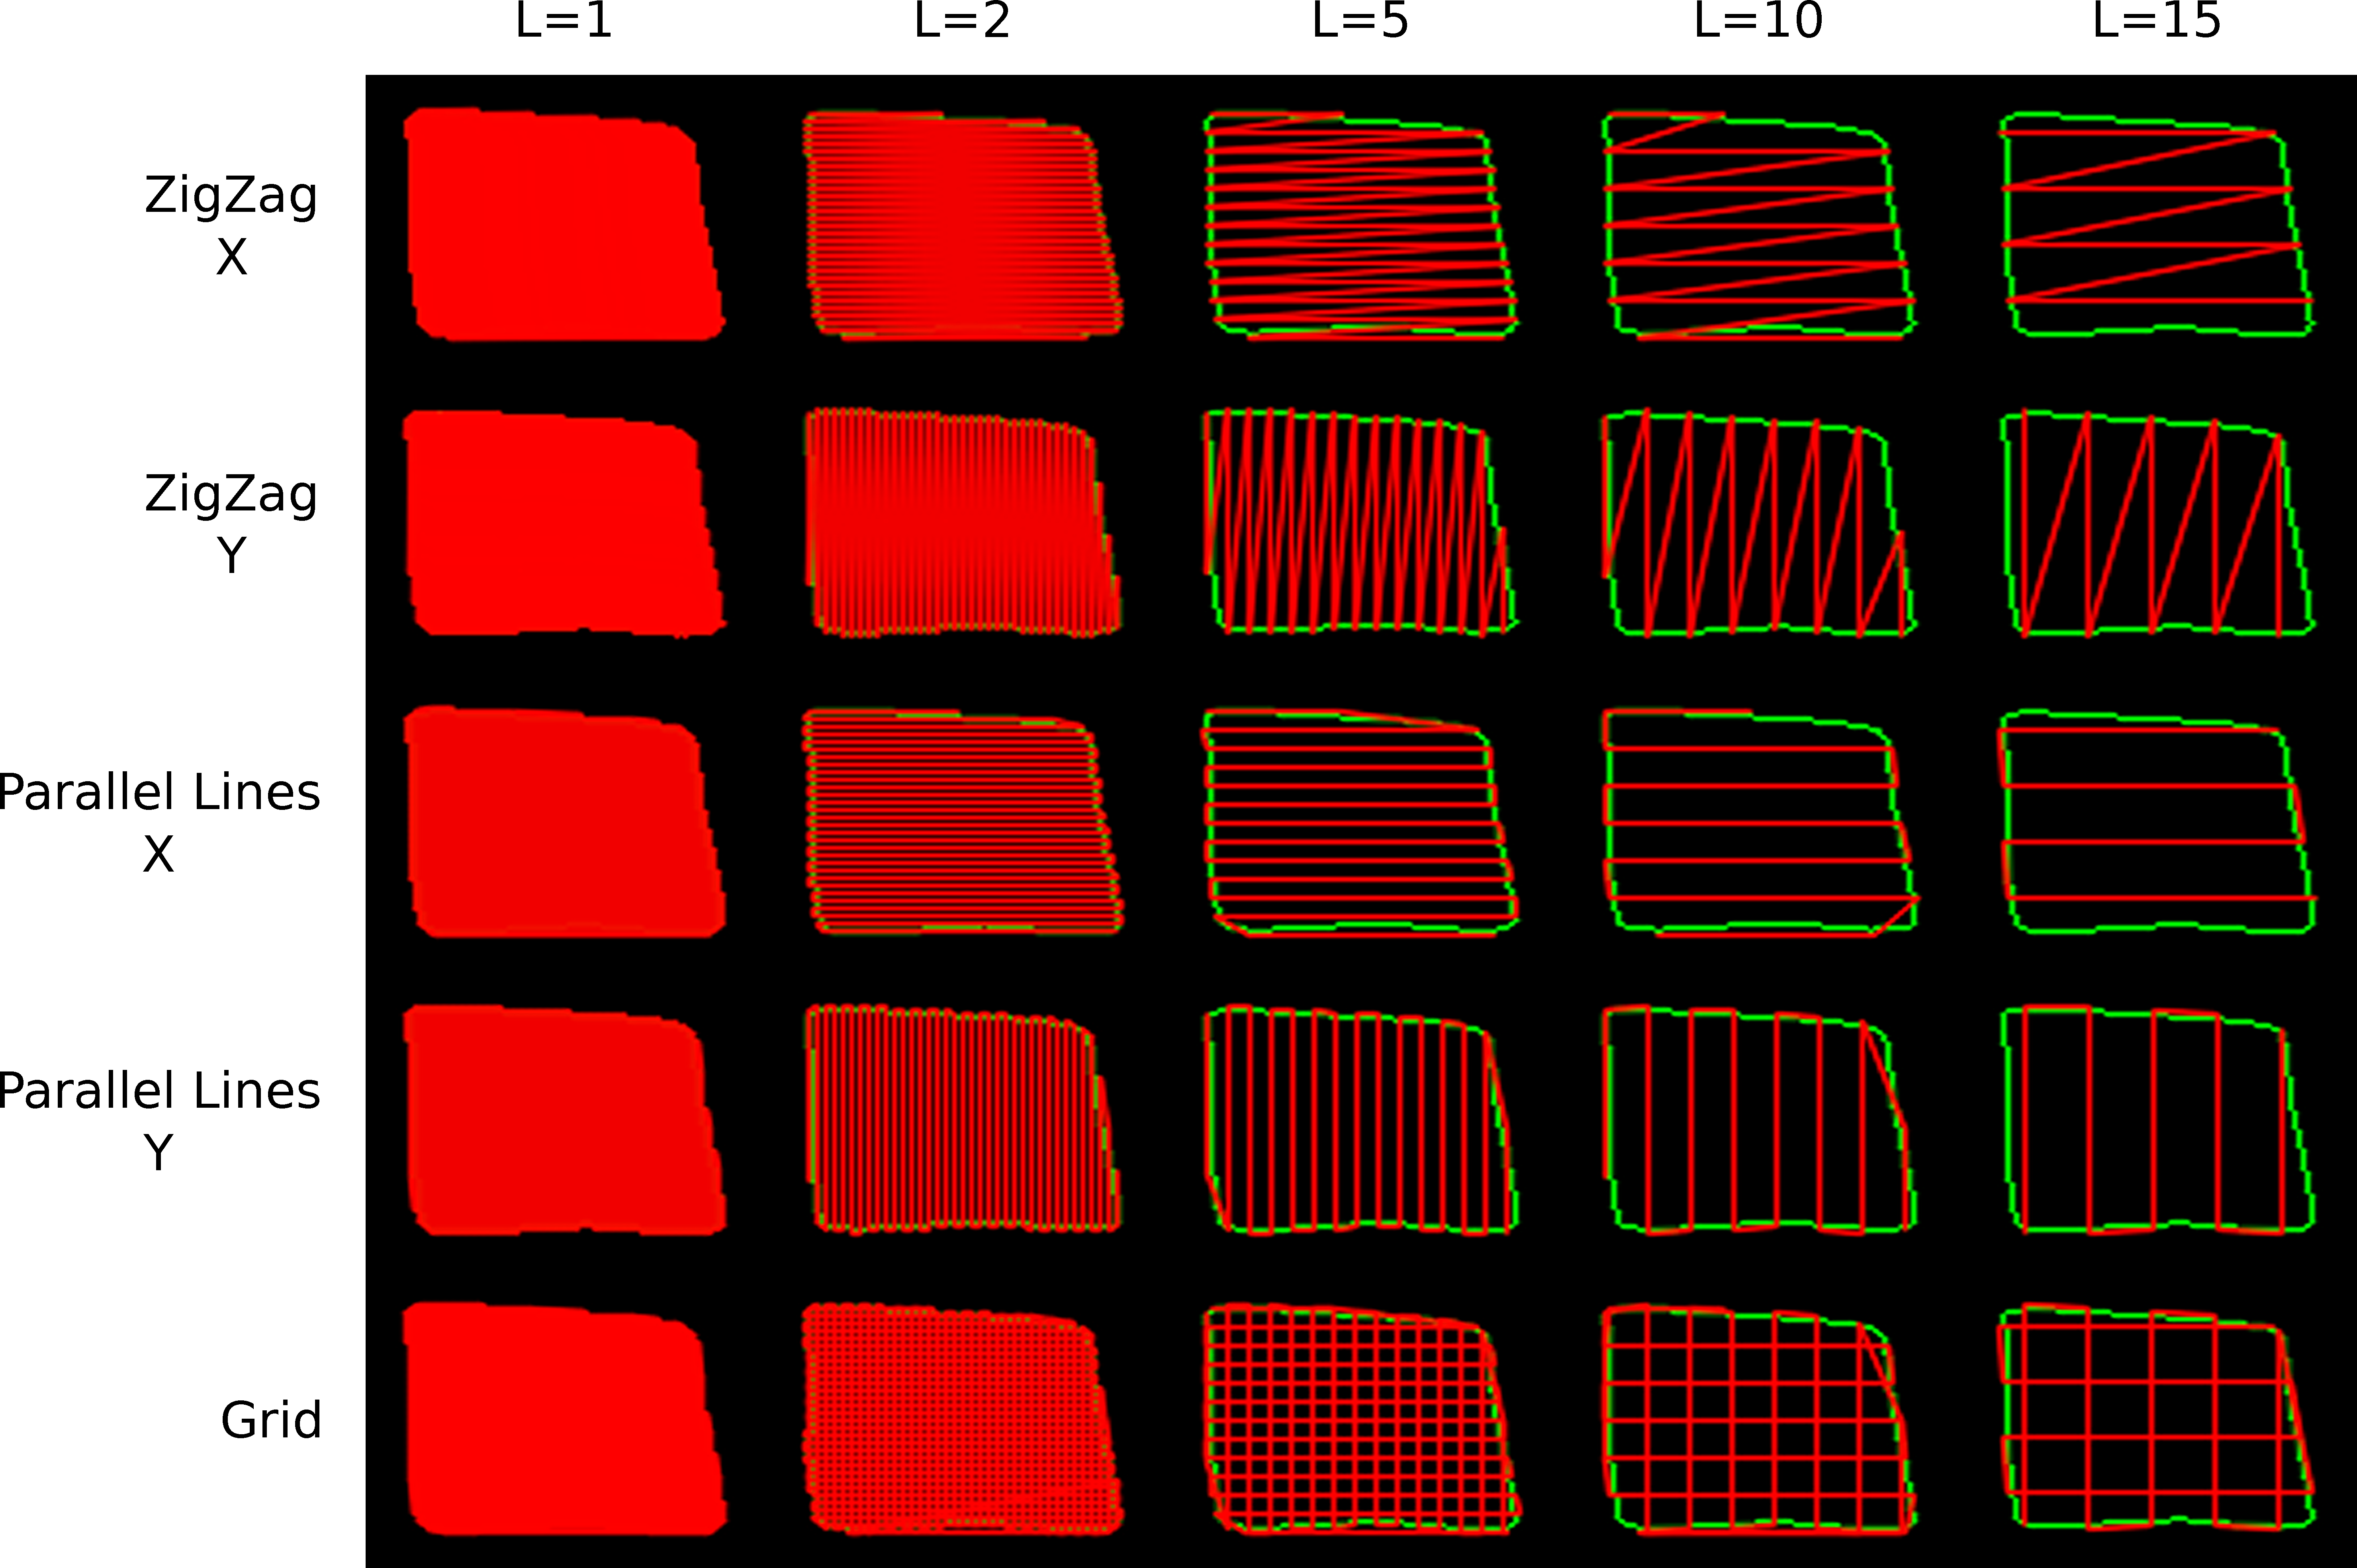
\includegraphics[width=.85\textwidth]{simulation_test_results_appendix_toolpath_wound_1}
	\caption[Path planning for wound model 1.]{Path planning for wound model 1. The green line represents the segmented wound contour. The red line is the planned path. From left to right, the distance between lines, $L$, in pixels, is increasing. Smaller $L$ means more wound filling but also more bioink consumption. From top top bottom, the different paths are displayed. Each line corresponds to a different path planning strategy.}
	\label{fig:simulation_test_results_appendix_toolpath_wound_1}
\end{figure}

\begin{figure}[htbp]
	\centering
	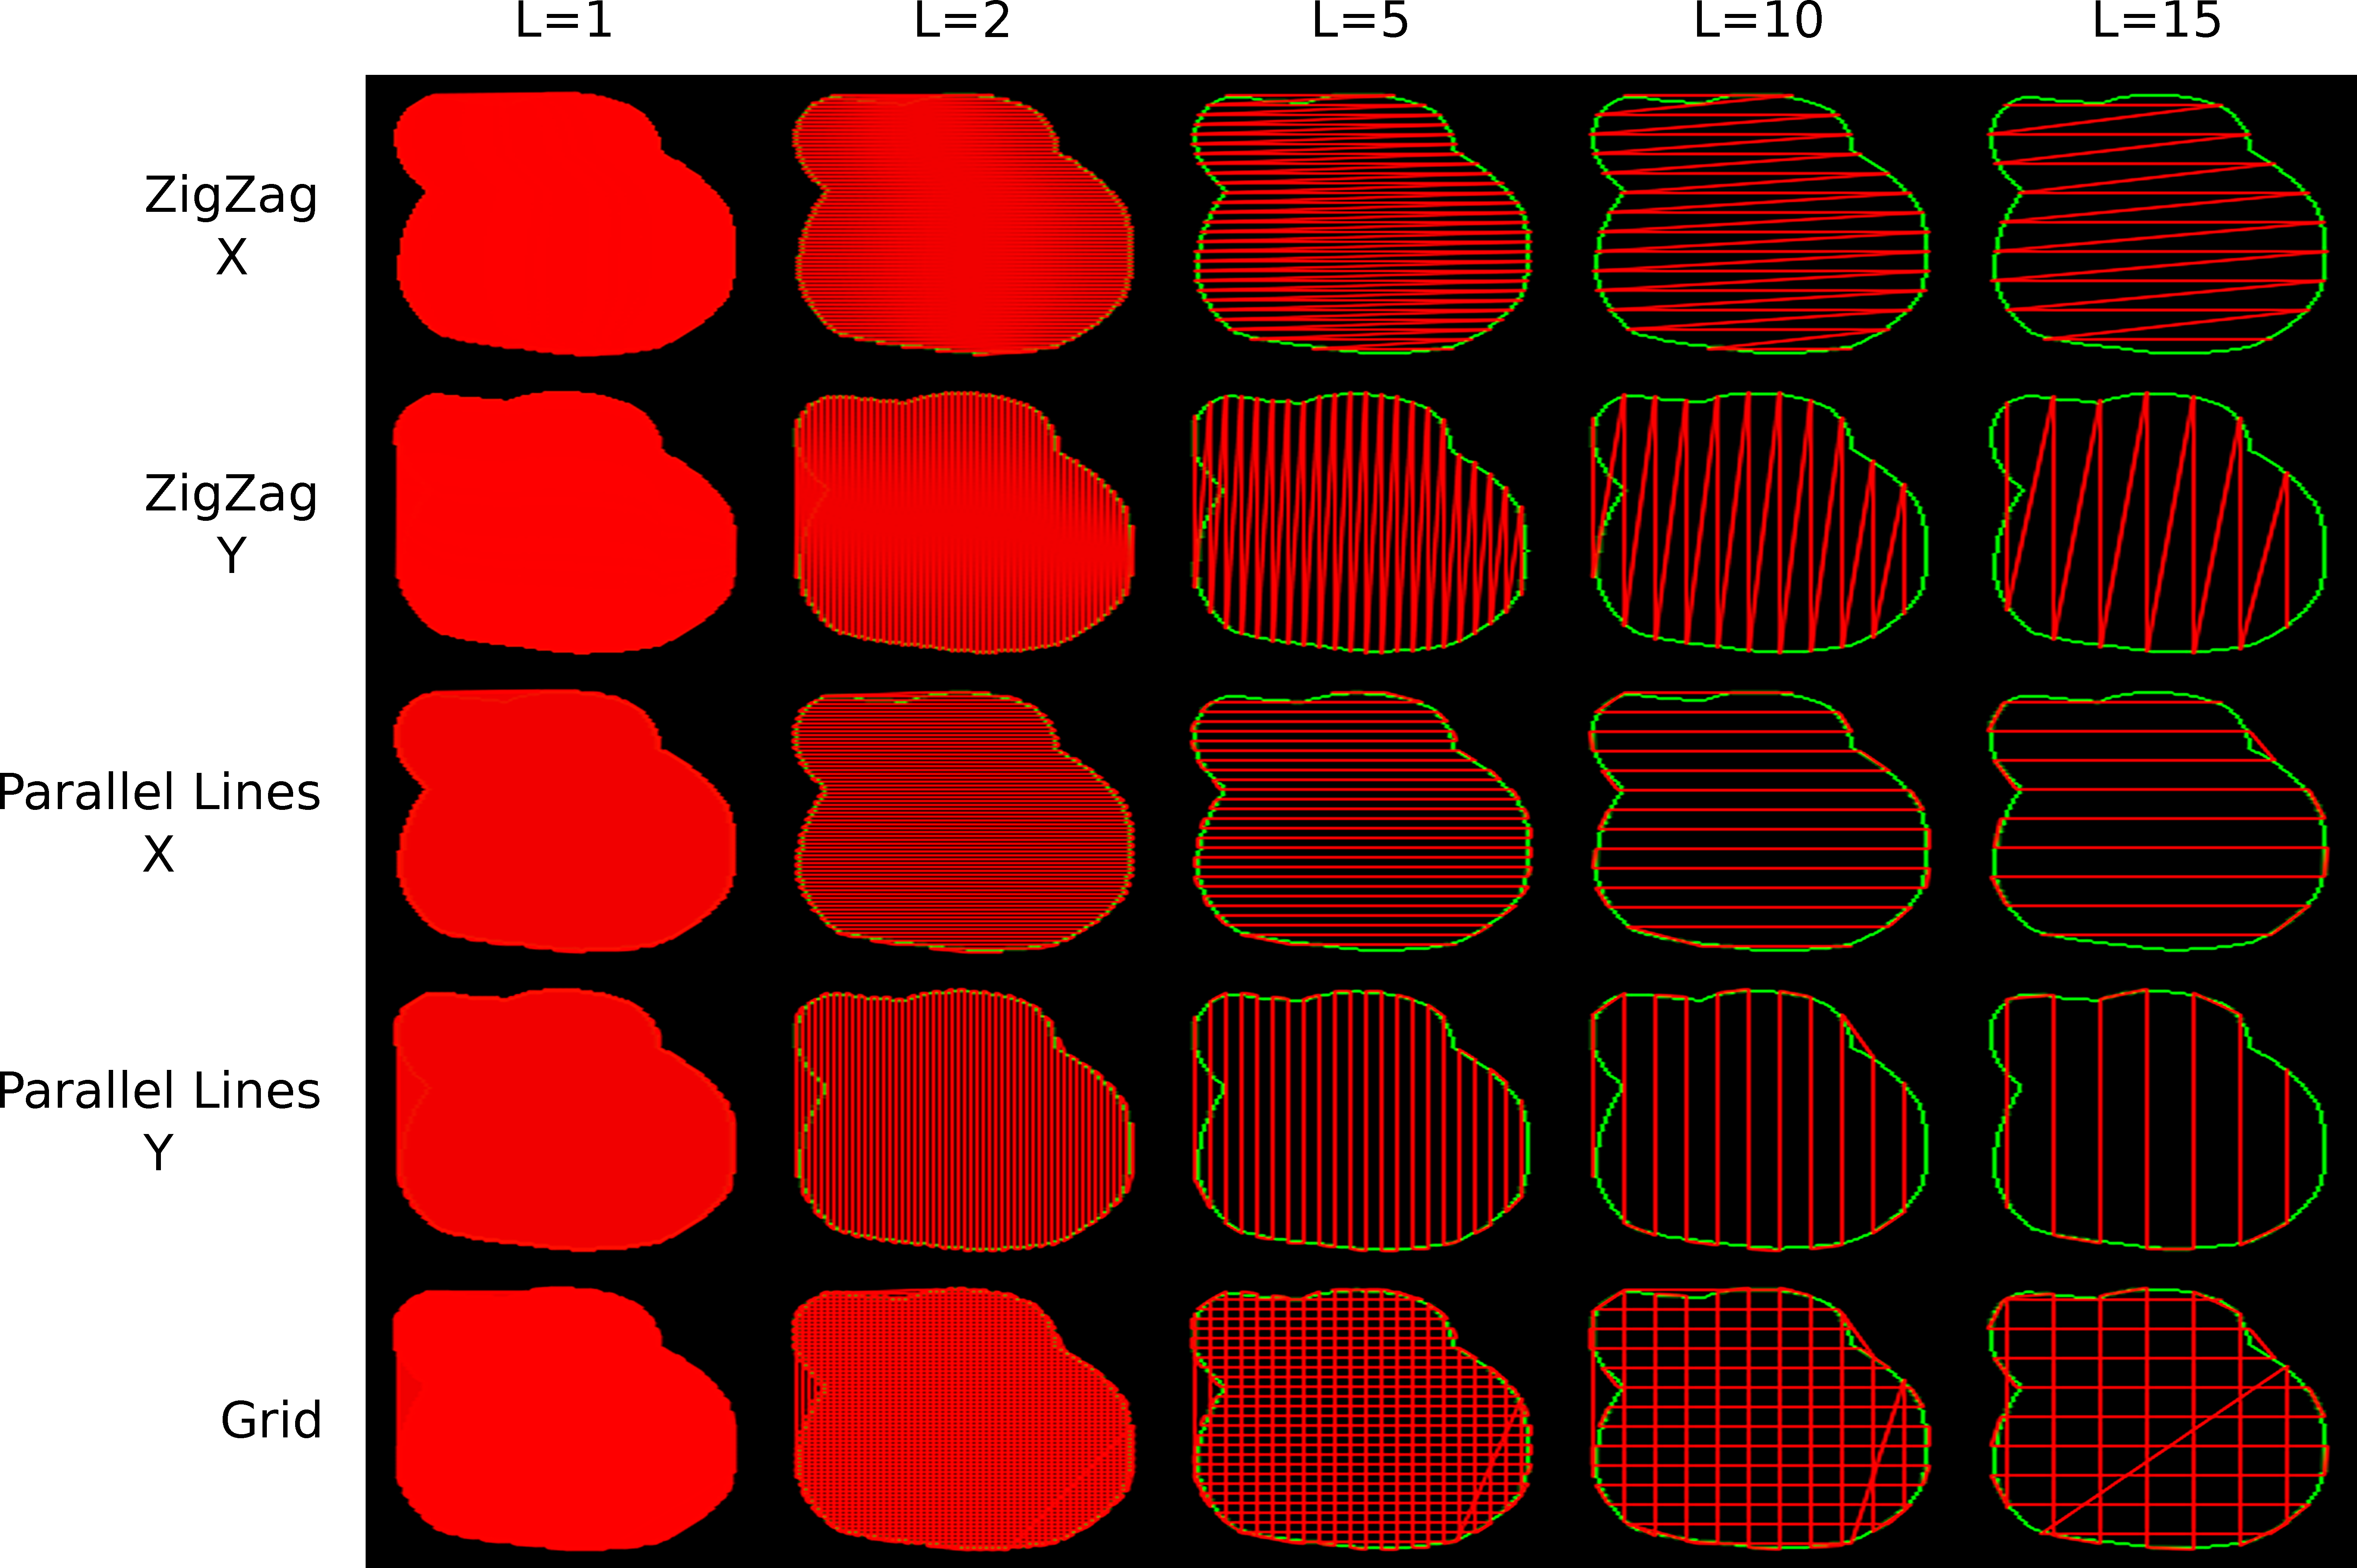
\includegraphics[width=.85\textwidth]{simulation_test_results_appendix_toolpath_wound_2}
	\caption[Path planning for wound model 2.]{Path planning for wound model 2. The green line represents the segmented wound contour. The red line is the planned path. From left to right, the distance between lines, $L$, in pixels, is increasing. Smaller $L$ means more wound filling but also more bioink consumption. From top top bottom, the different paths are displayed. Each line corresponds to a different path planning strategy.}
	\label{fig:simulation_test_results_appendix_toolpath_wound_2}
\end{figure}

\begin{figure}[htbp]
	\centering
	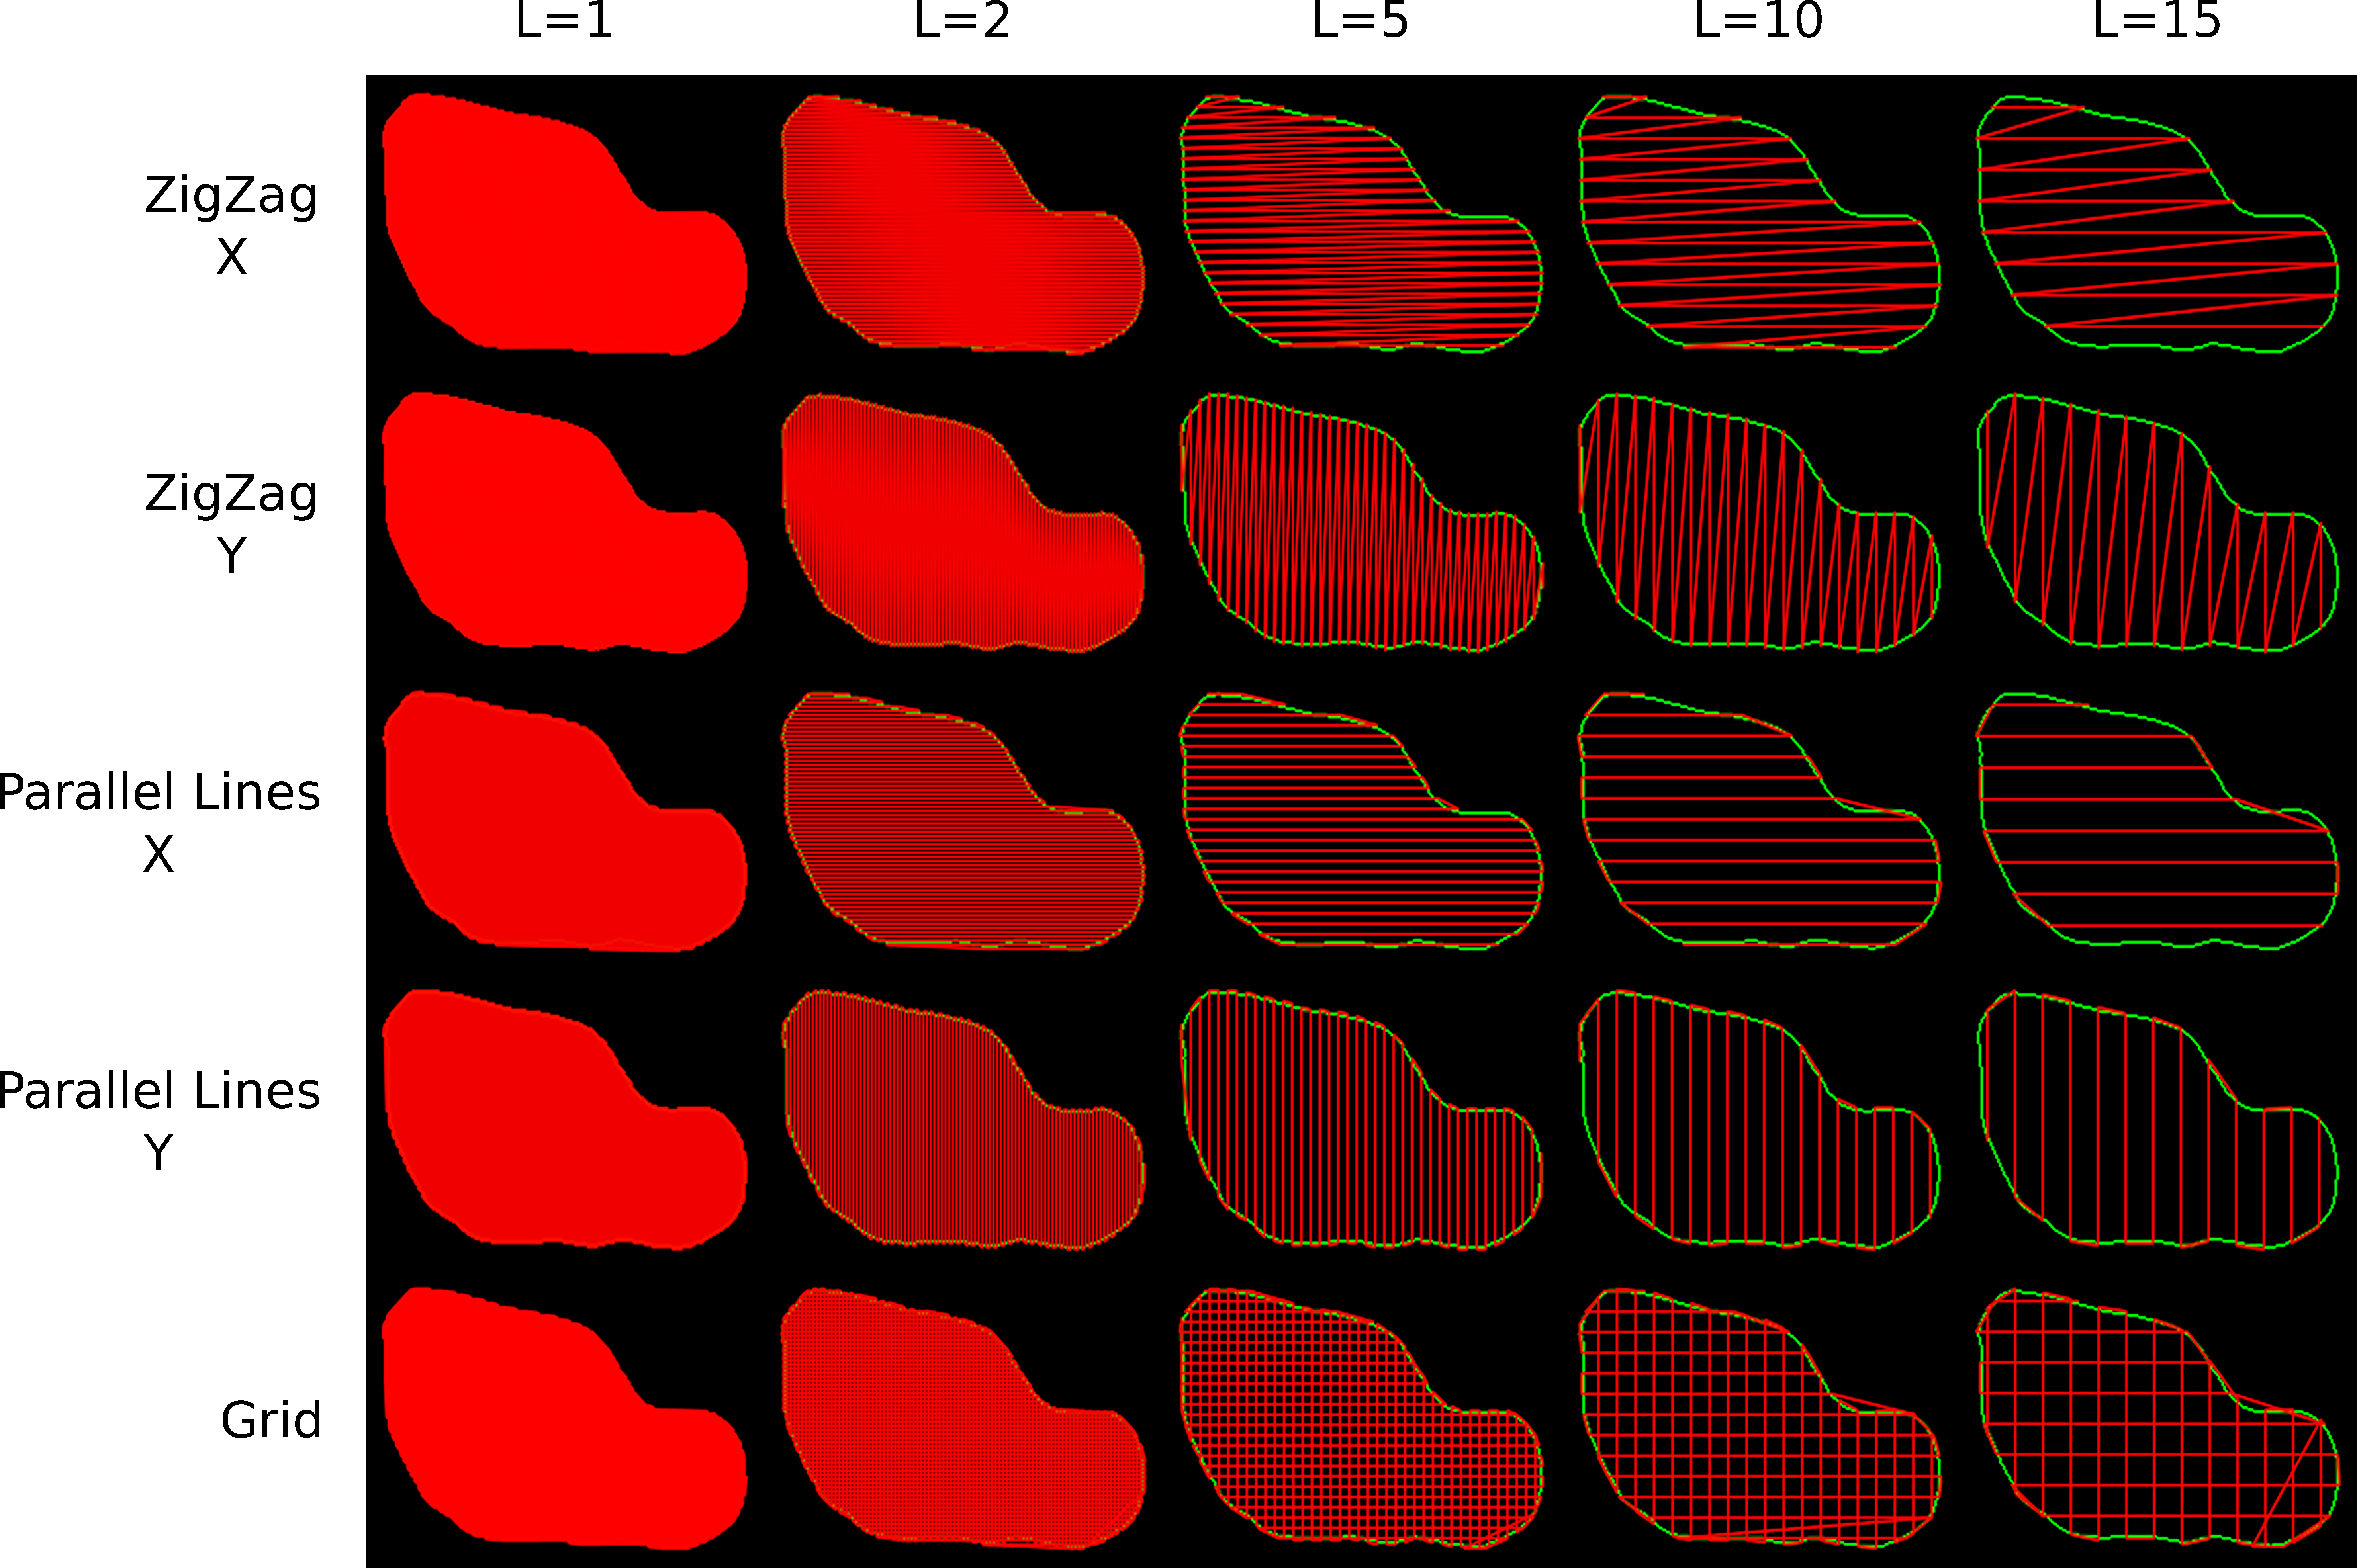
\includegraphics[width=.85\textwidth]{simulation_test_results_appendix_toolpath_wound_3}
	\caption[Path planning for wound model 3.]{Path planning for wound model 3. The green line represents the segmented wound contour. The red line is the planned path. From left to right, the distance between lines, $L$, in pixels, is increasing. Smaller $L$ means more wound filling but also more bioink consumption. From top top bottom, the different paths are displayed. Each line corresponds to a different path planning strategy.}
	\label{fig:simulation_test_results_appendix_toolpath_wound_3}
\end{figure}

\begin{figure}[htbp]
	\centering
	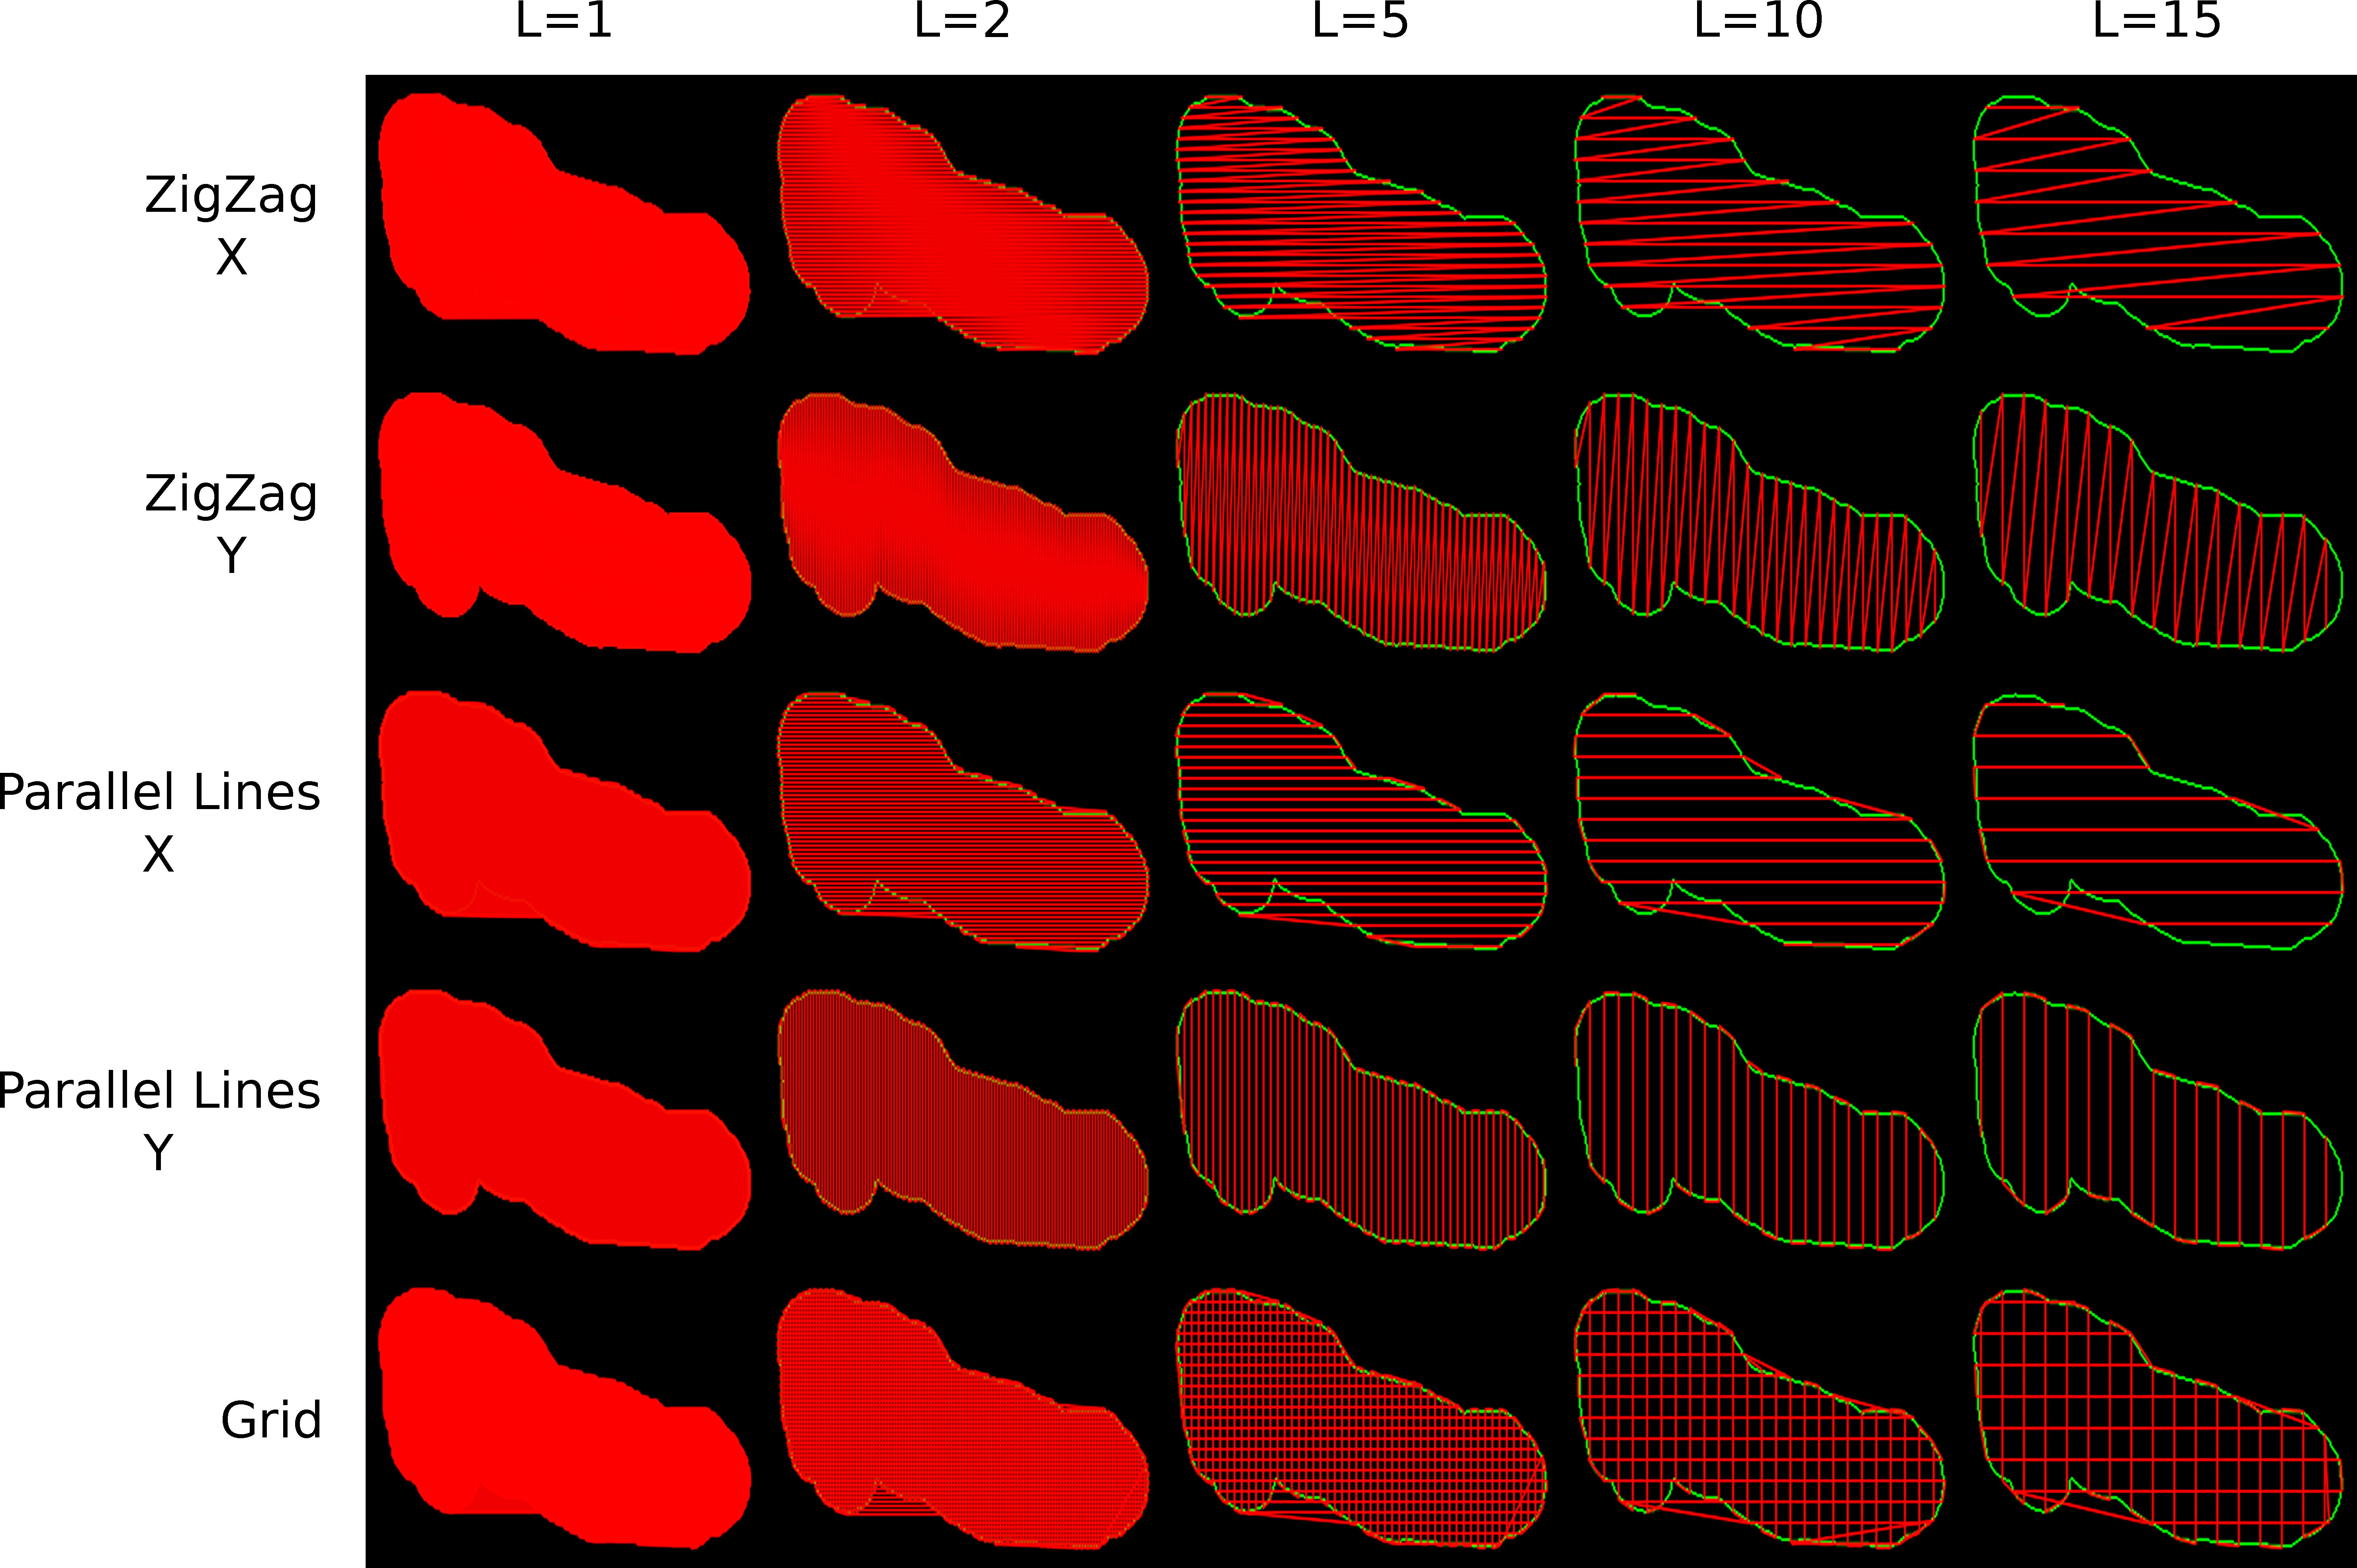
\includegraphics[width=.85\textwidth]{simulation_test_results_appendix_toolpath_wound_4}
	\caption[Path planning for wound model 4.]{Path planning for wound model 4. The green line represents the segmented wound contour. The red line is the planned path. From left to right, the distance between lines, $L$, in pixels, is increasing. Smaller $L$ means more wound filling but also more bioink consumption. From top top bottom, the different paths are displayed. Each line corresponds to a different path planning strategy.}
	\label{fig:simulation_test_results_appendix_toolpath_wound_4}
\end{figure}

\begin{figure}[htbp]
	\centering
	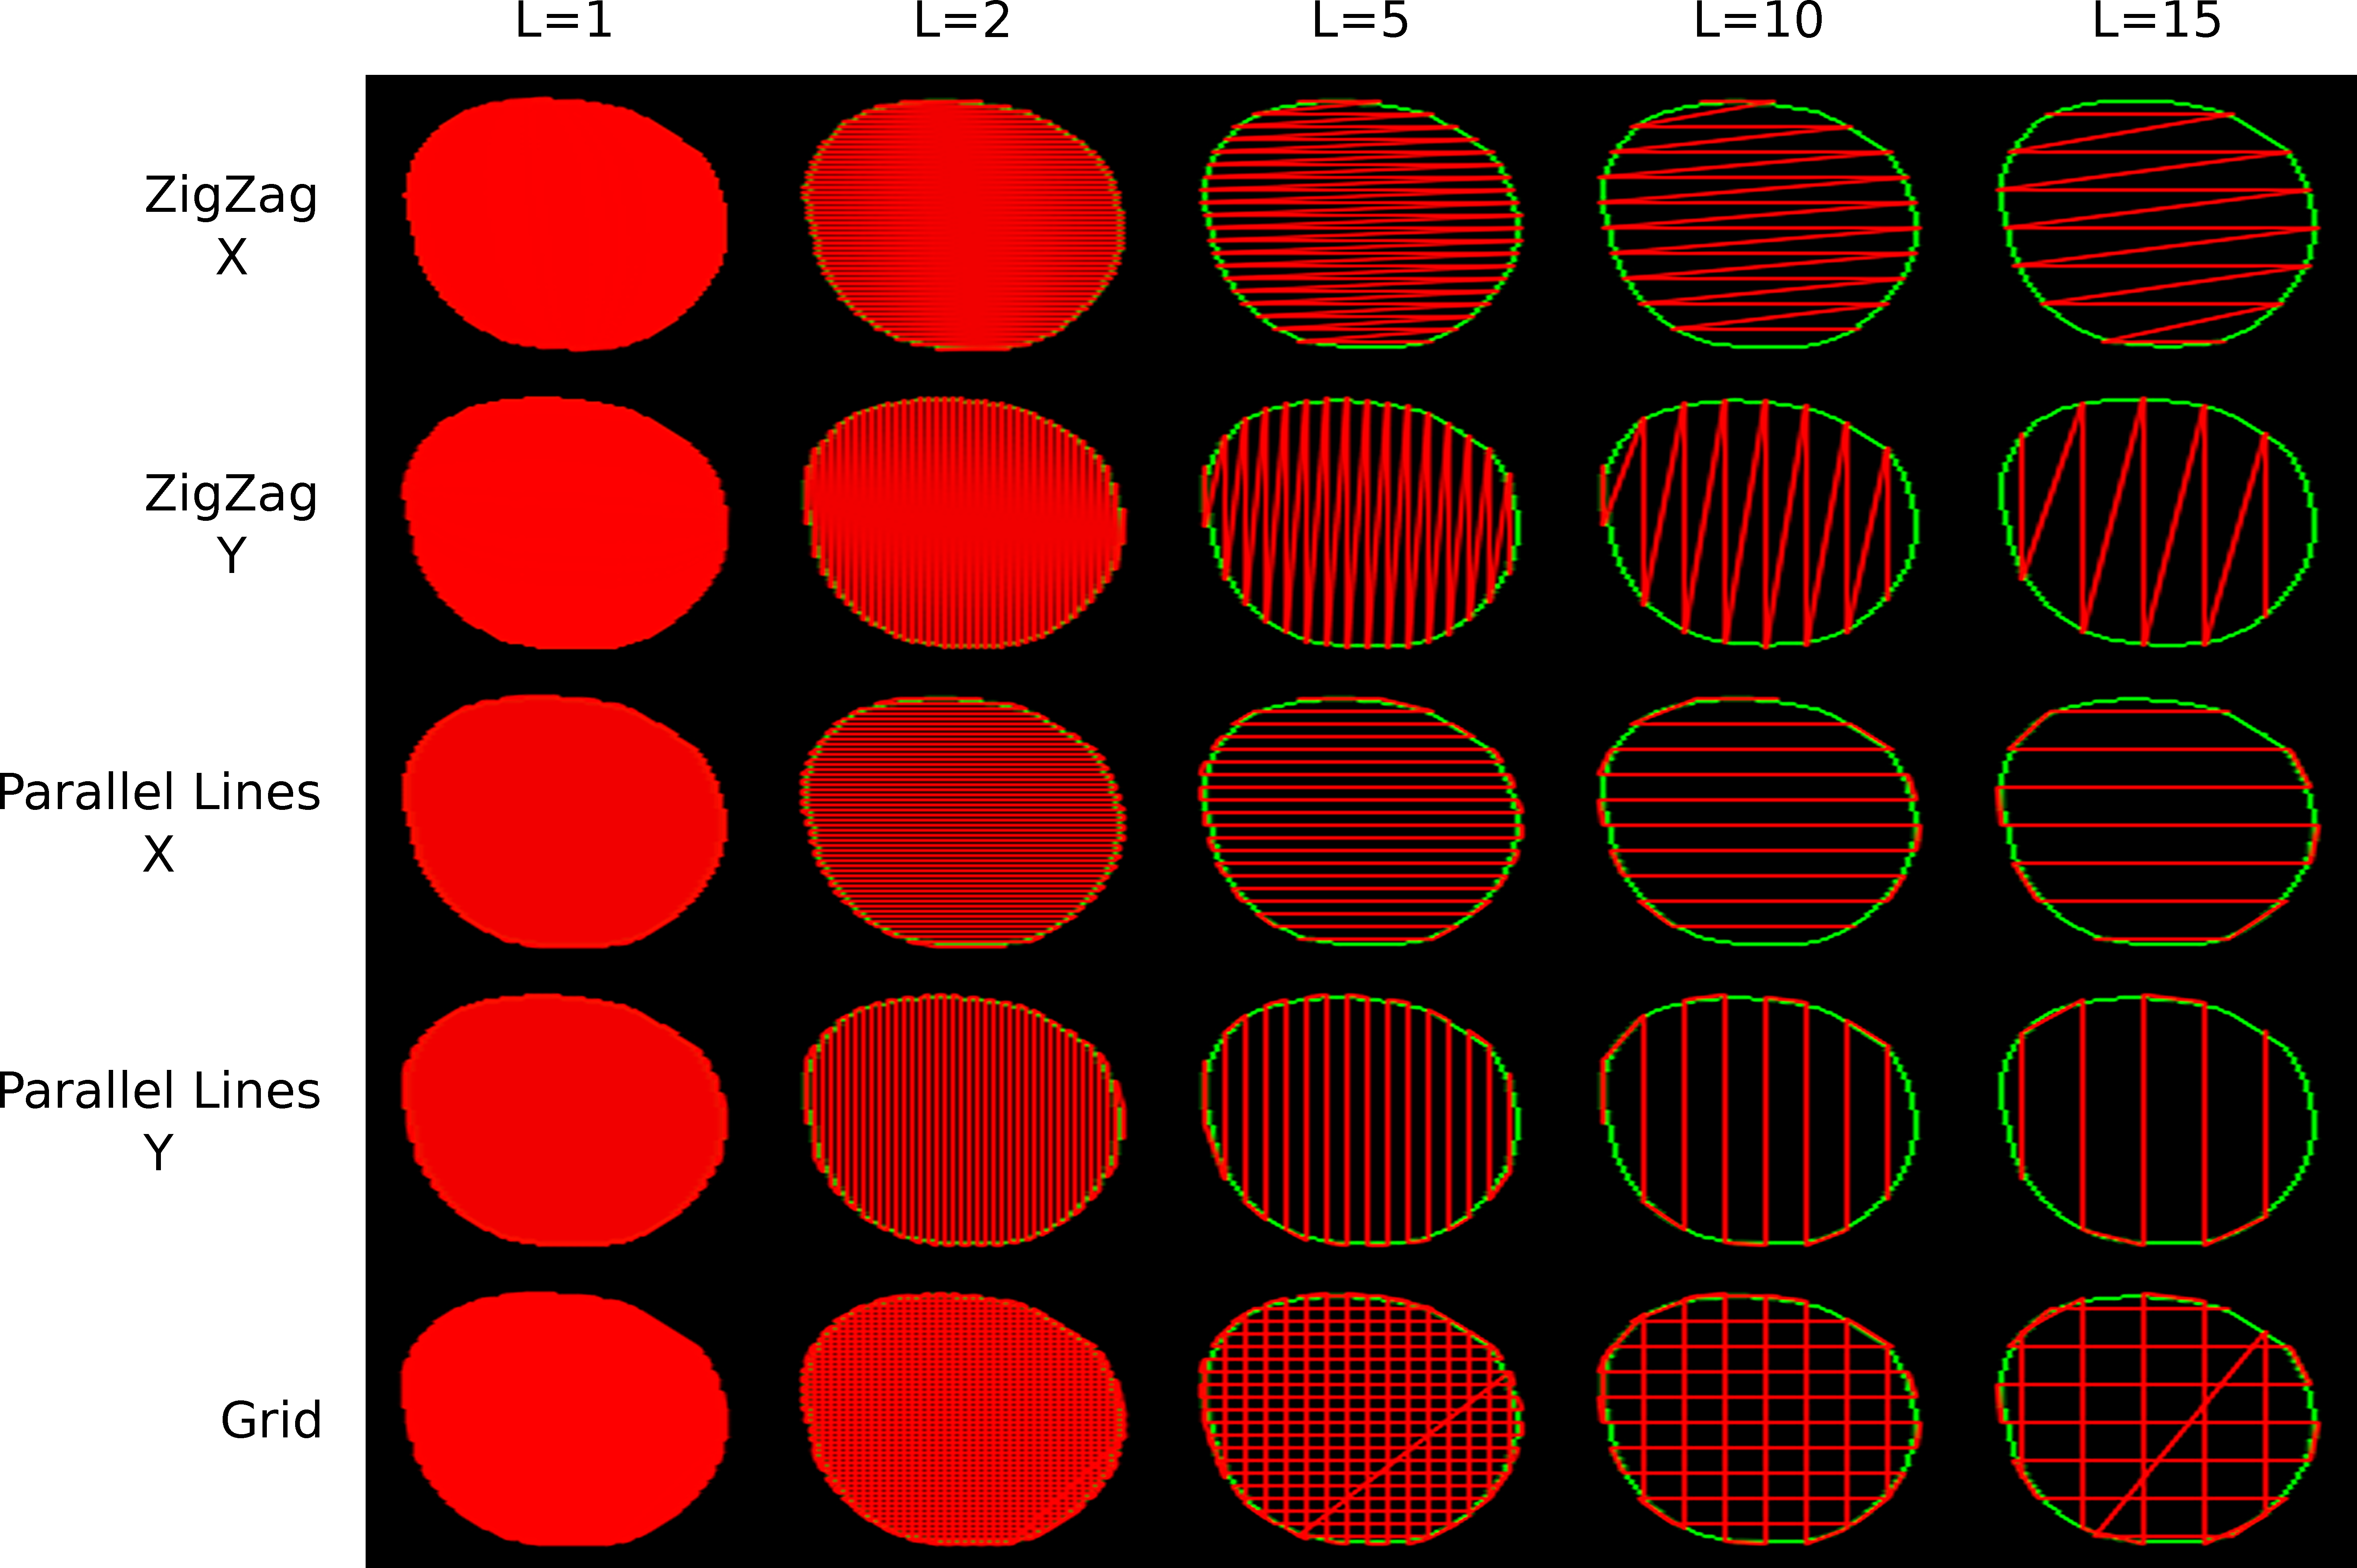
\includegraphics[width=.85\textwidth]{simulation_test_results_appendix_toolpath_wound_5}
	\caption[Path planning for wound model 5.]{Path planning for wound model 5. The green line represents the segmented wound contour. The red line is the planned path. From left to right, the distance between lines, $L$, in pixels, is increasing. Smaller $L$ means more wound filling but also more bioink consumption. From top top bottom, the different paths are displayed. Each line corresponds to a different path planning strategy.}
	\label{fig:simulation_test_results_appendix_toolpath_wound_5}
\end{figure}

% section simulation_test_results_appendix_path_planning

\clearpage

\section{3D Bioprinting Directly on Wound}
\label{sec:simulation_test_results_appendix_bioprinting_directly_wound}

This section presents the results of the robot tracking errors, and printing trajectory.

\begin{figure}[htbp]
	\centering
	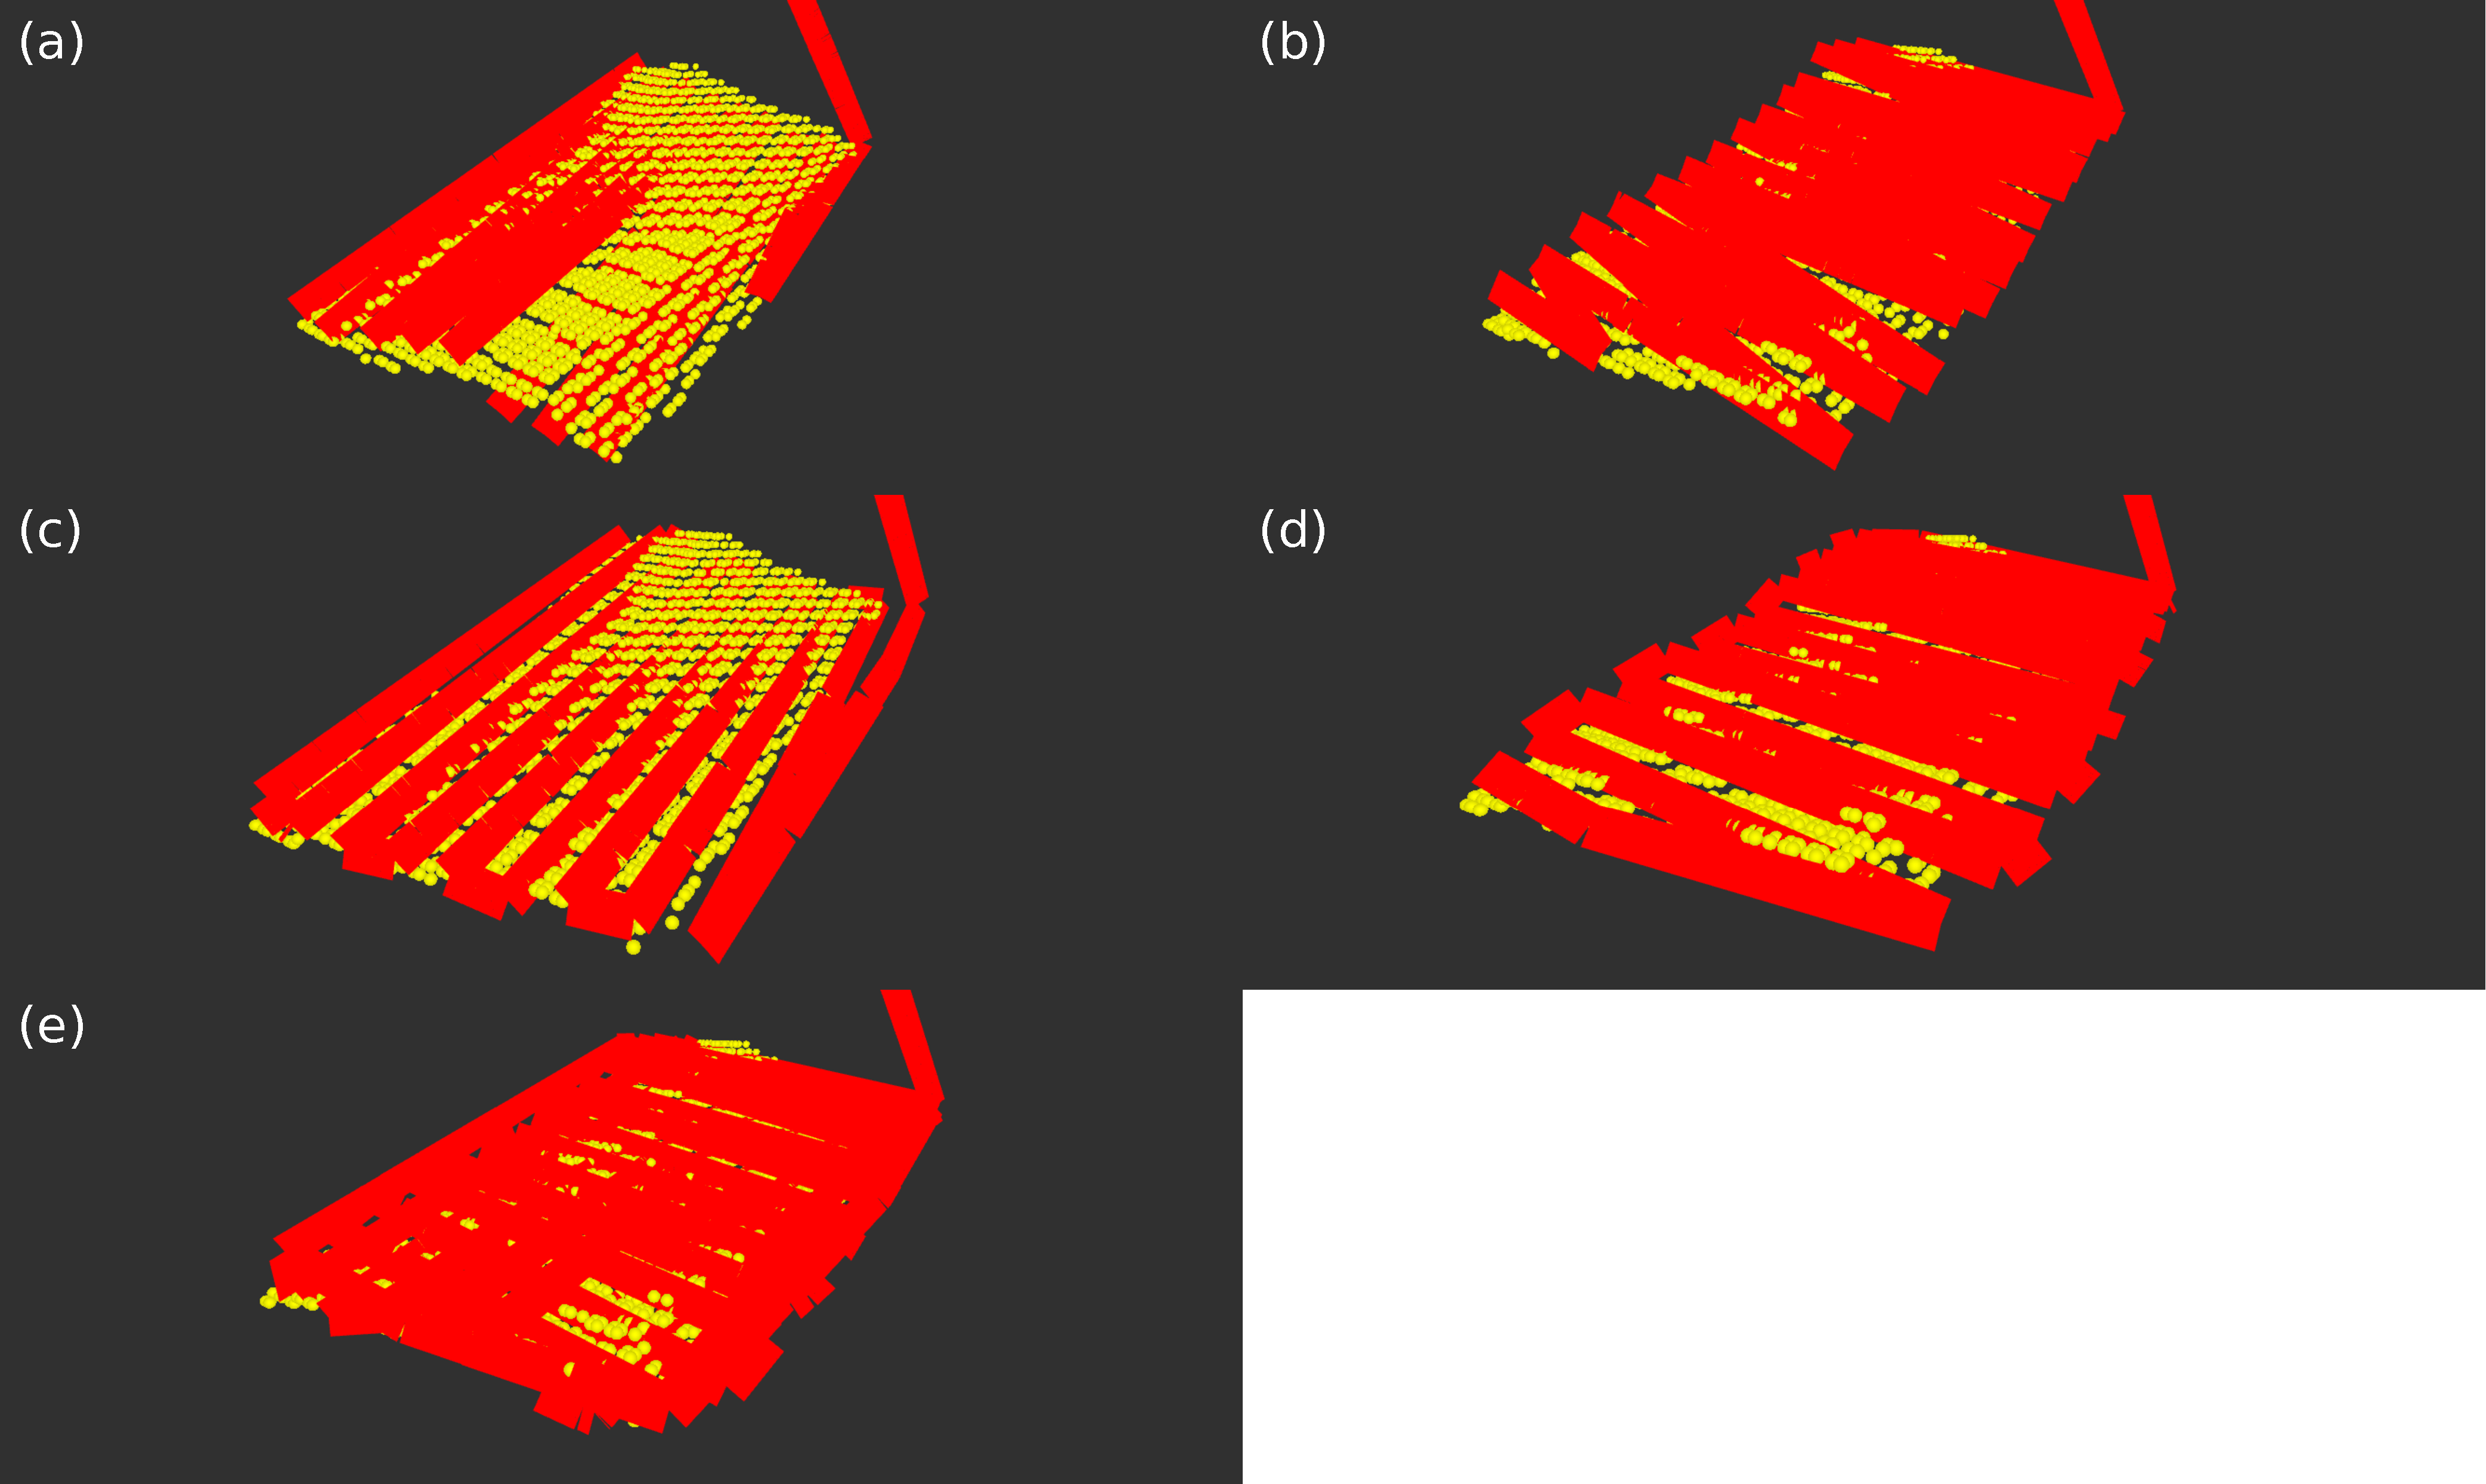
\includegraphics[width=\textwidth]{simulation_test_results_appendix_trajectory_wound_1}
	\caption[Wound 1 printing trajectory.]{Wound 1 printing trajectory. (a) ZigZag X, (b) ZigZag Y, (c) Parallel Lines X, (d) Parallel Lines Y, and (e) Grid path. All paths used $L = 5$.}
    \label{fig:simulation_test_results_appendix_trajectory_wound_1}
\end{figure}

\begin{figure}[htbp]
	\centering
	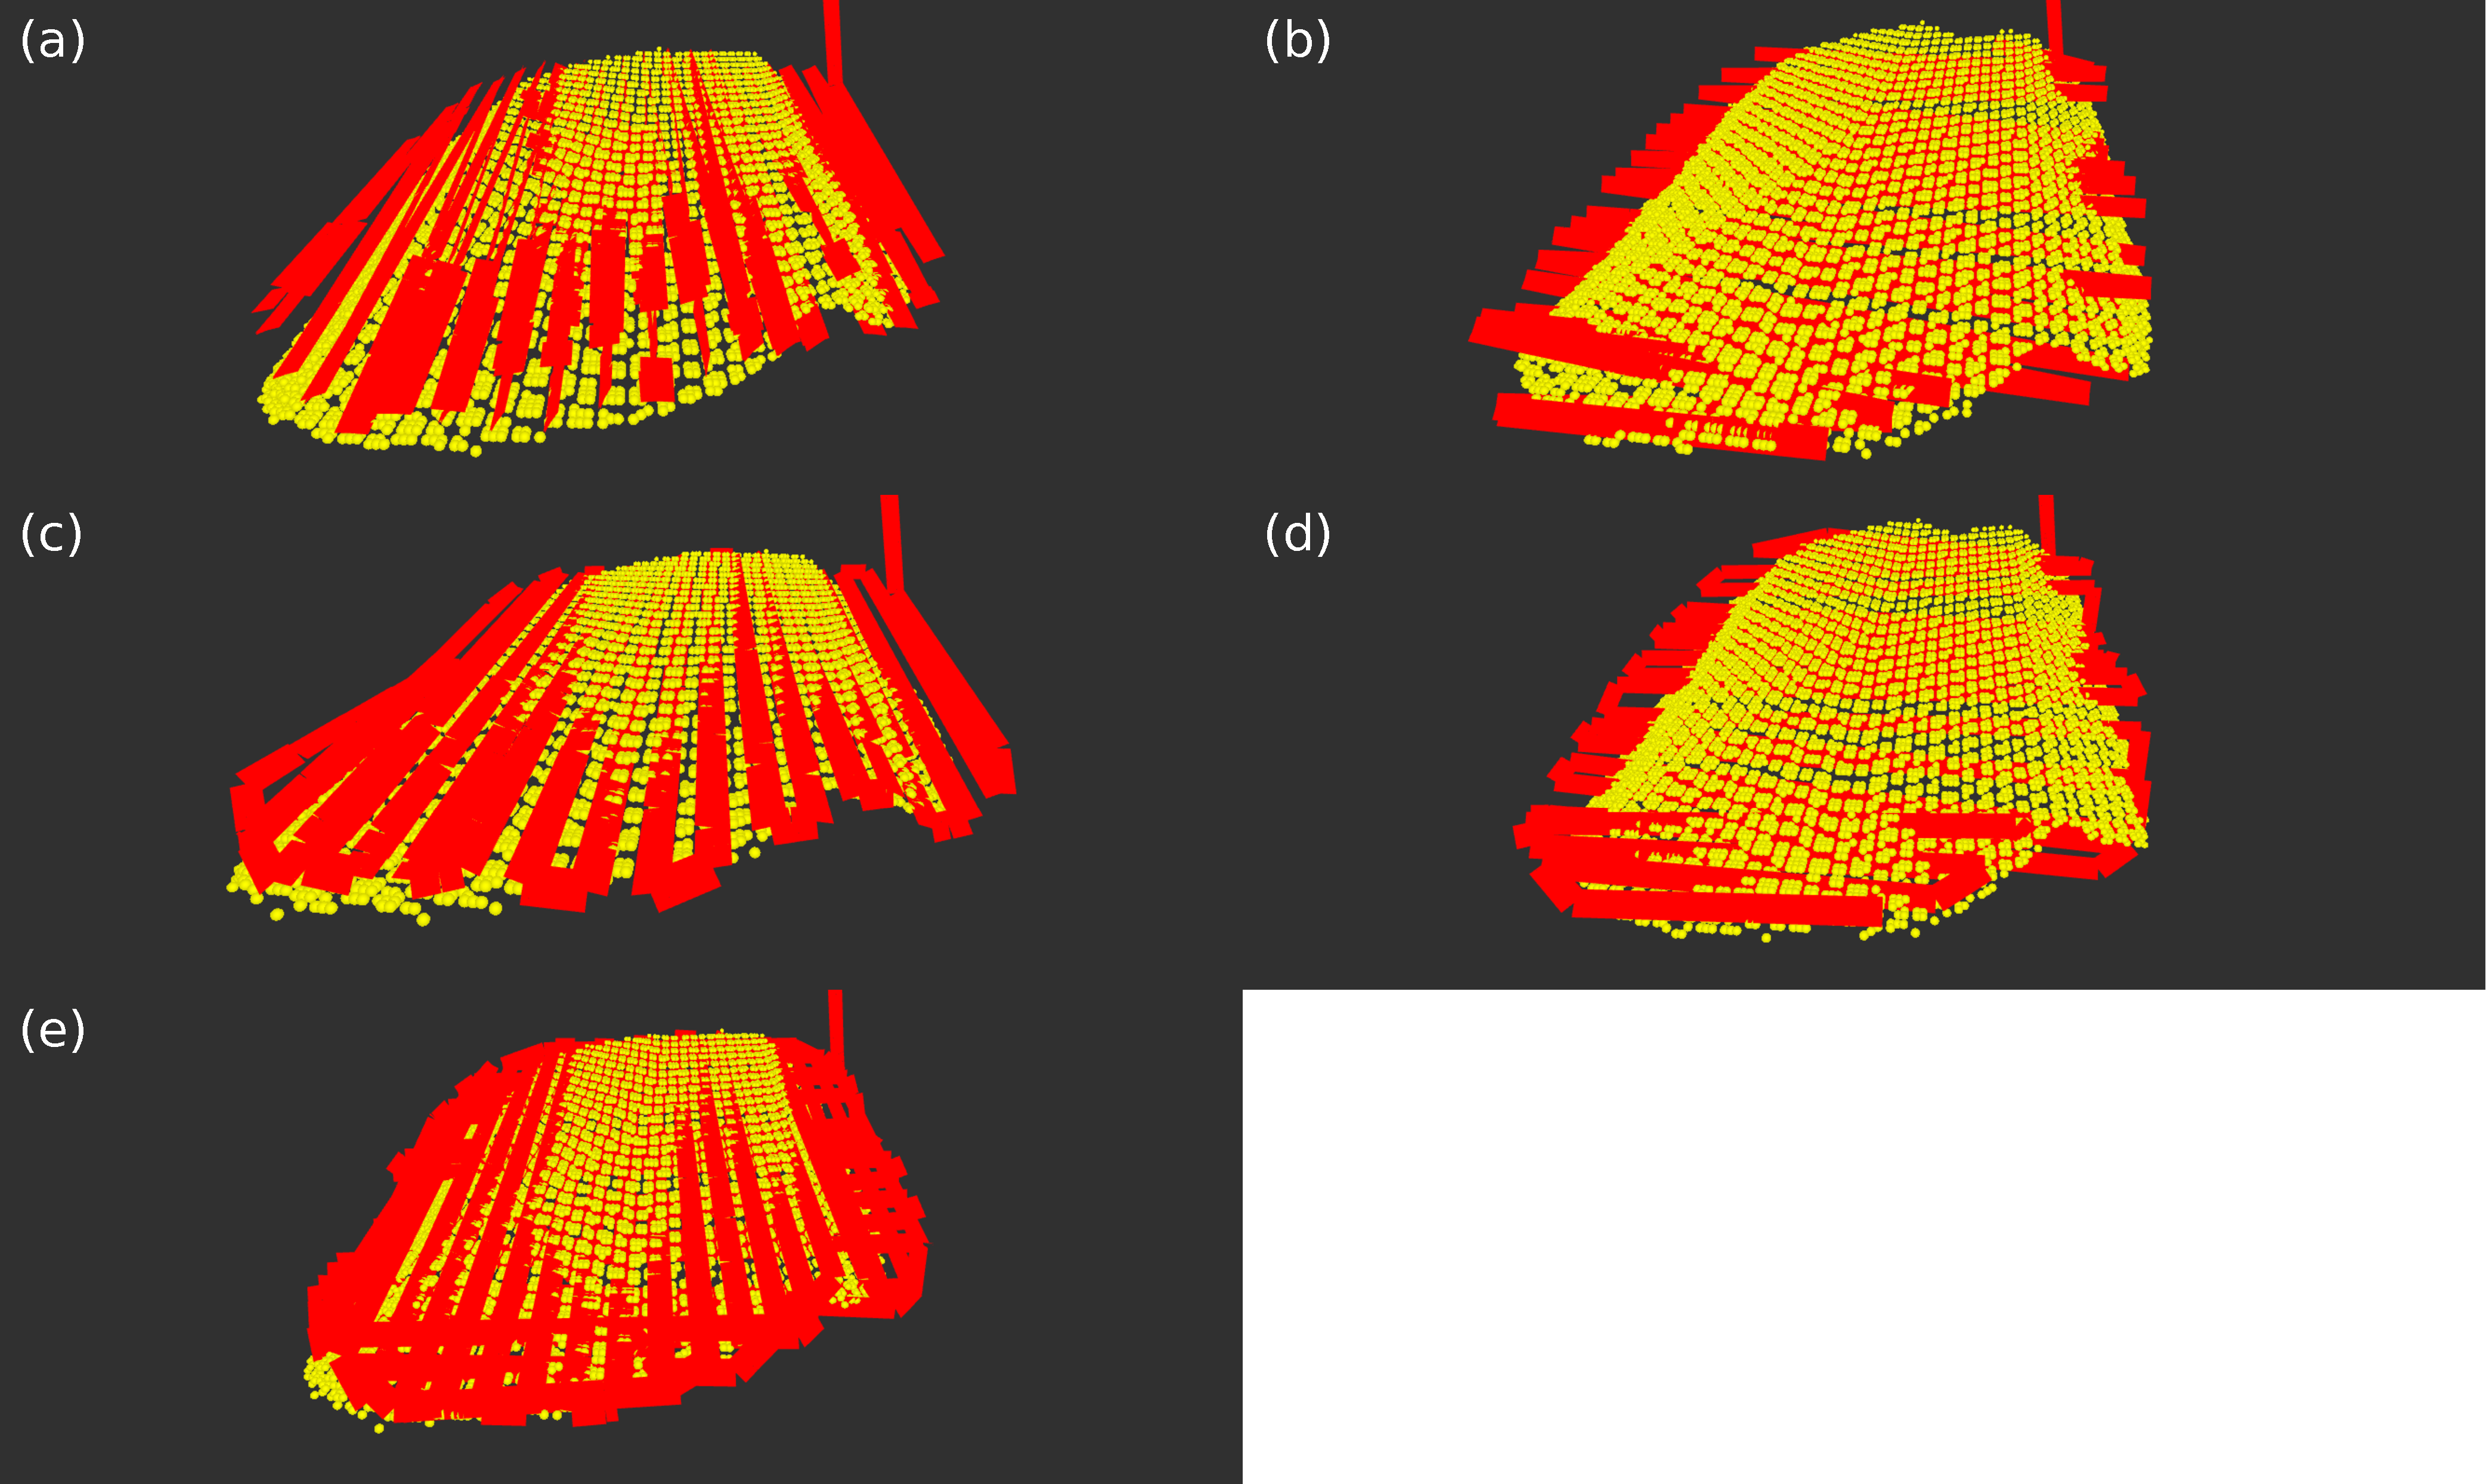
\includegraphics[width=\textwidth]{simulation_test_results_appendix_trajectory_wound_2}
	\caption[Wound 2 printing trajectory.]{Wound 2 printing trajectory. (a) ZigZag X, (b) ZigZag Y, (c) Parallel Lines X, (d) Parallel Lines Y, and (e) Grid path. All paths used $L = 5$.}
    \label{fig:simulation_test_results_appendix_trajectory_wound_2}
\end{figure}

\begin{figure}[htbp]
	\centering
	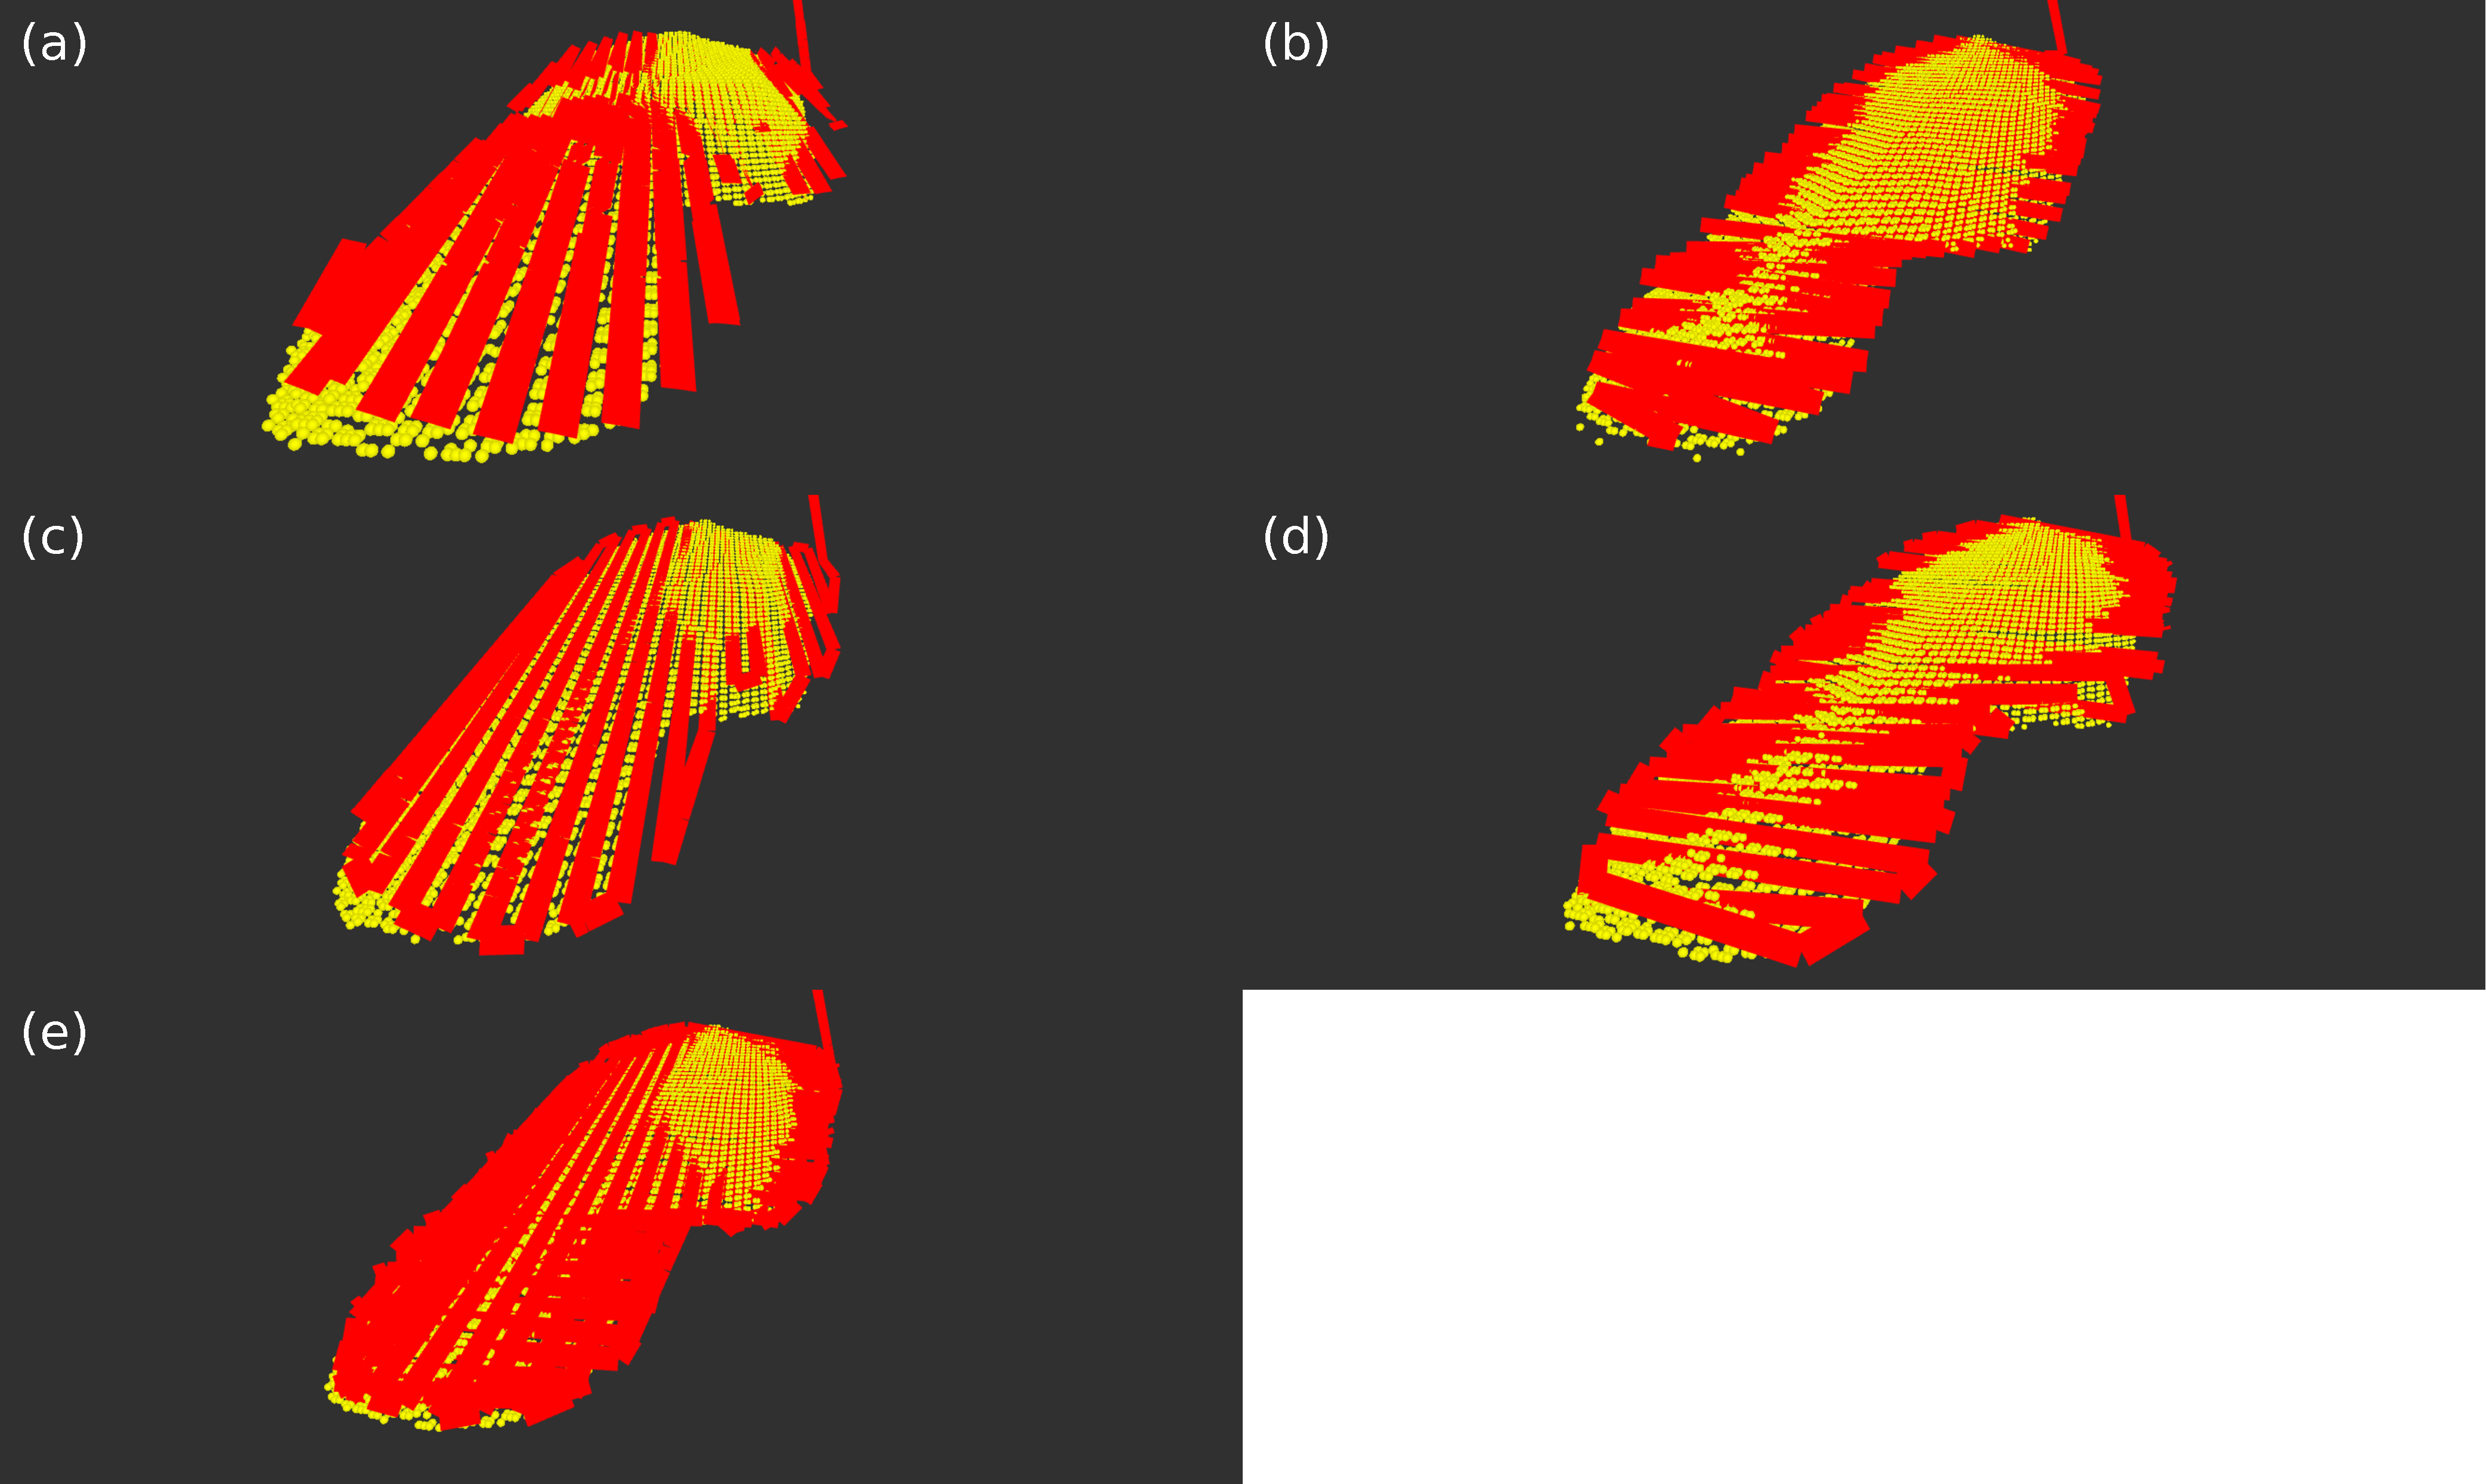
\includegraphics[width=\textwidth]{simulation_test_results_appendix_trajectory_wound_3}
	\caption[Wound 3 printing trajectory.]{Wound 3 printing trajectory. (a) ZigZag X, (b) ZigZag Y, (c) Parallel Lines X, (d) Parallel Lines Y, and (e) Grid path. All paths used $L = 5$.}
    \label{fig:simulation_test_results_appendix_trajectory_wound_3}
\end{figure}

\begin{figure}[htbp]
	\centering
	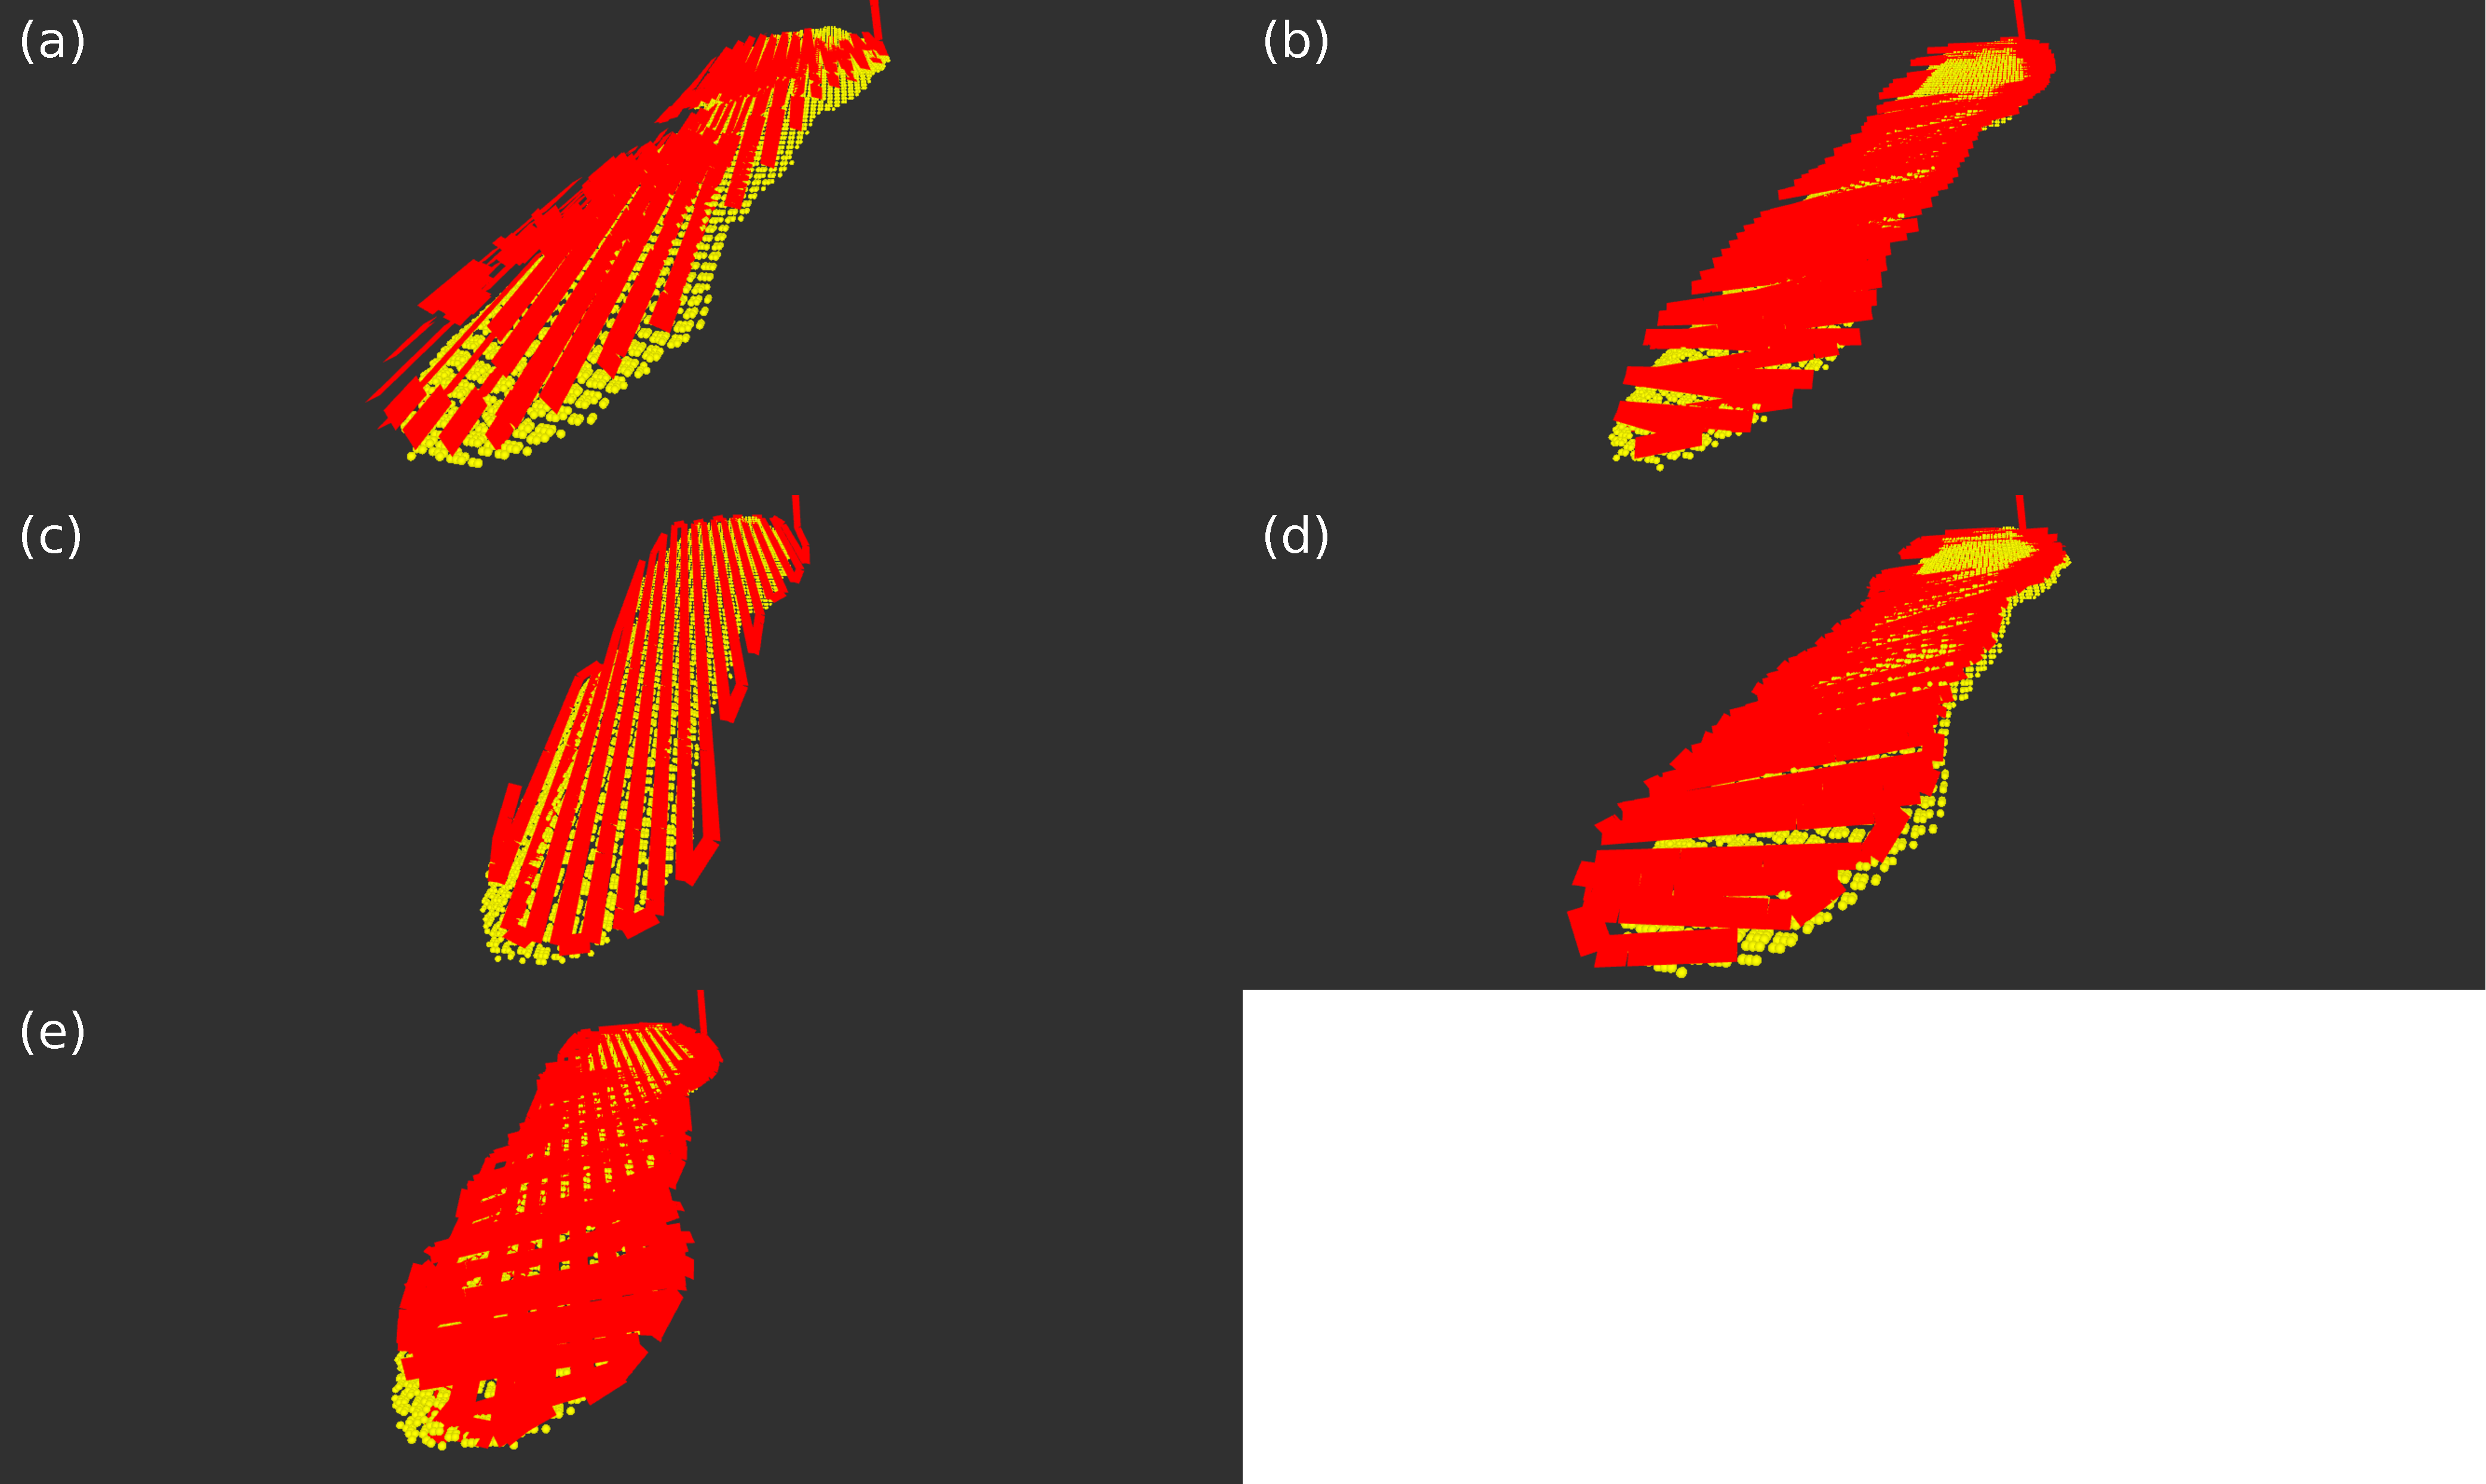
\includegraphics[width=\textwidth]{simulation_test_results_appendix_trajectory_wound_4}
	\caption[Wound 4 printing trajectory.]{Wound 4 printing trajectory. (a) ZigZag X, (b) ZigZag Y, (c) Parallel Lines X, (d) Parallel Lines Y, and (e) Grid path. All paths used $L = 5$.}
    \label{fig:simulation_test_results_appendix_trajectory_wound_4}
\end{figure}

\begin{figure}[htbp]
	\centering
	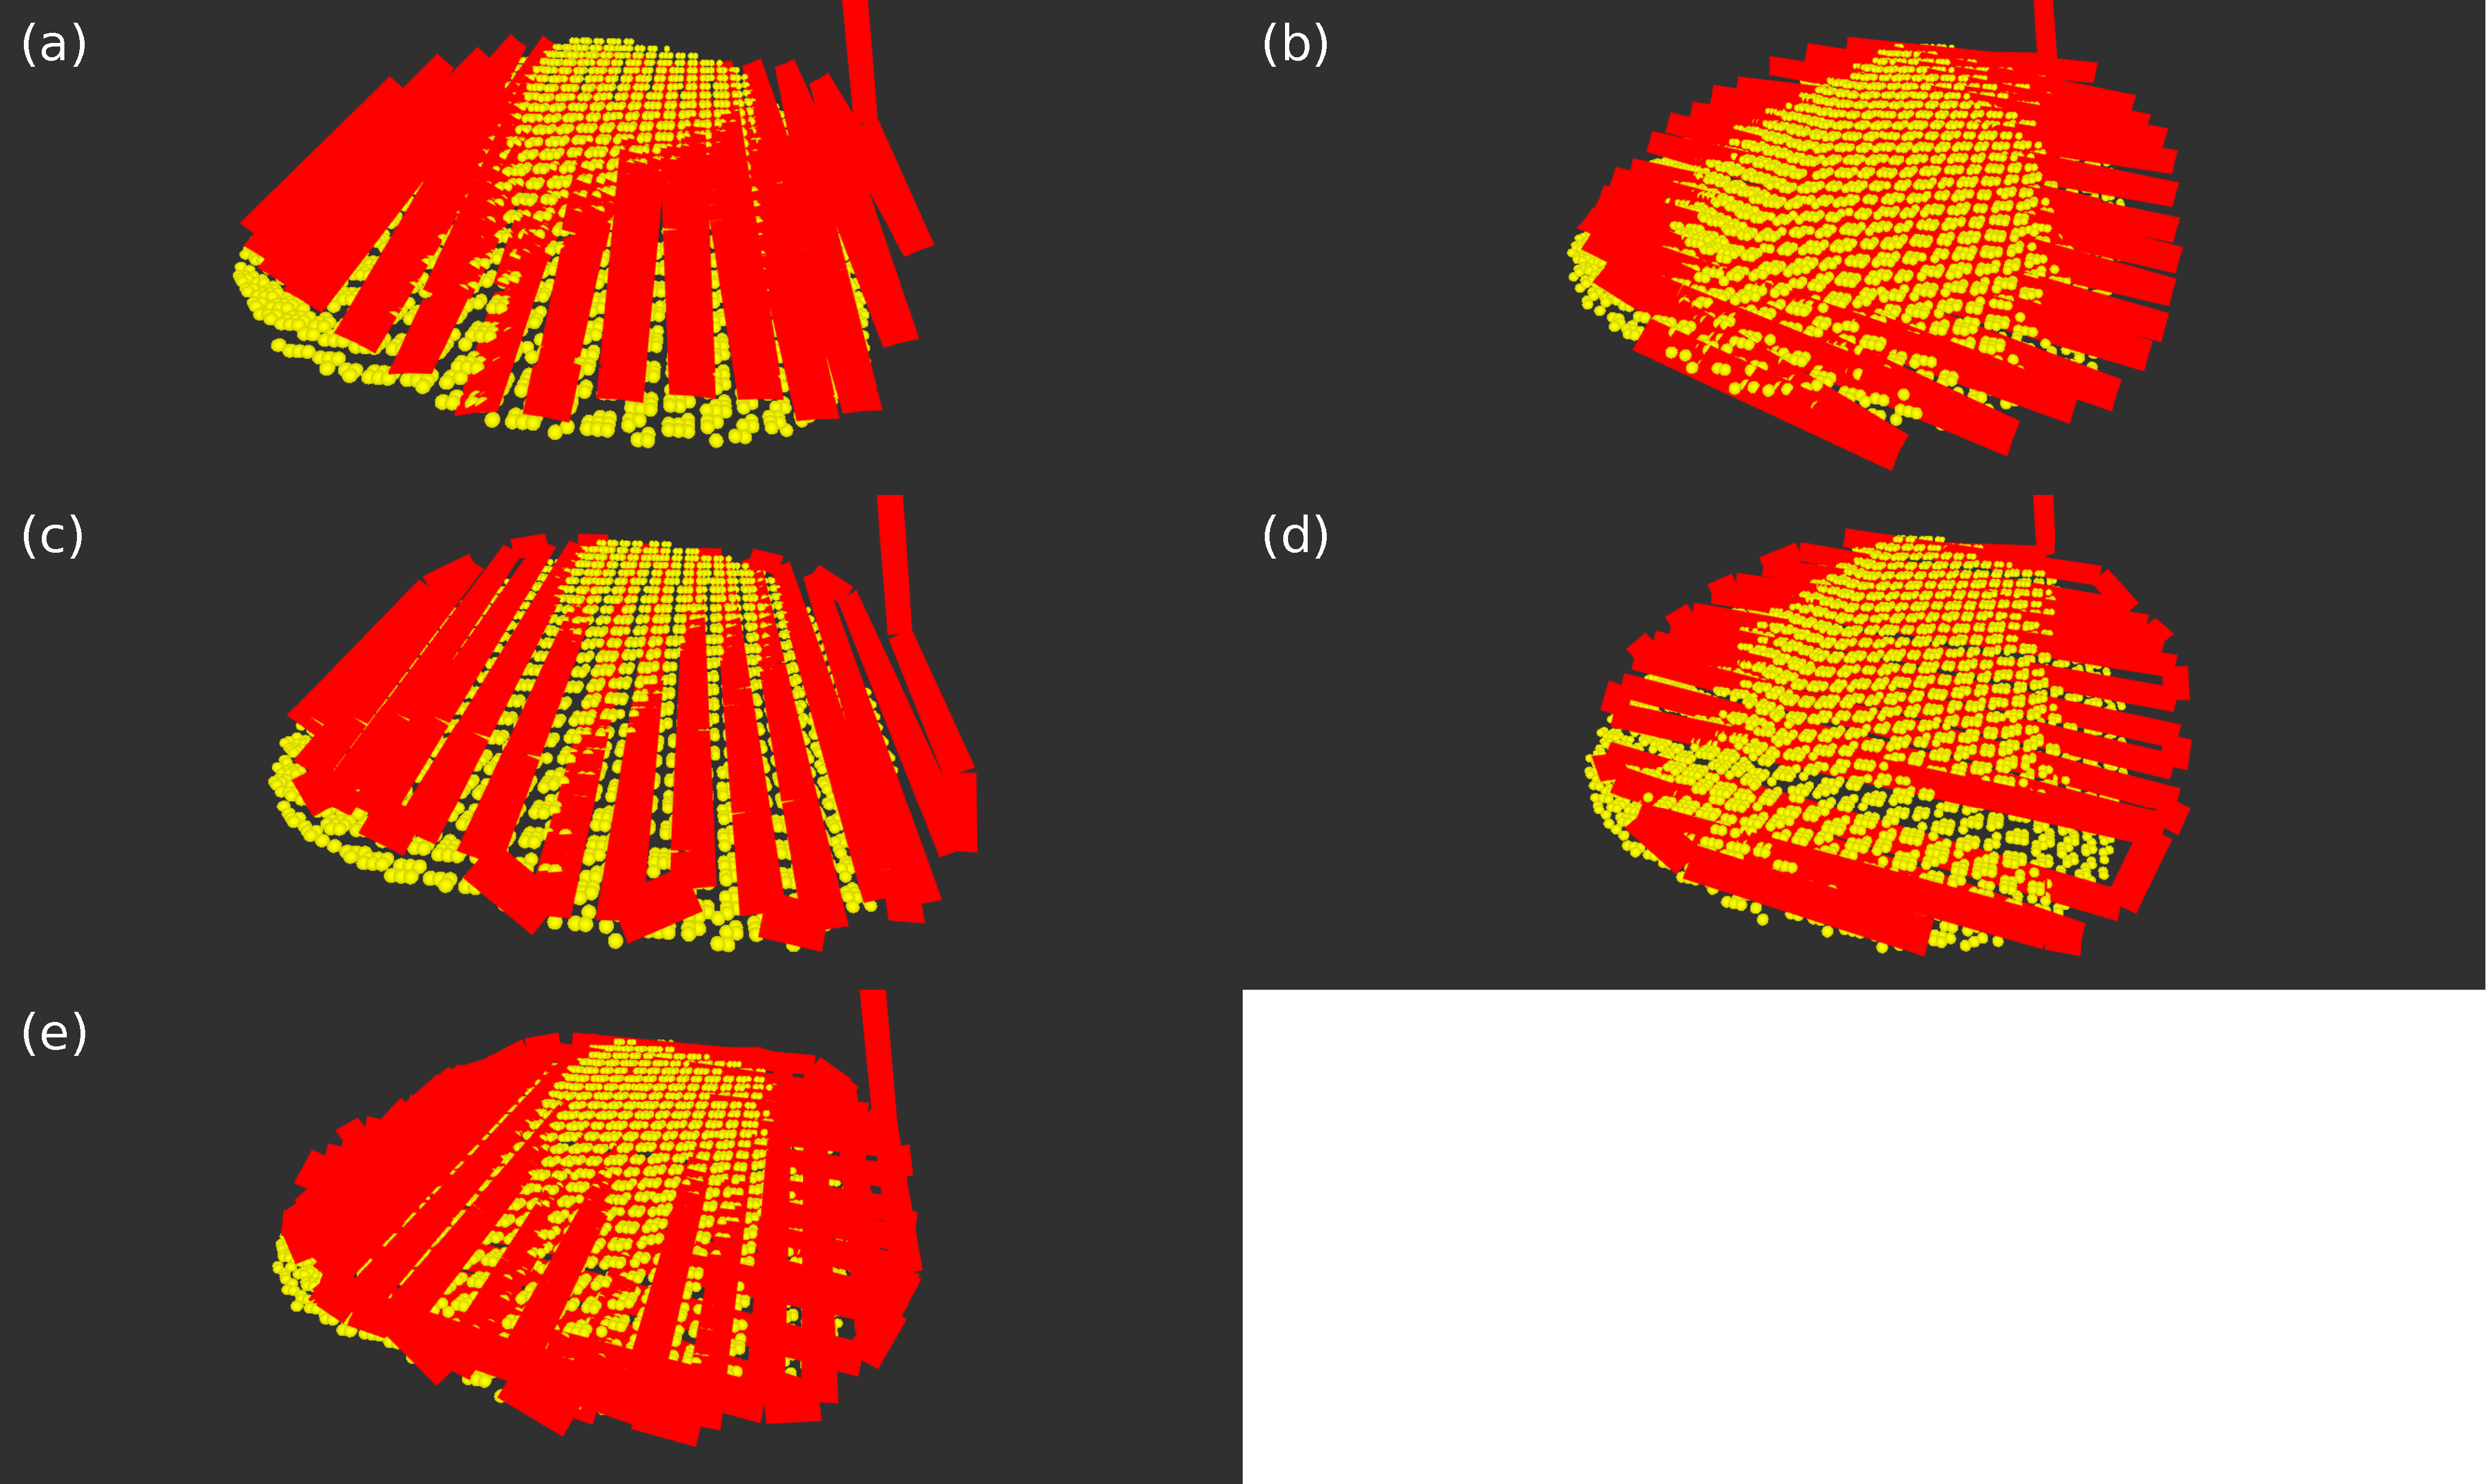
\includegraphics[width=\textwidth]{simulation_test_results_appendix_trajectory_wound_5}
	\caption[Wound 5 printing trajectory.]{Wound 5 printing trajectory. (a) ZigZag X, (b) ZigZag Y, (c) Parallel Lines X, (d) Parallel Lines Y, and (e) Grid path. All paths used $L = 5$.}
    \label{fig:simulation_test_results_appendix_trajectory_wound_5}
\end{figure}

% ------------------------
% Wound 1
% ------------------------

\begin{figure}[htbp]
	\centering
	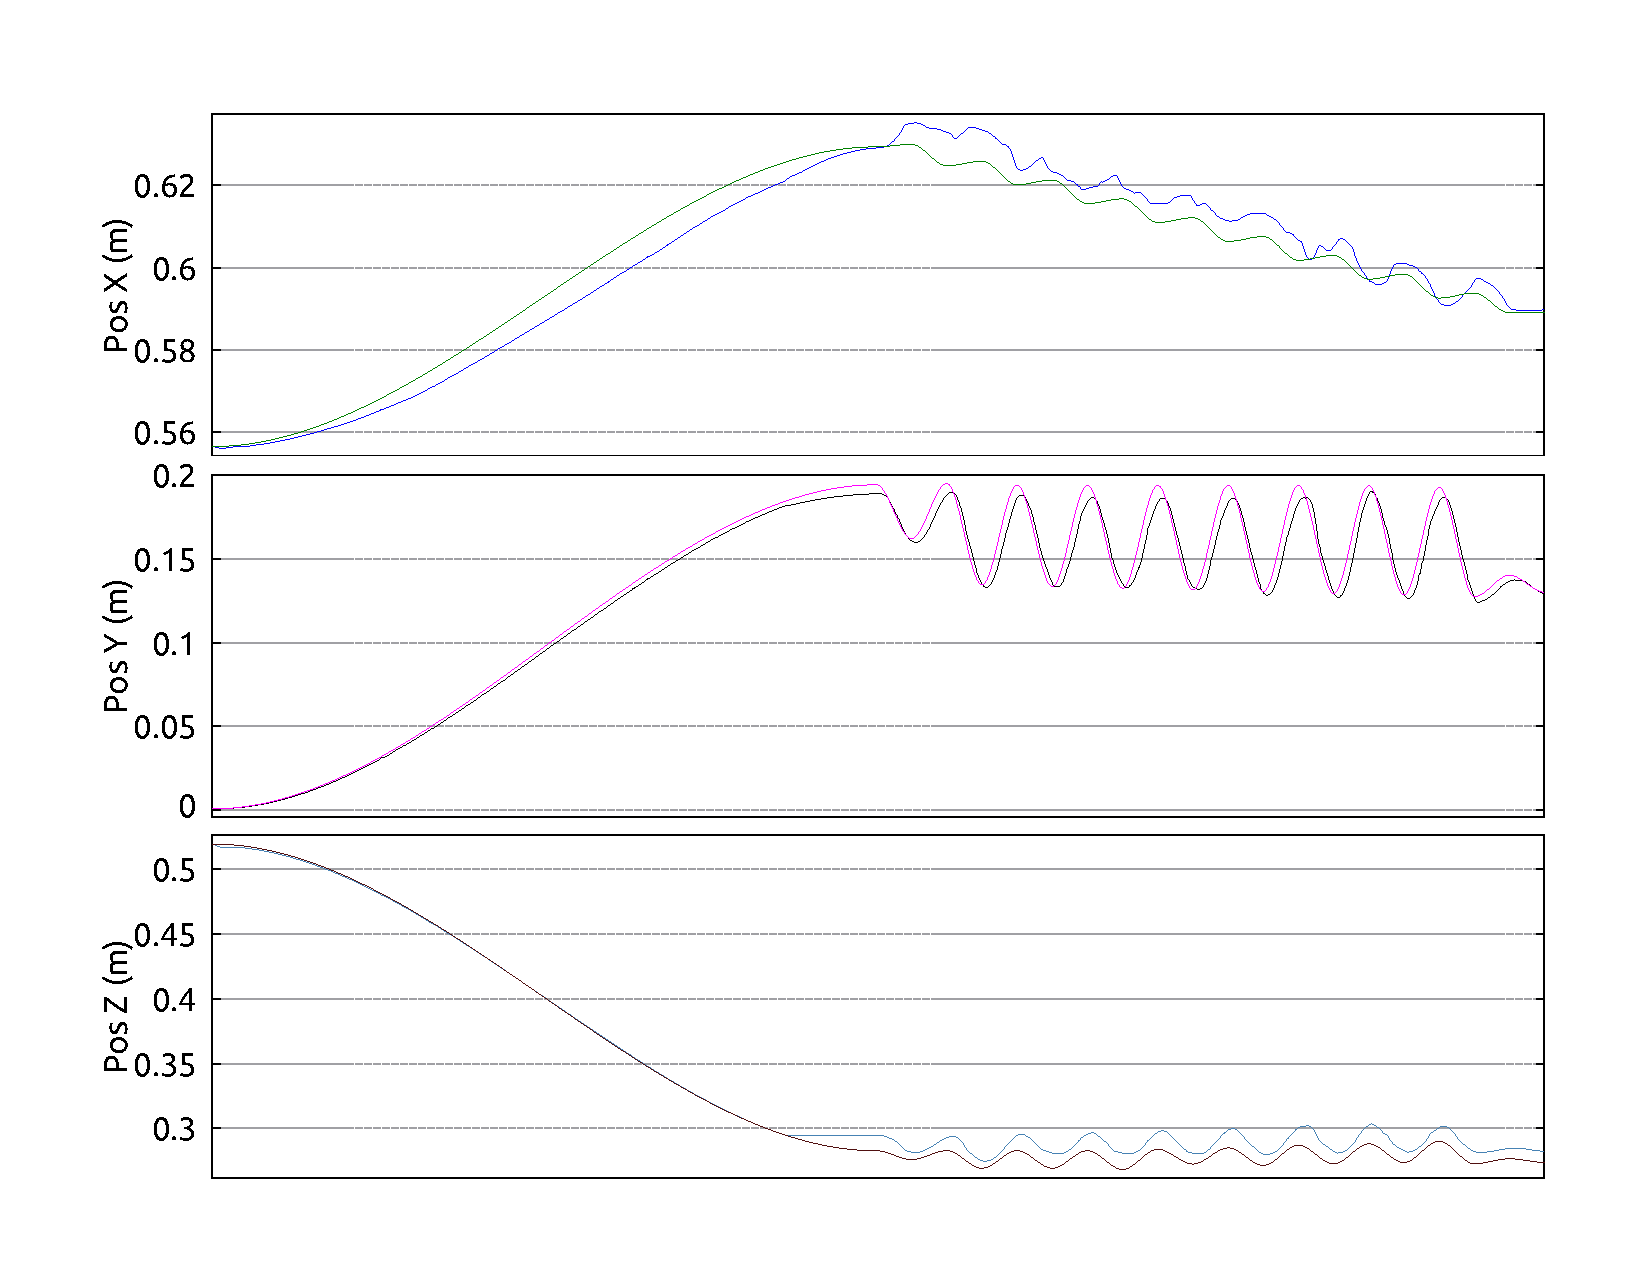
\includegraphics[width=\textwidth]{wound_0_zigzag_x_L5_20sec_position_track}
	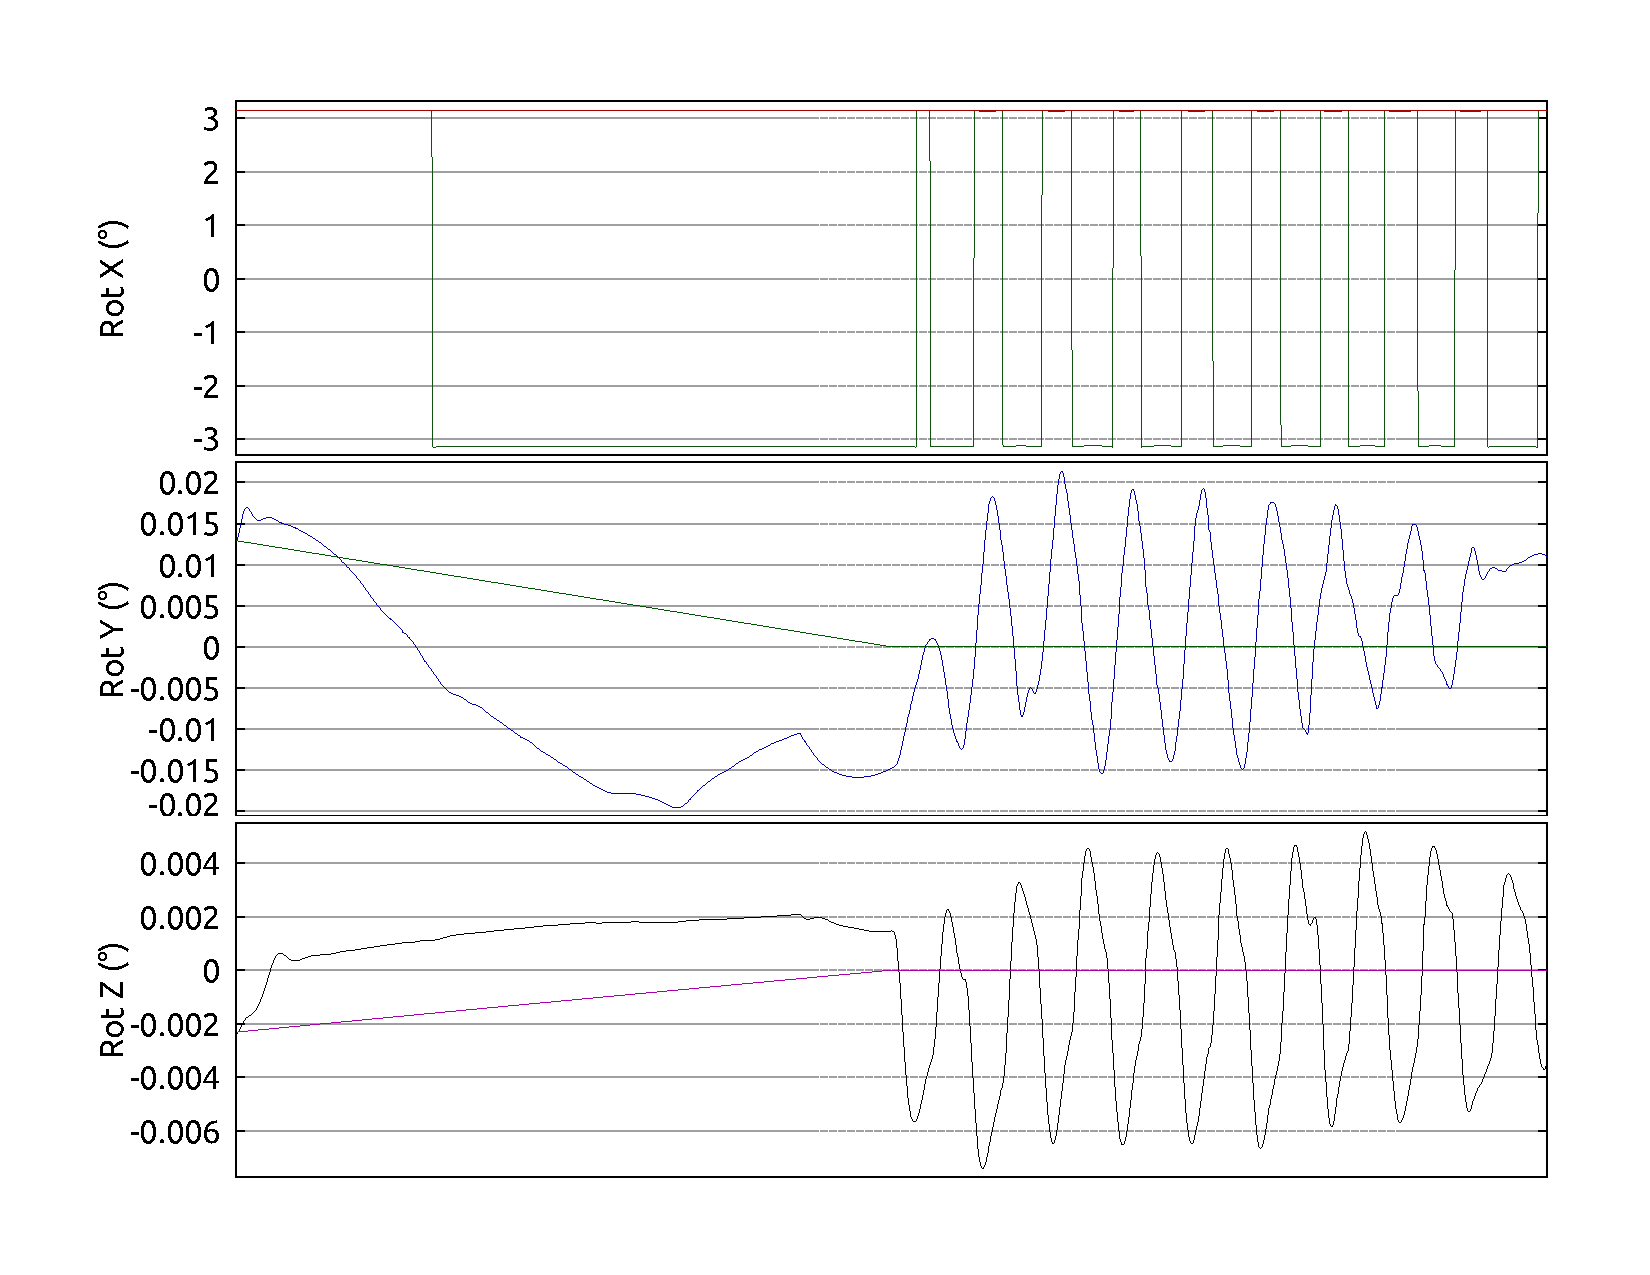
\includegraphics[width=\textwidth]{wound_0_zigzag_x_L5_20sec_orientation_track}
	\caption[Wound 1 printing trajectory tracking for ZigZag X path.]{Wound 1 printing trajectory tracking for ZigZag X path. (top) Position tracking. (bottom) Orientation tracking.}
    \label{fig:simulation_test_results_appendix_trajectory_tracking_wound_1_zizzag_x_tracking}
\end{figure}

\begin{figure}[htbp]
	\centering
	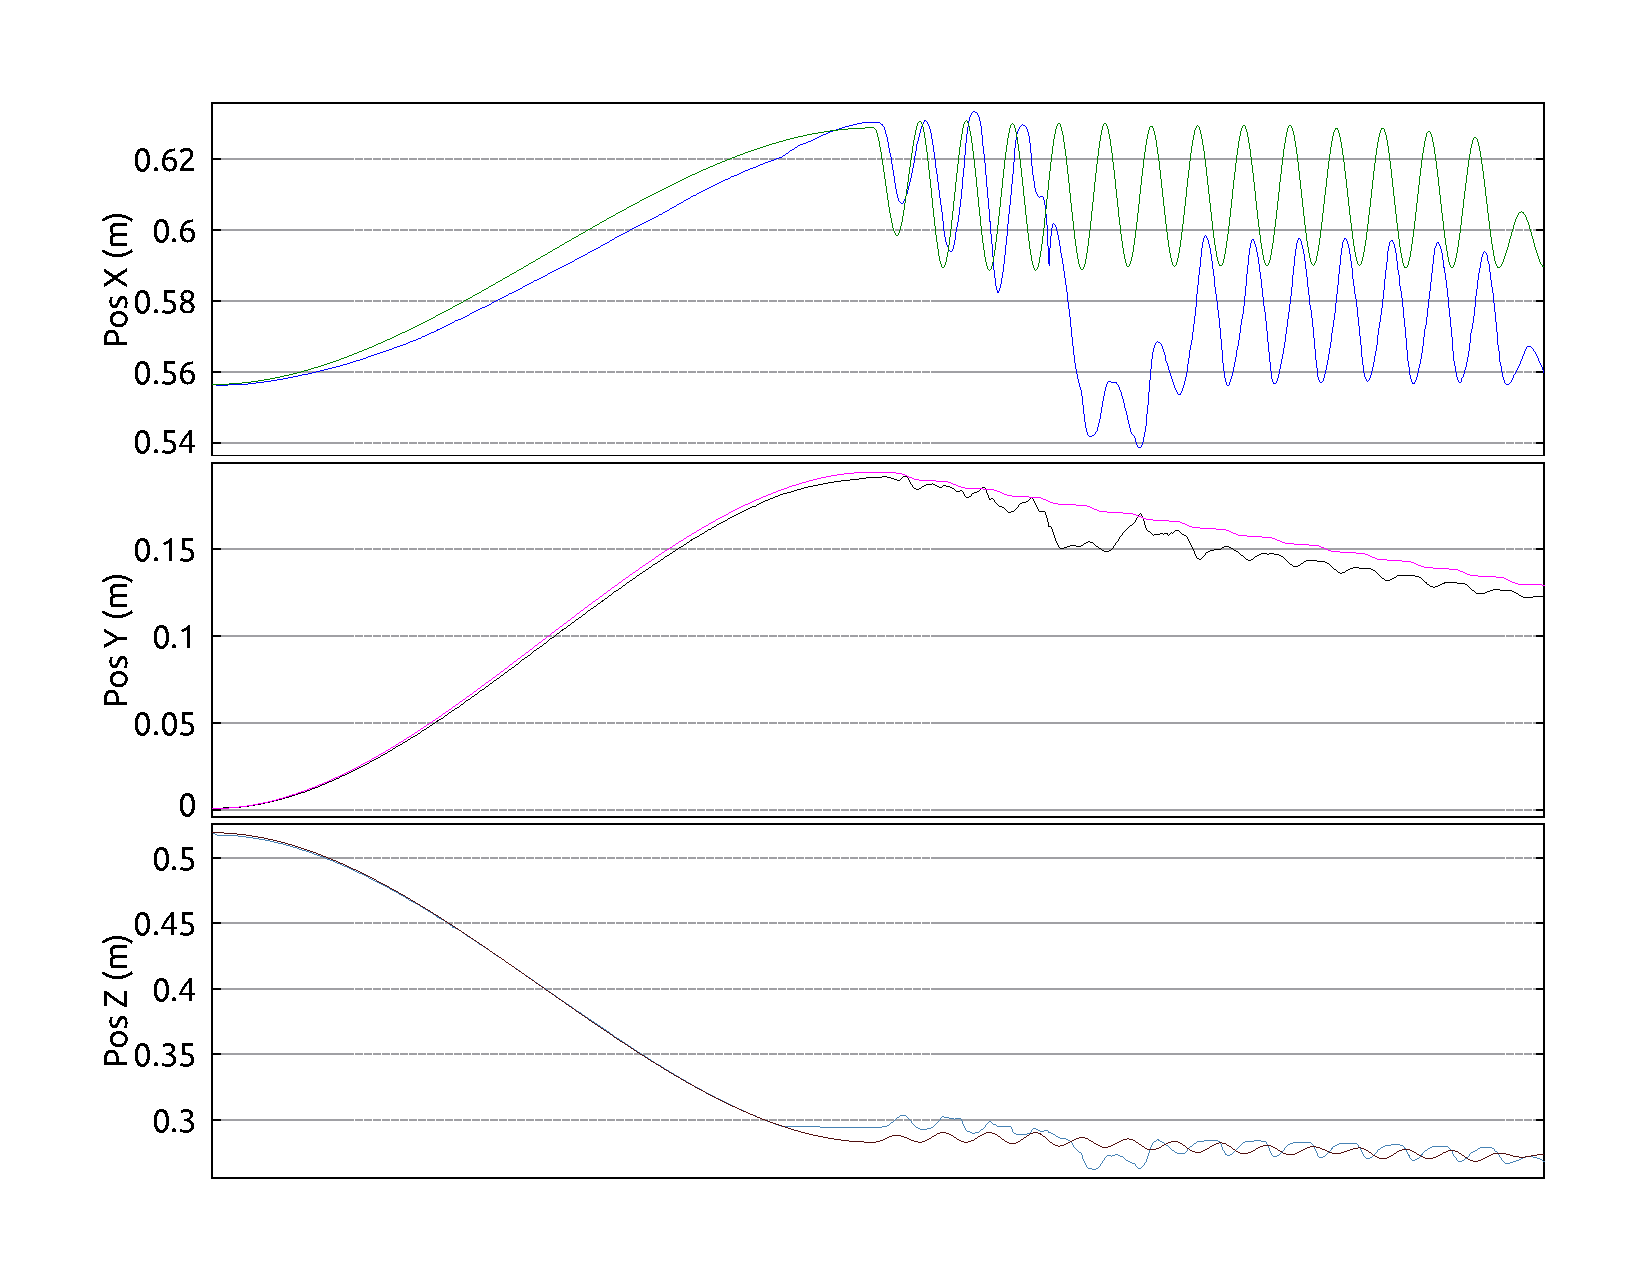
\includegraphics[width=\textwidth]{wound_0_zigzag_y_L5_20sec_position_track}
	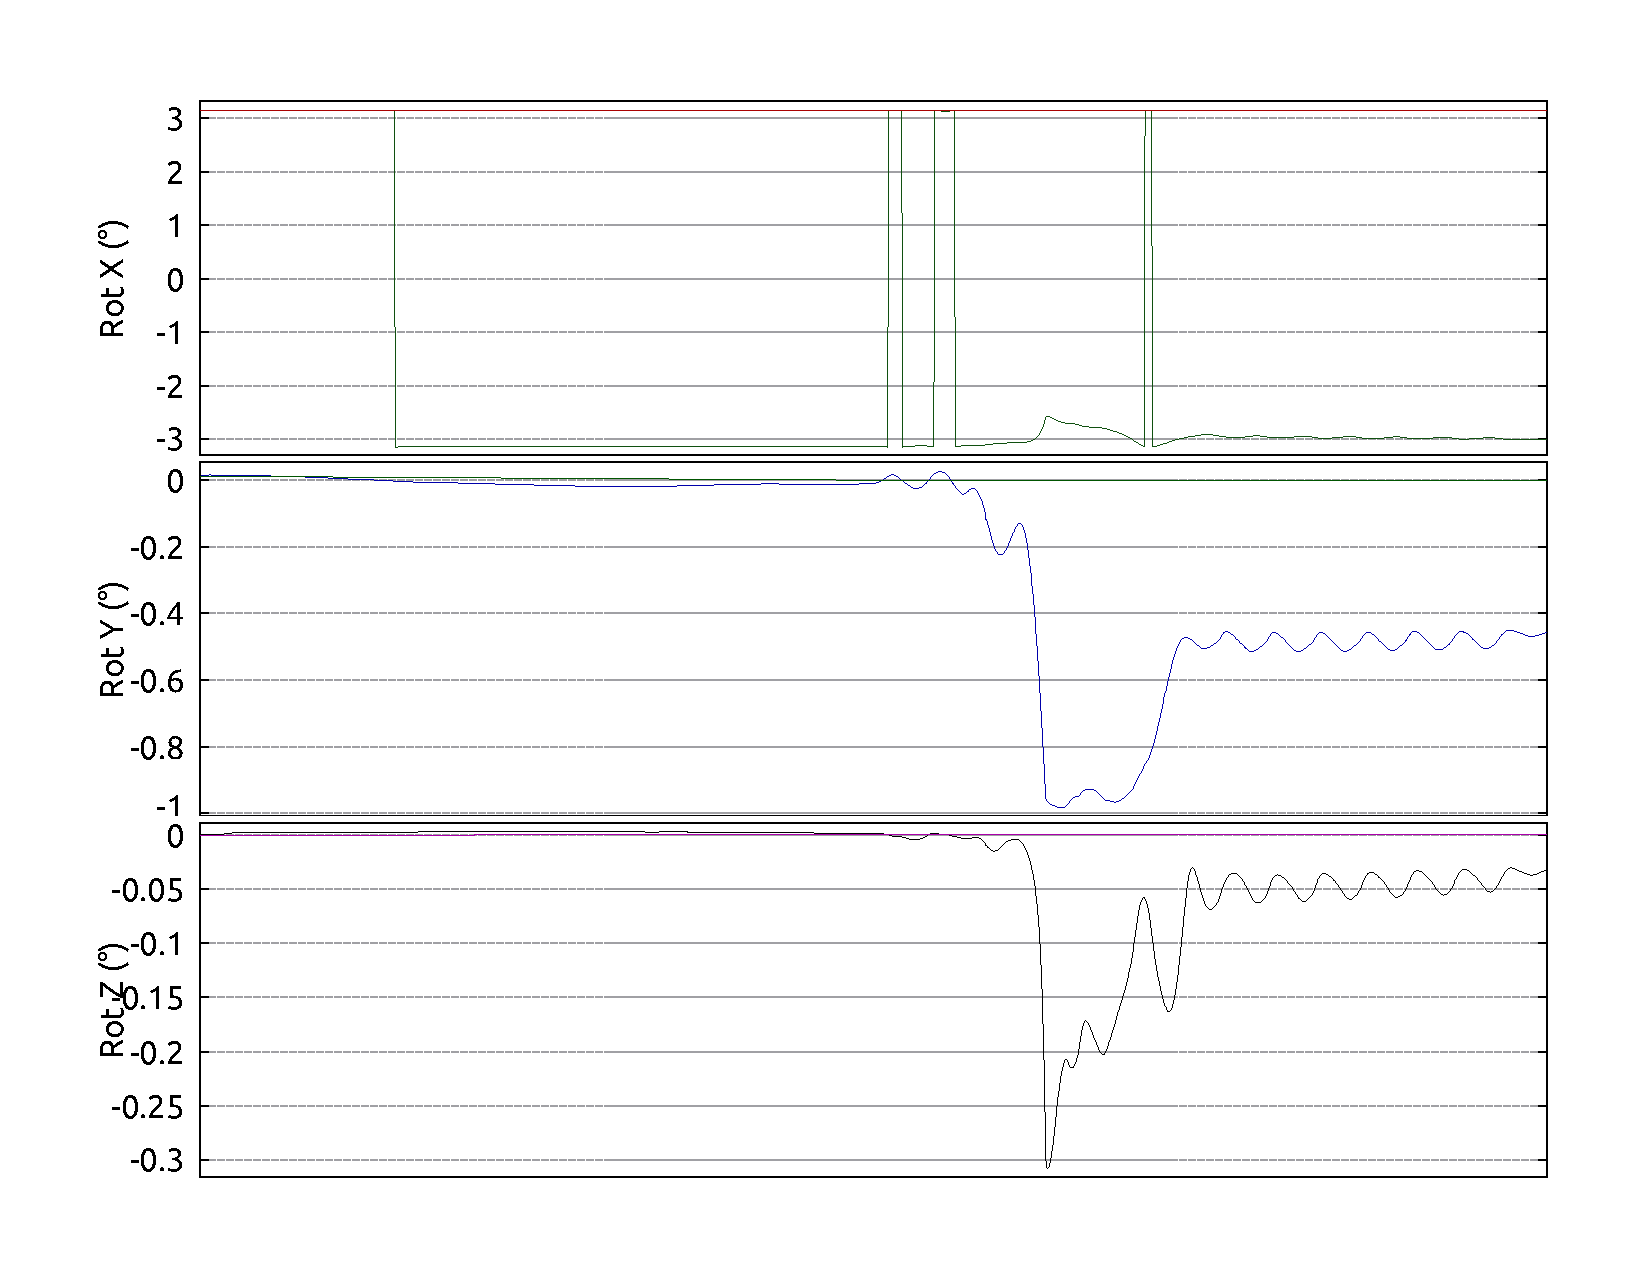
\includegraphics[width=\textwidth]{wound_0_zigzag_y_L5_20sec_orientation_track}
\caption[Wound 1 printing trajectory tracking for ZigZag Y path.]{Wound 1 printing trajectory tracking for ZigZag Y path. (top) Position tracking. (bottom) Orientation tracking.}
	\label{fig:simulation_test_results_appendix_trajectory_tracking_wound_1_zizzag_y_tracking}
\end{figure}

\begin{figure}[htbp]
	\centering
	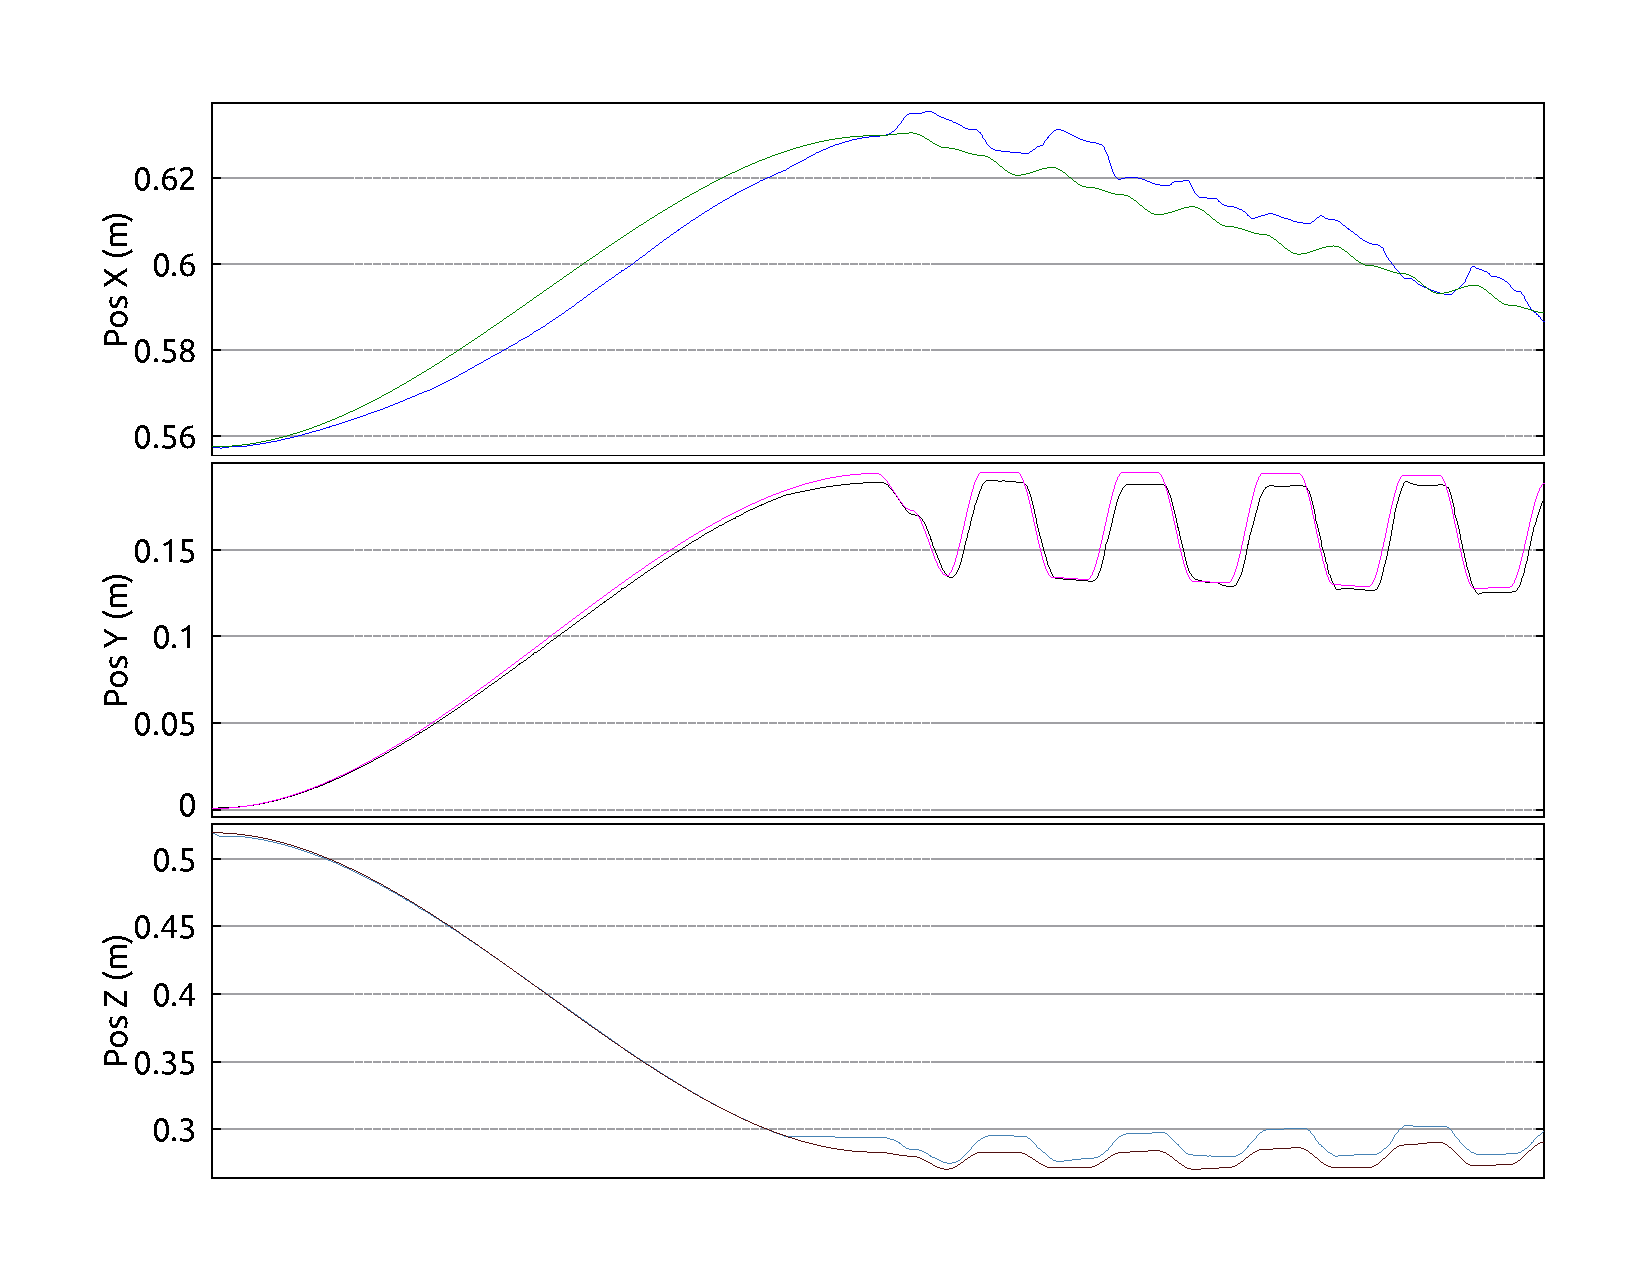
\includegraphics[width=\textwidth]{wound_0_parallel_x_L5_20sec_position_track}
	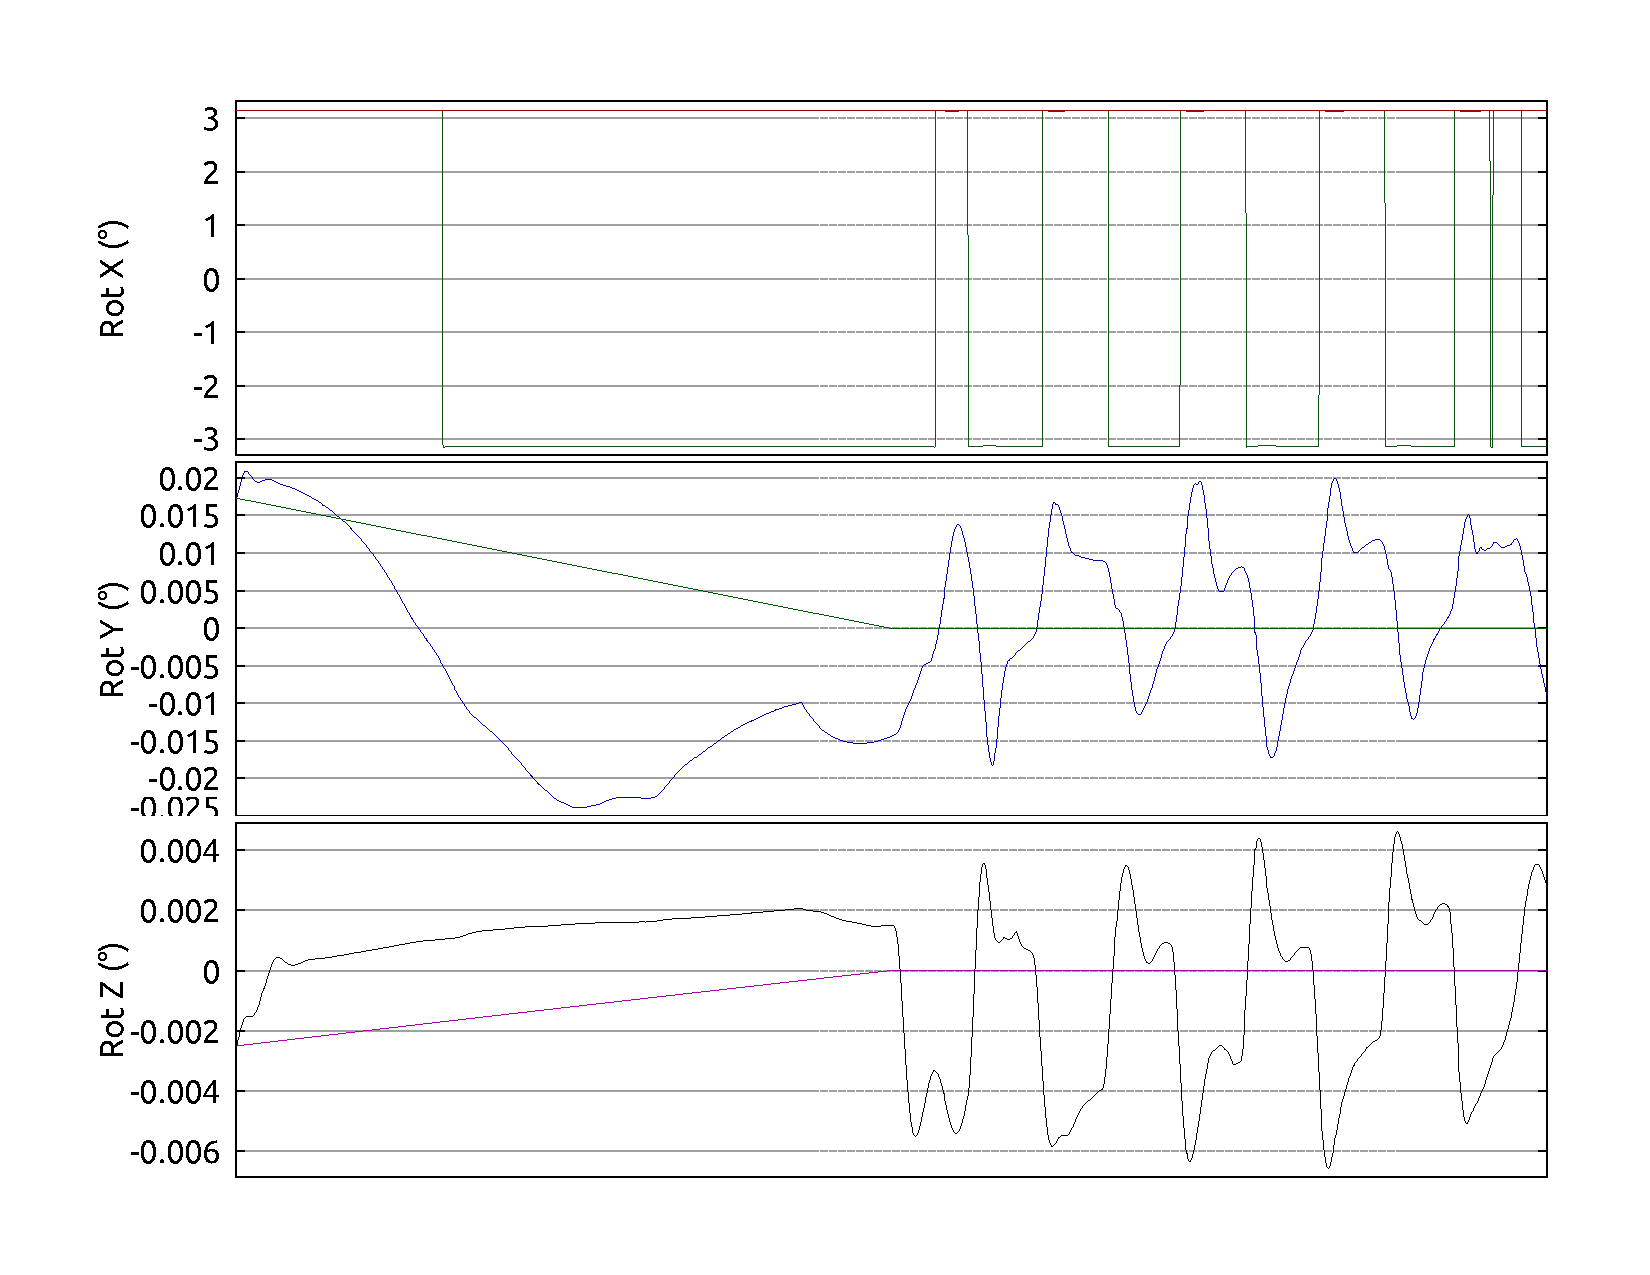
\includegraphics[width=\textwidth]{wound_0_parallel_x_L5_20sec_orientation_track}
	\caption[Wound 1 printing trajectory tracking for Parallel Lines X path.]{Wound 1 printing trajectory tracking for Parallel Lines X path. (top) Position tracking. (bottom) Orientation tracking.}
	\label{fig:simulation_test_results_appendix_trajectory_tracking_wound_1_parallel_x_tracking}
\end{figure}

\begin{figure}[htbp]
	\centering
	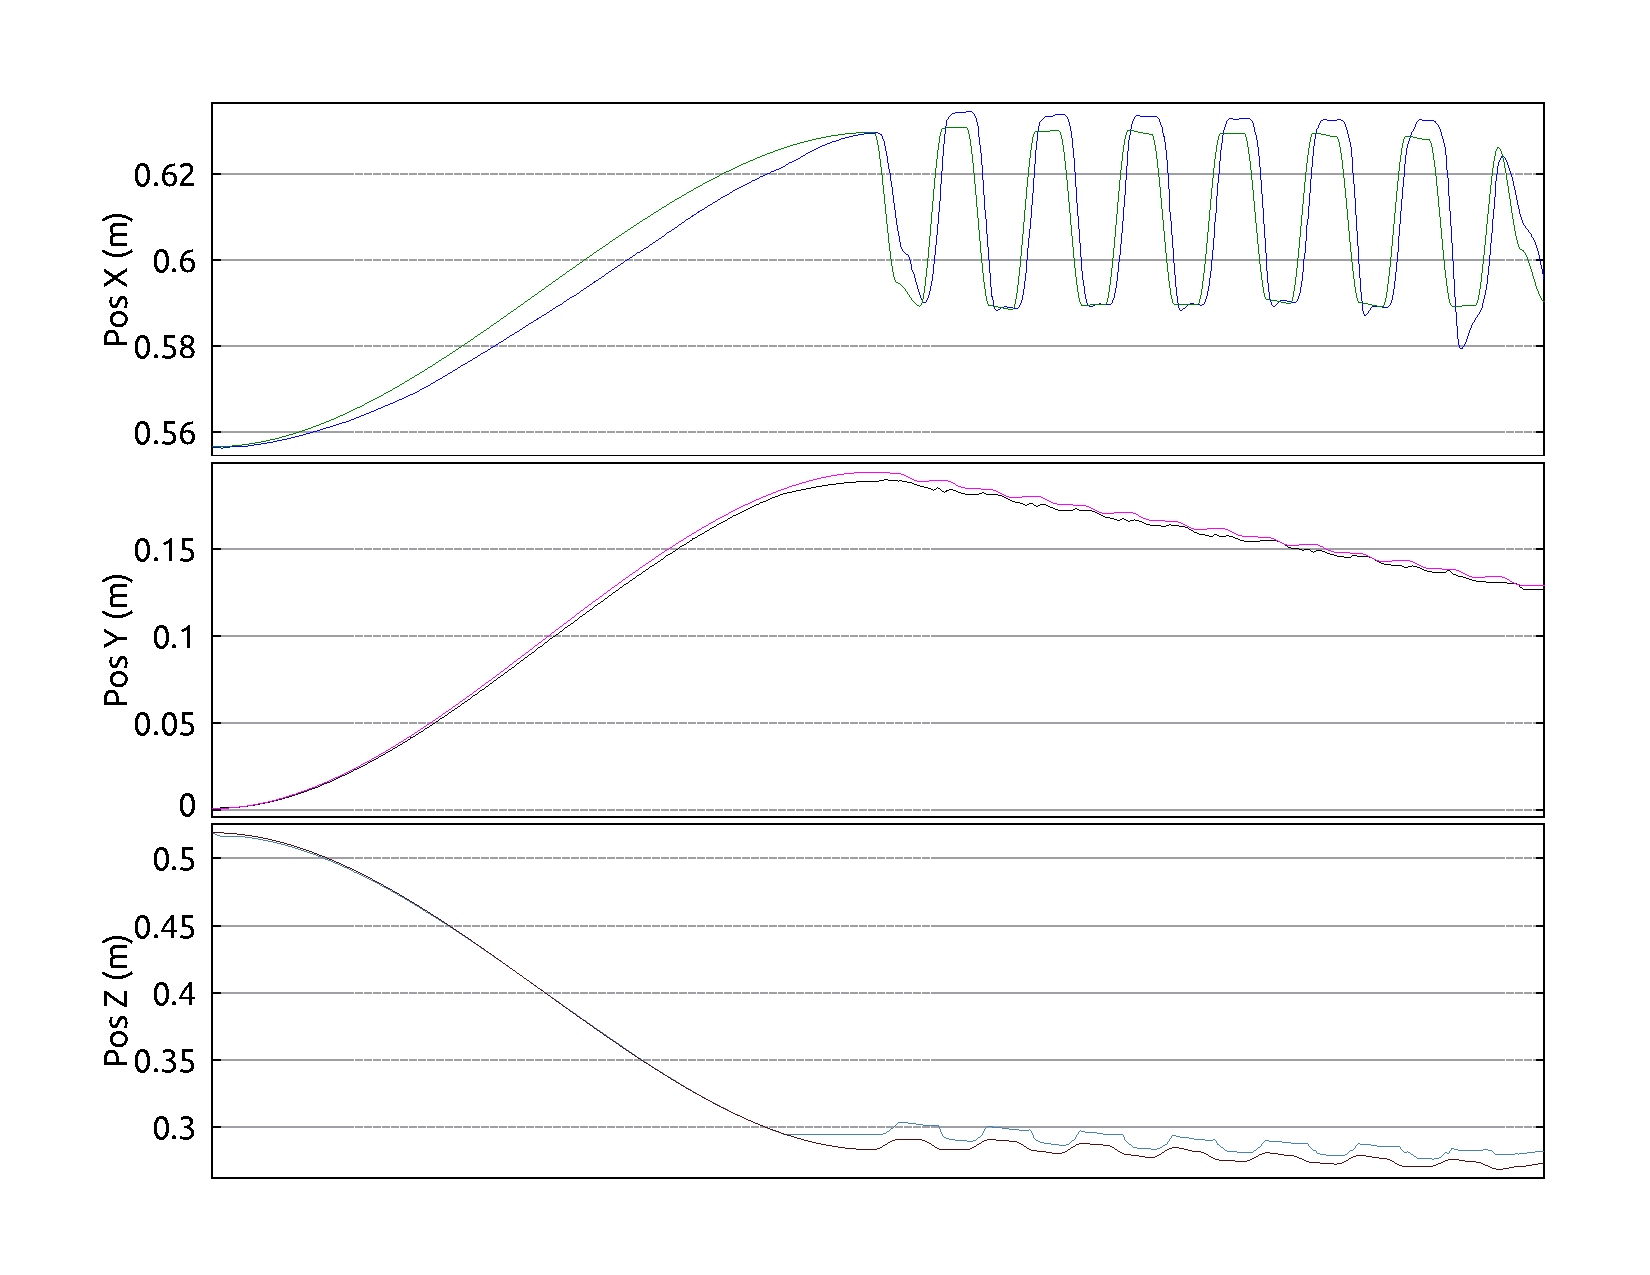
\includegraphics[width=\textwidth]{wound_0_parallel_y_L5_20sec_position_track}
	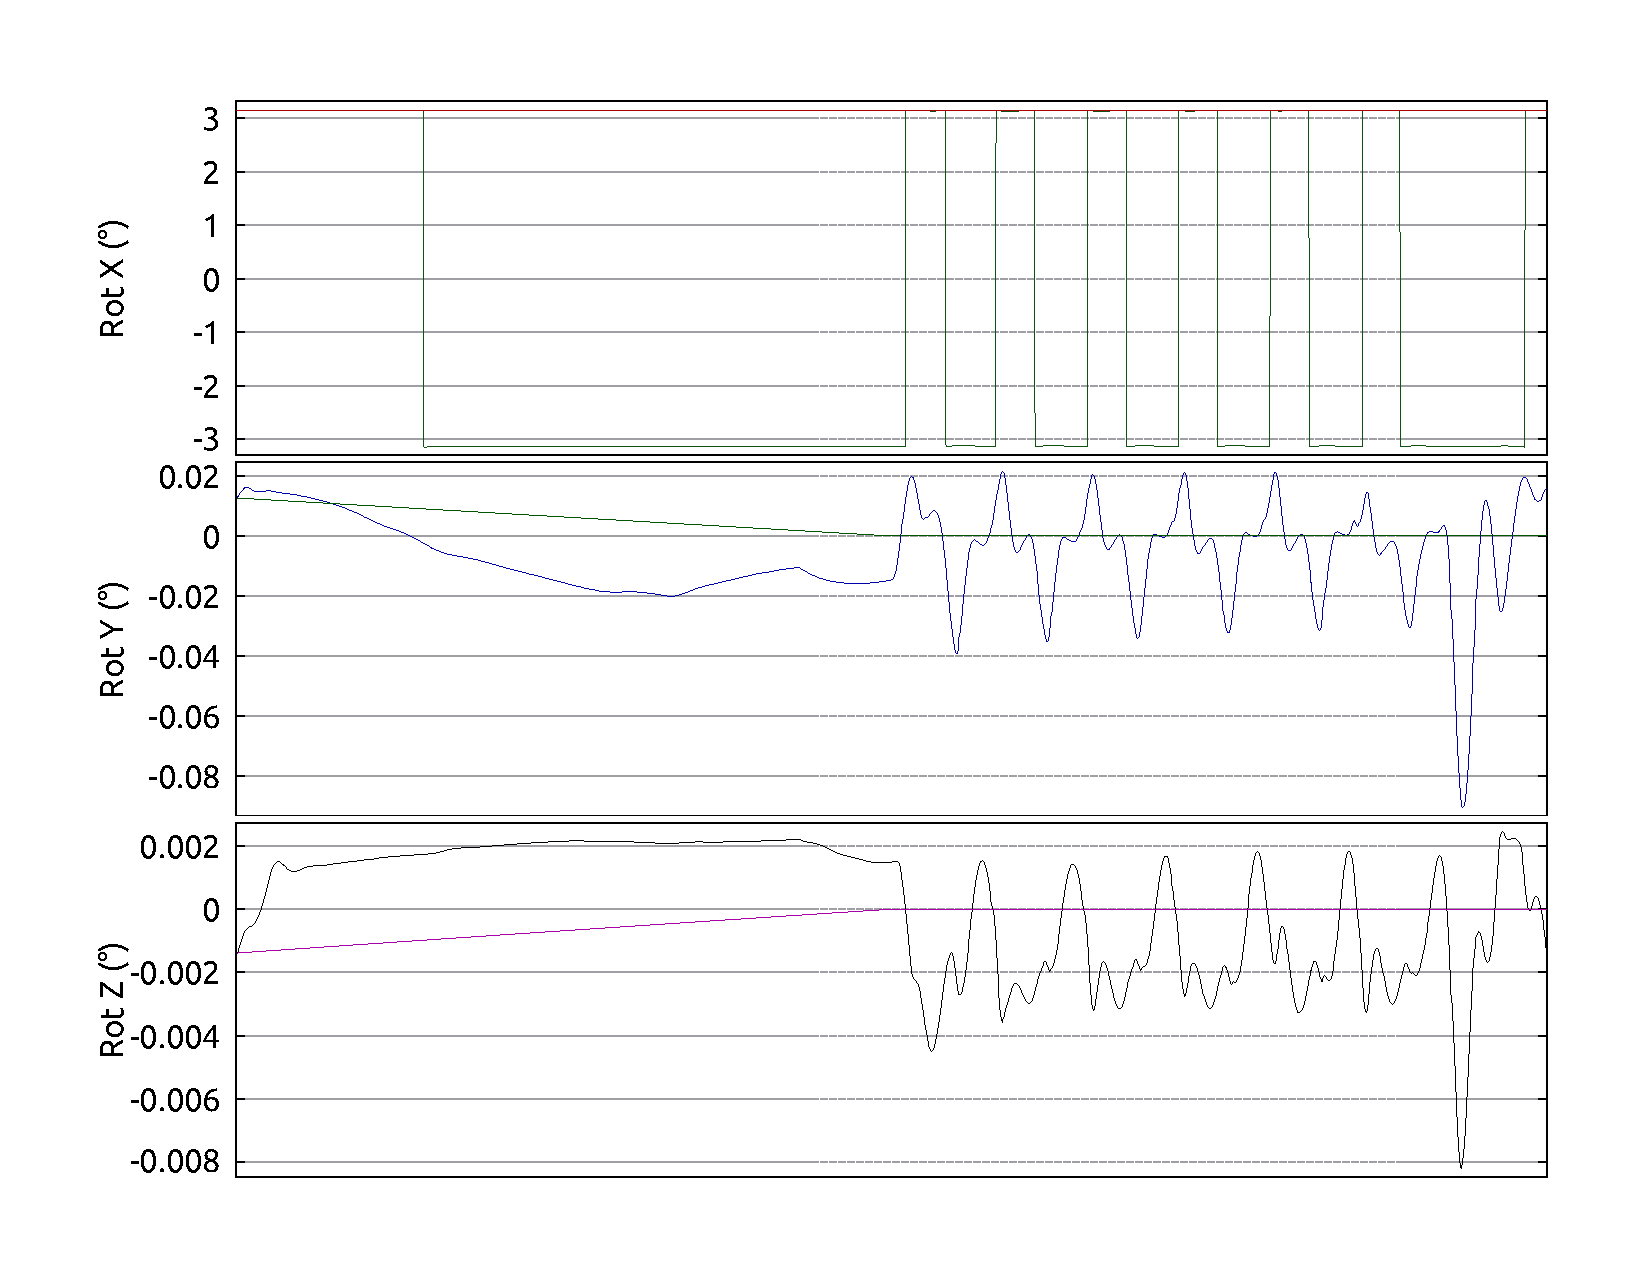
\includegraphics[width=\textwidth]{wound_0_parallel_y_L5_20sec_orientation_track}
    \caption[Wound 1 printing trajectory tracking for Parallel Lines Y path.]{Wound 1 printing trajectory tracking for Parallel Lines Y path. (top) Position tracking. (bottom) Orientation tracking.}
	\label{fig:simulation_test_results_appendix_trajectory_tracking_wound_1_parallel_y_tracking}
\end{figure}

\begin{figure}[htbp]
	\centering
	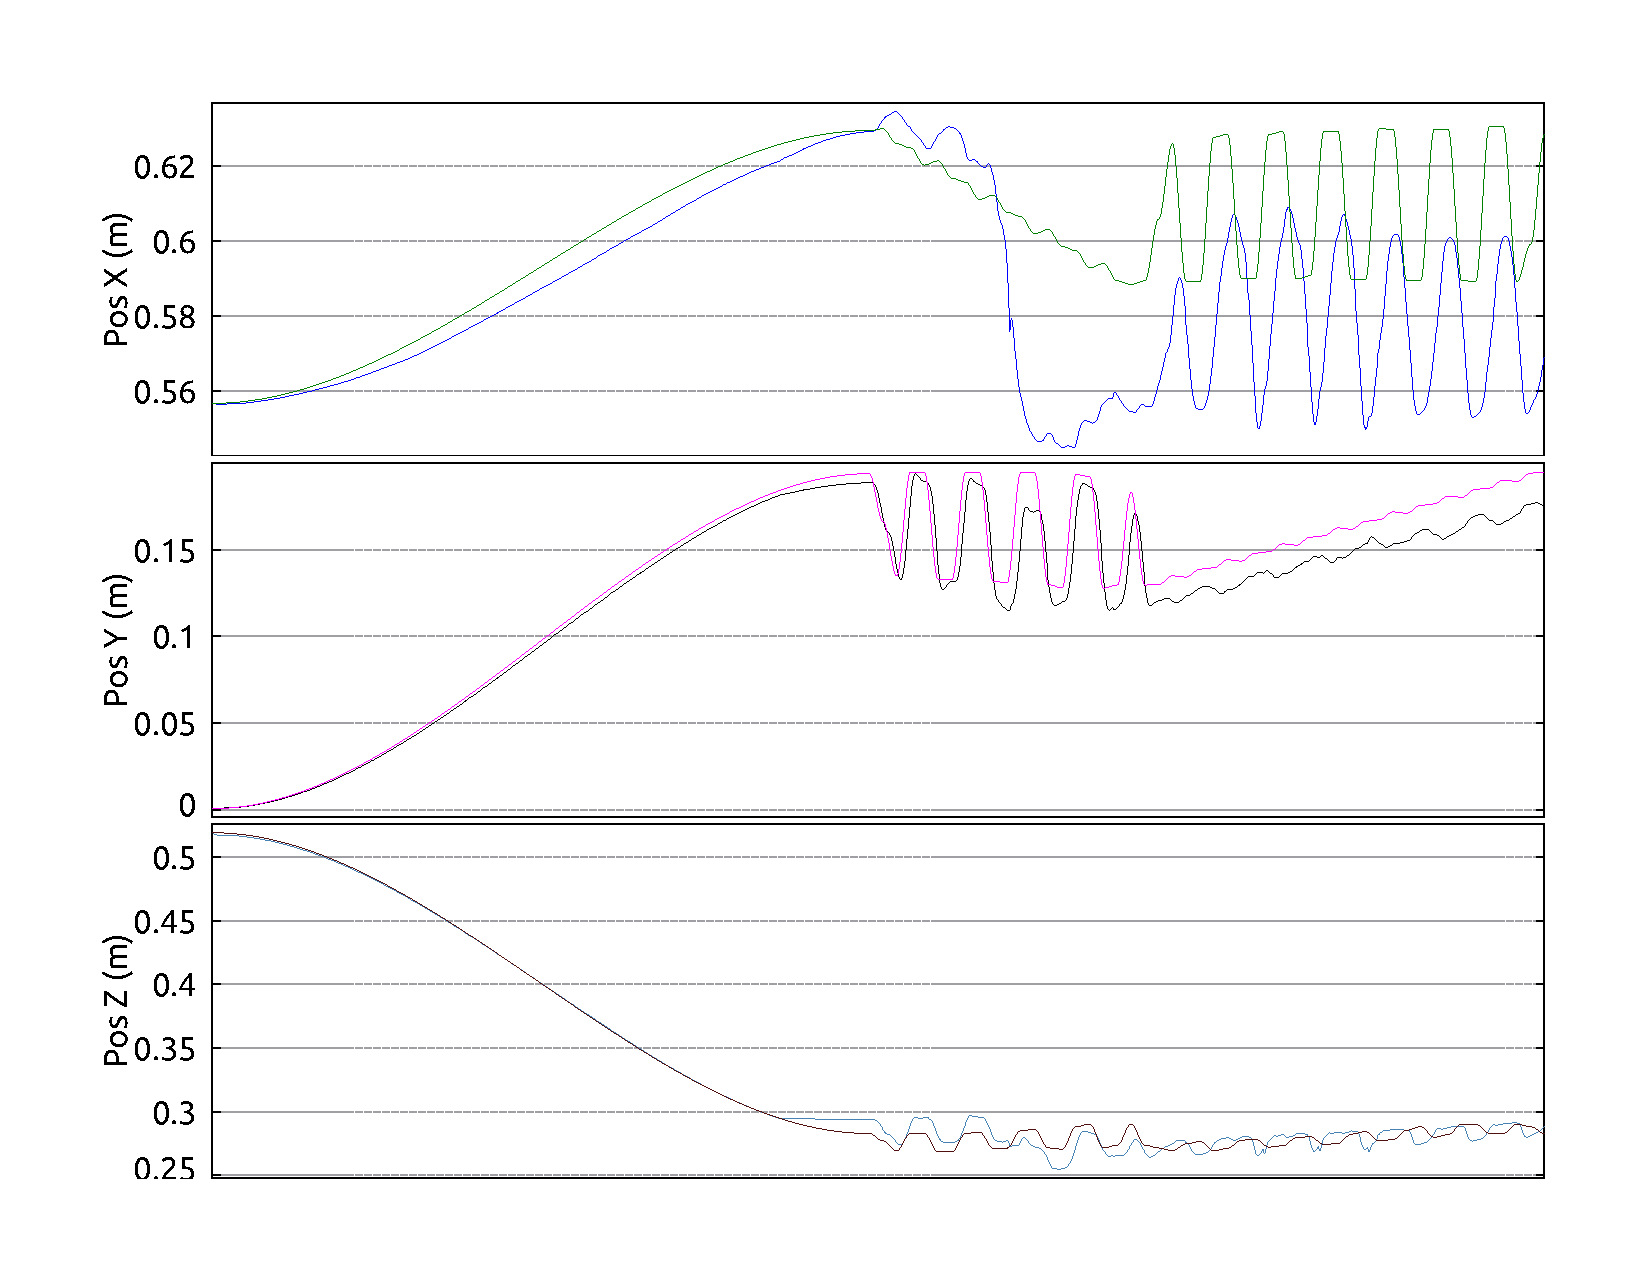
\includegraphics[width=\textwidth]{wound_0_grid_L5_20sec_position_track}
	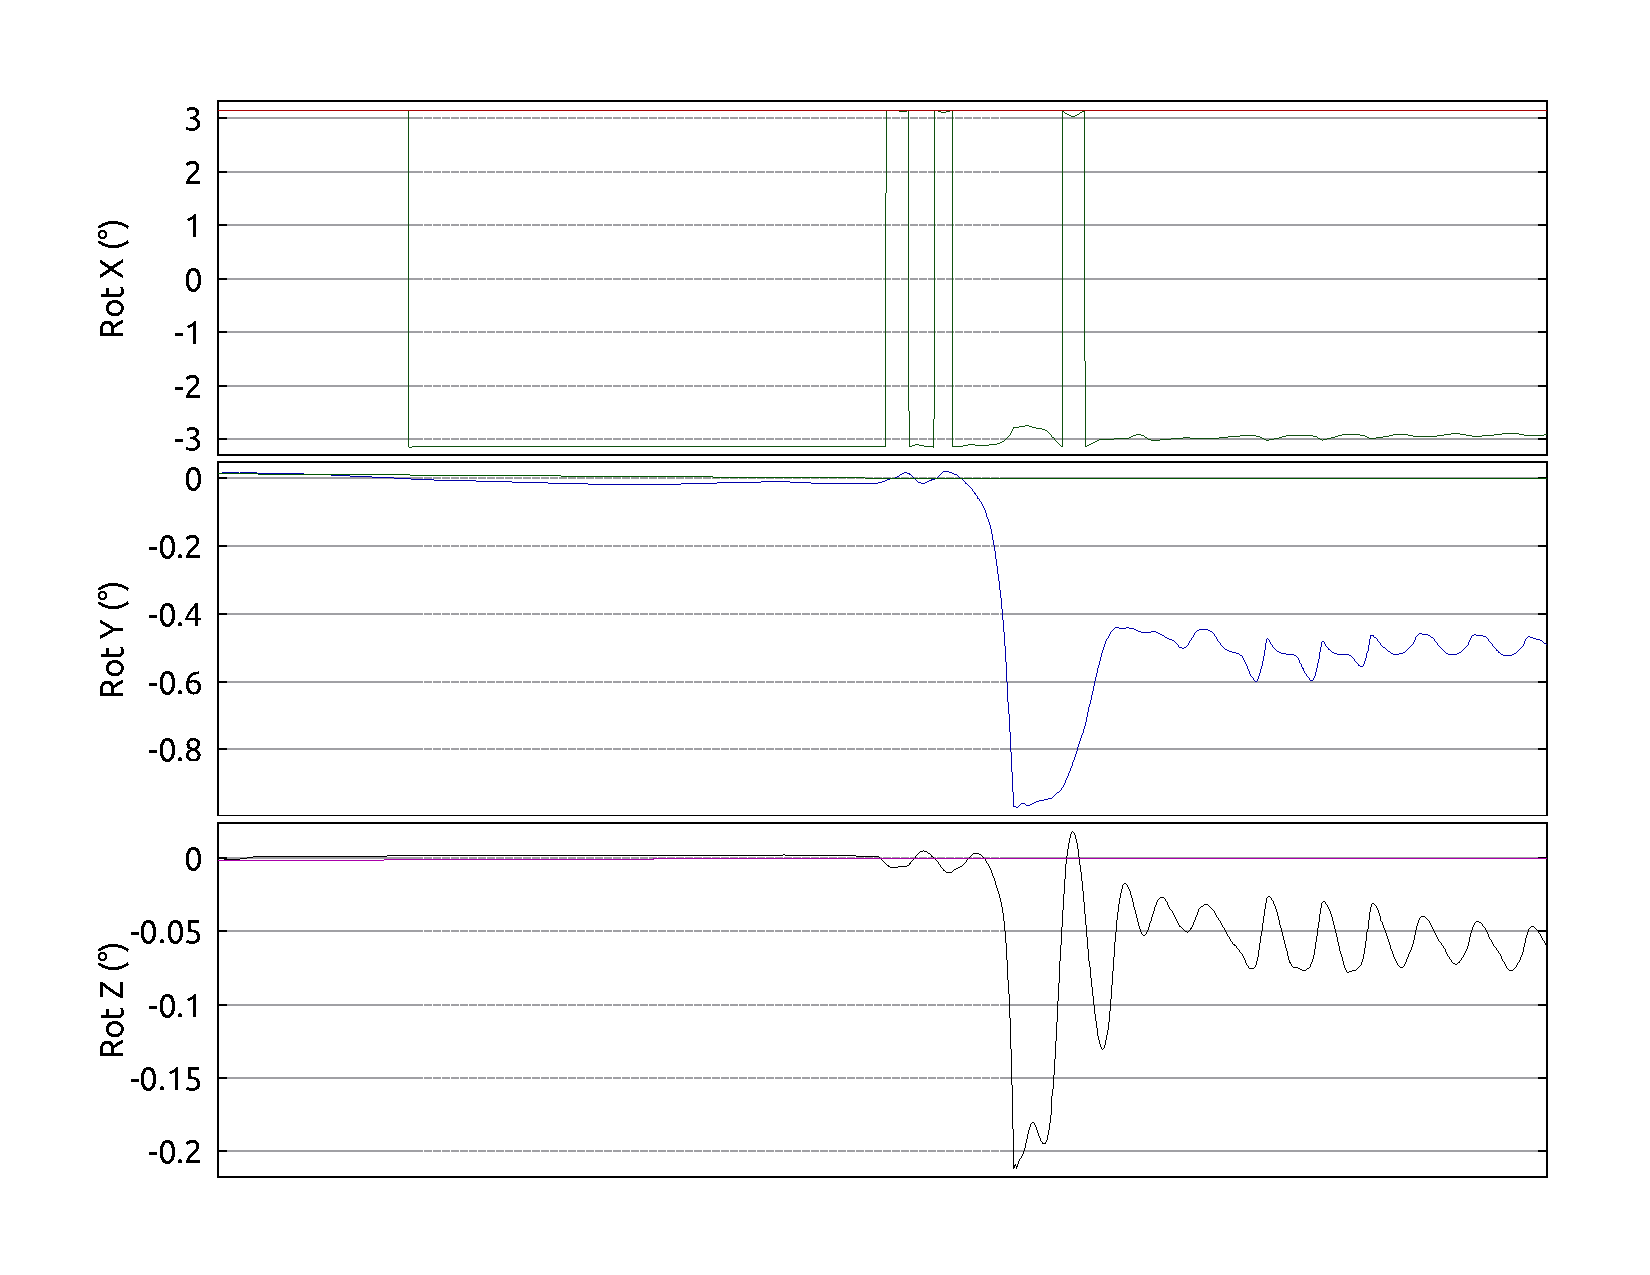
\includegraphics[width=\textwidth]{wound_0_grid_L5_20sec_orientation_track}
    \caption[Wound 1 printing trajectory tracking for Grid path.]{Wound 1 printing trajectory tracking for Grid path. (top) Position tracking. (bottom) Orientation tracking.}
	\label{fig:simulation_test_results_appendix_trajectory_tracking_wound_1_grid_tracking}
\end{figure}

% ------------------------
% Wound 2
% ------------------------

\begin{figure}[htbp]
	\centering
	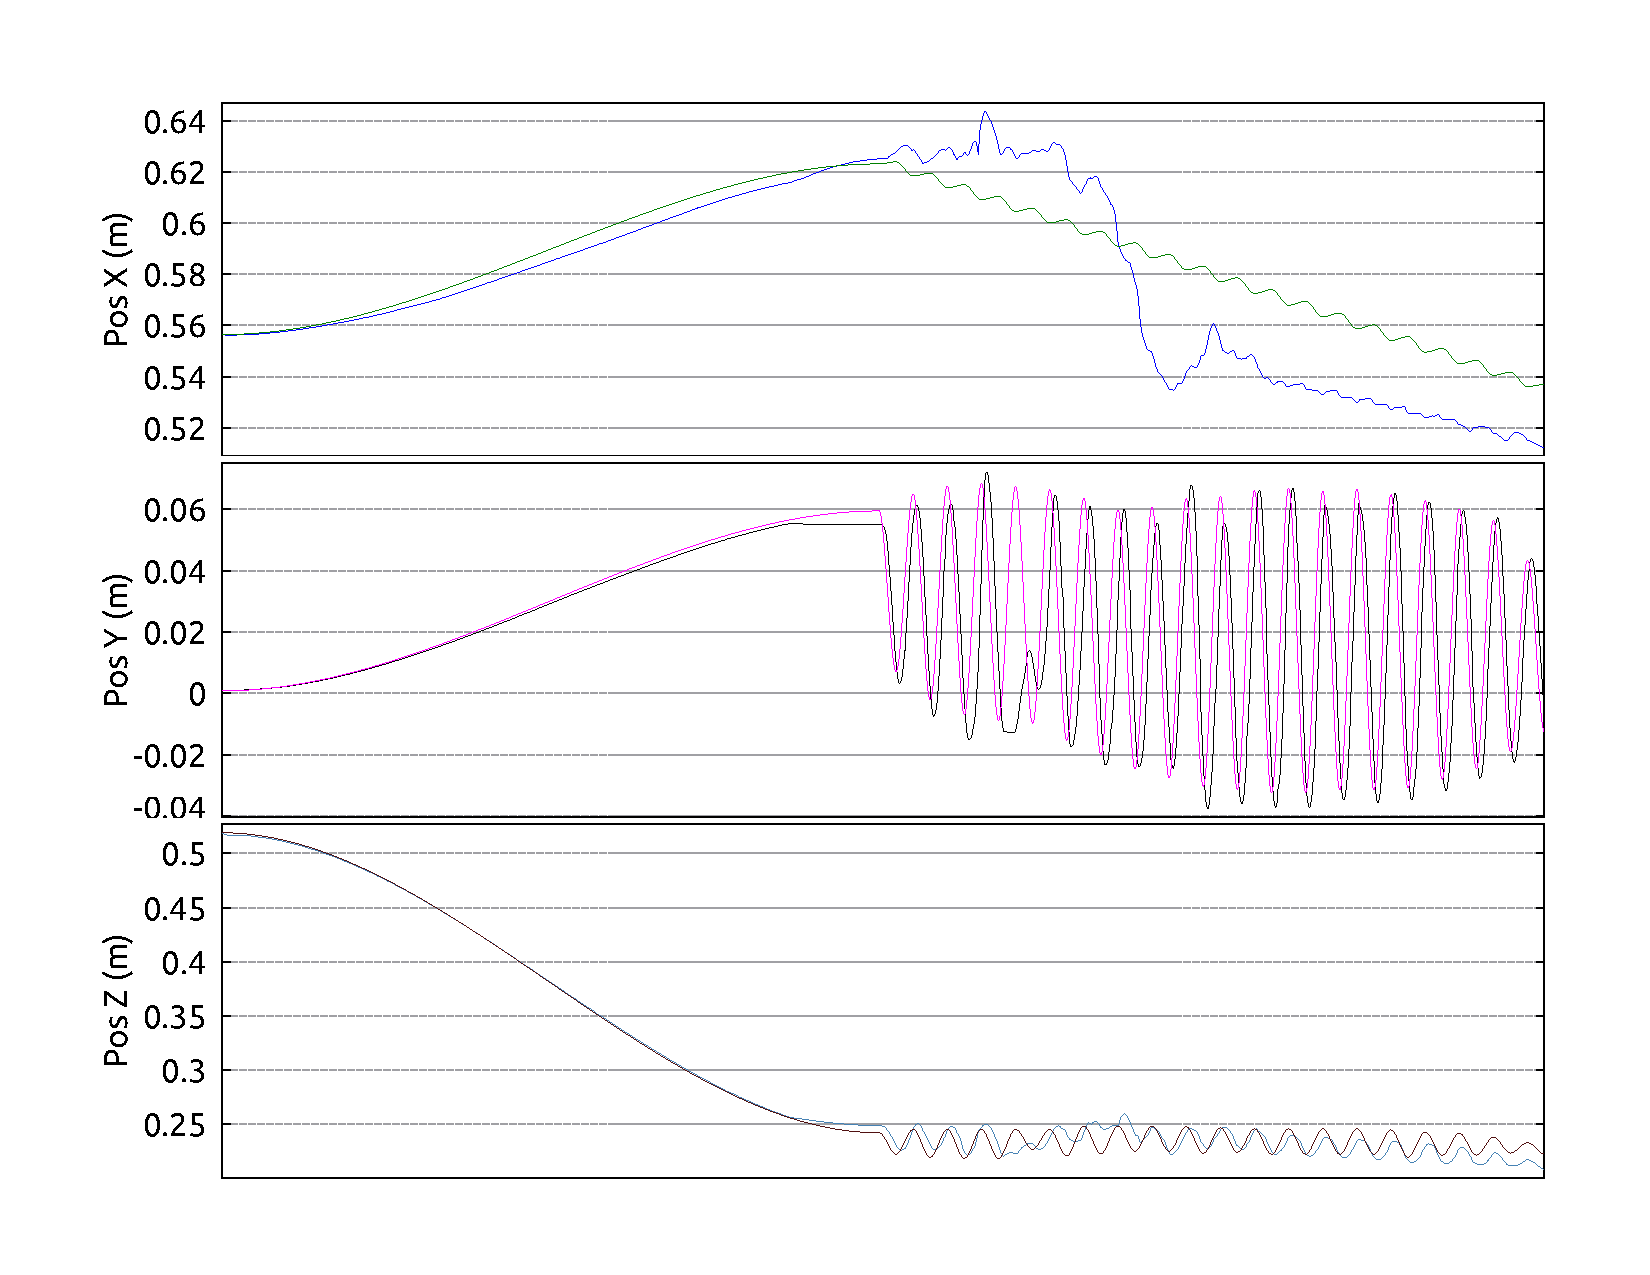
\includegraphics[width=\textwidth]{wound_1_zigzag_x_L5_20sec_position_track}
	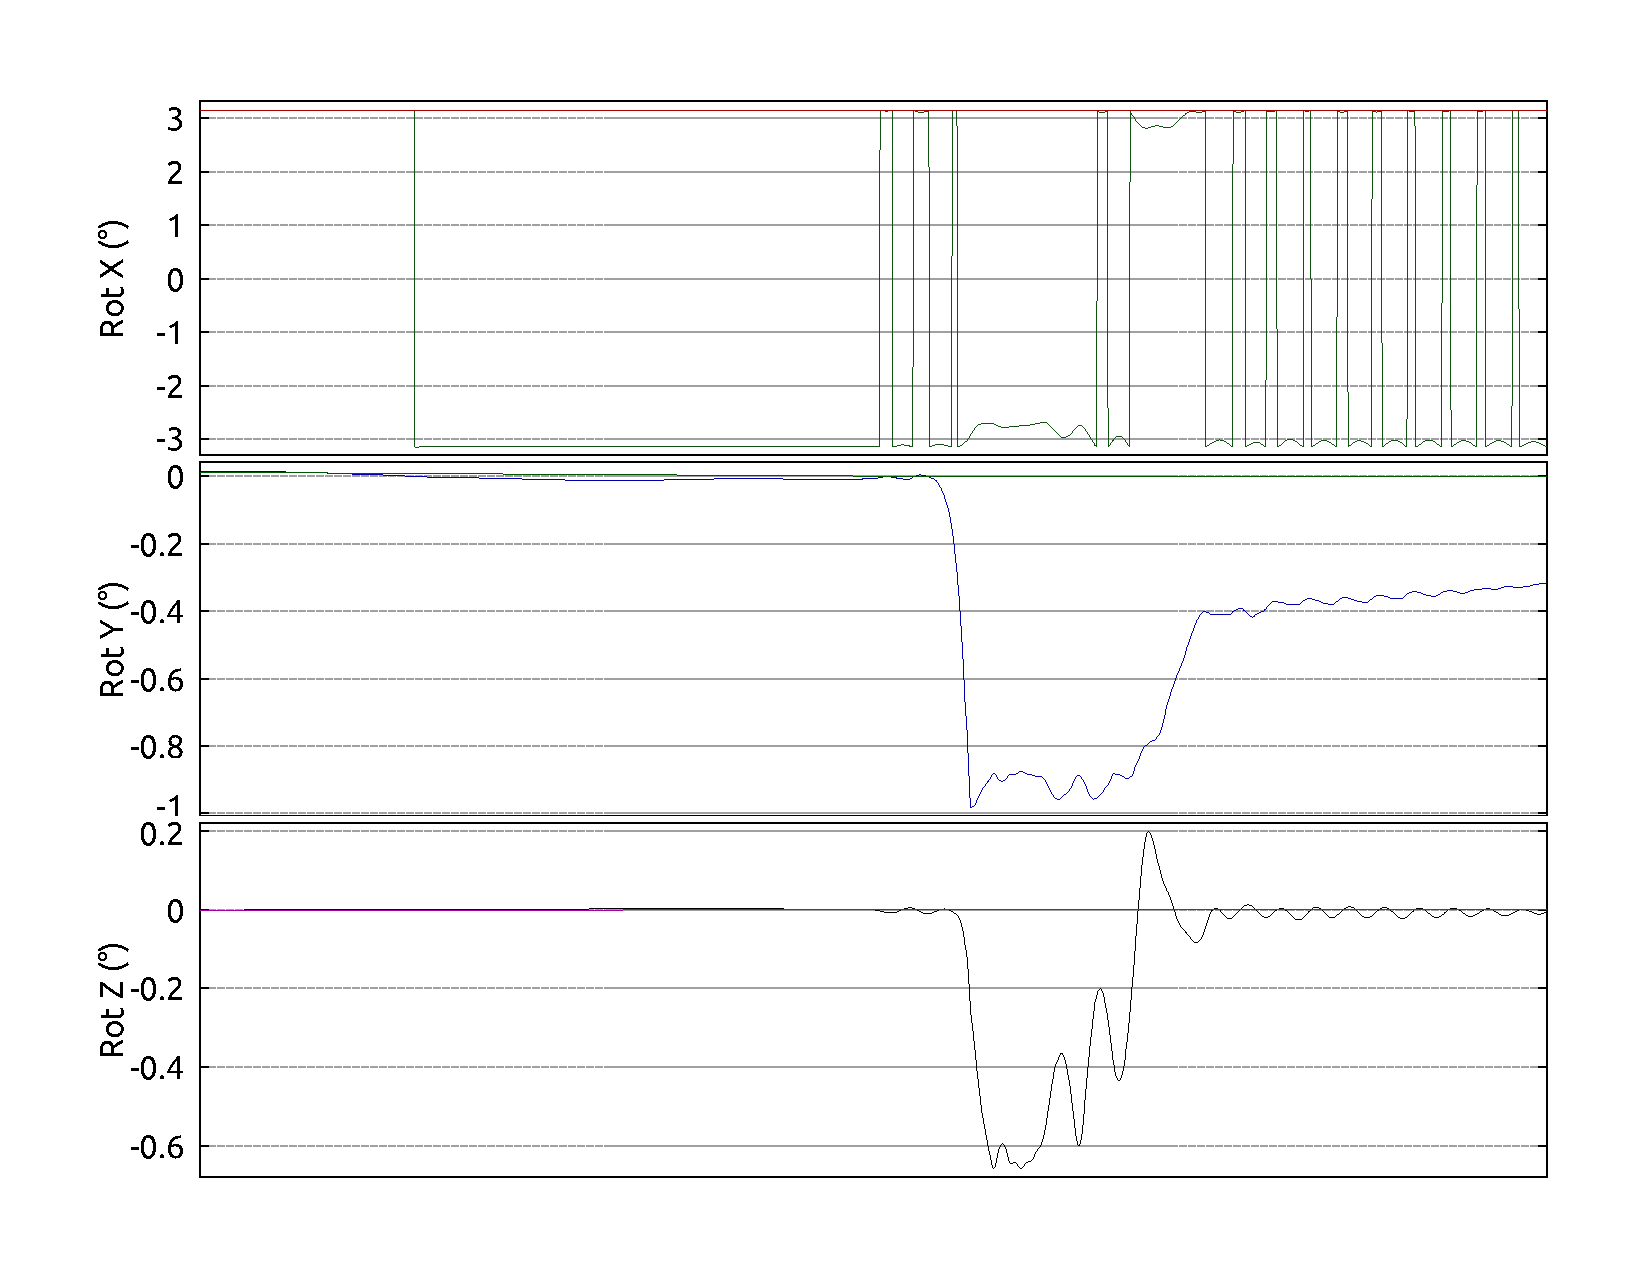
\includegraphics[width=\textwidth]{wound_1_zigzag_x_L5_20sec_orientation_track}
	\caption[Wound 2 printing trajectory tracking for ZigZag X path.]{Wound 2 printing trajectory tracking for ZigZag X path. (top) Position tracking. (bottom) Orientation tracking.}
    \label{fig:simulation_test_results_appendix_trajectory_tracking_wound_2_zizzag_x_tracking}
\end{figure}

\begin{figure}[htbp]
	\centering
	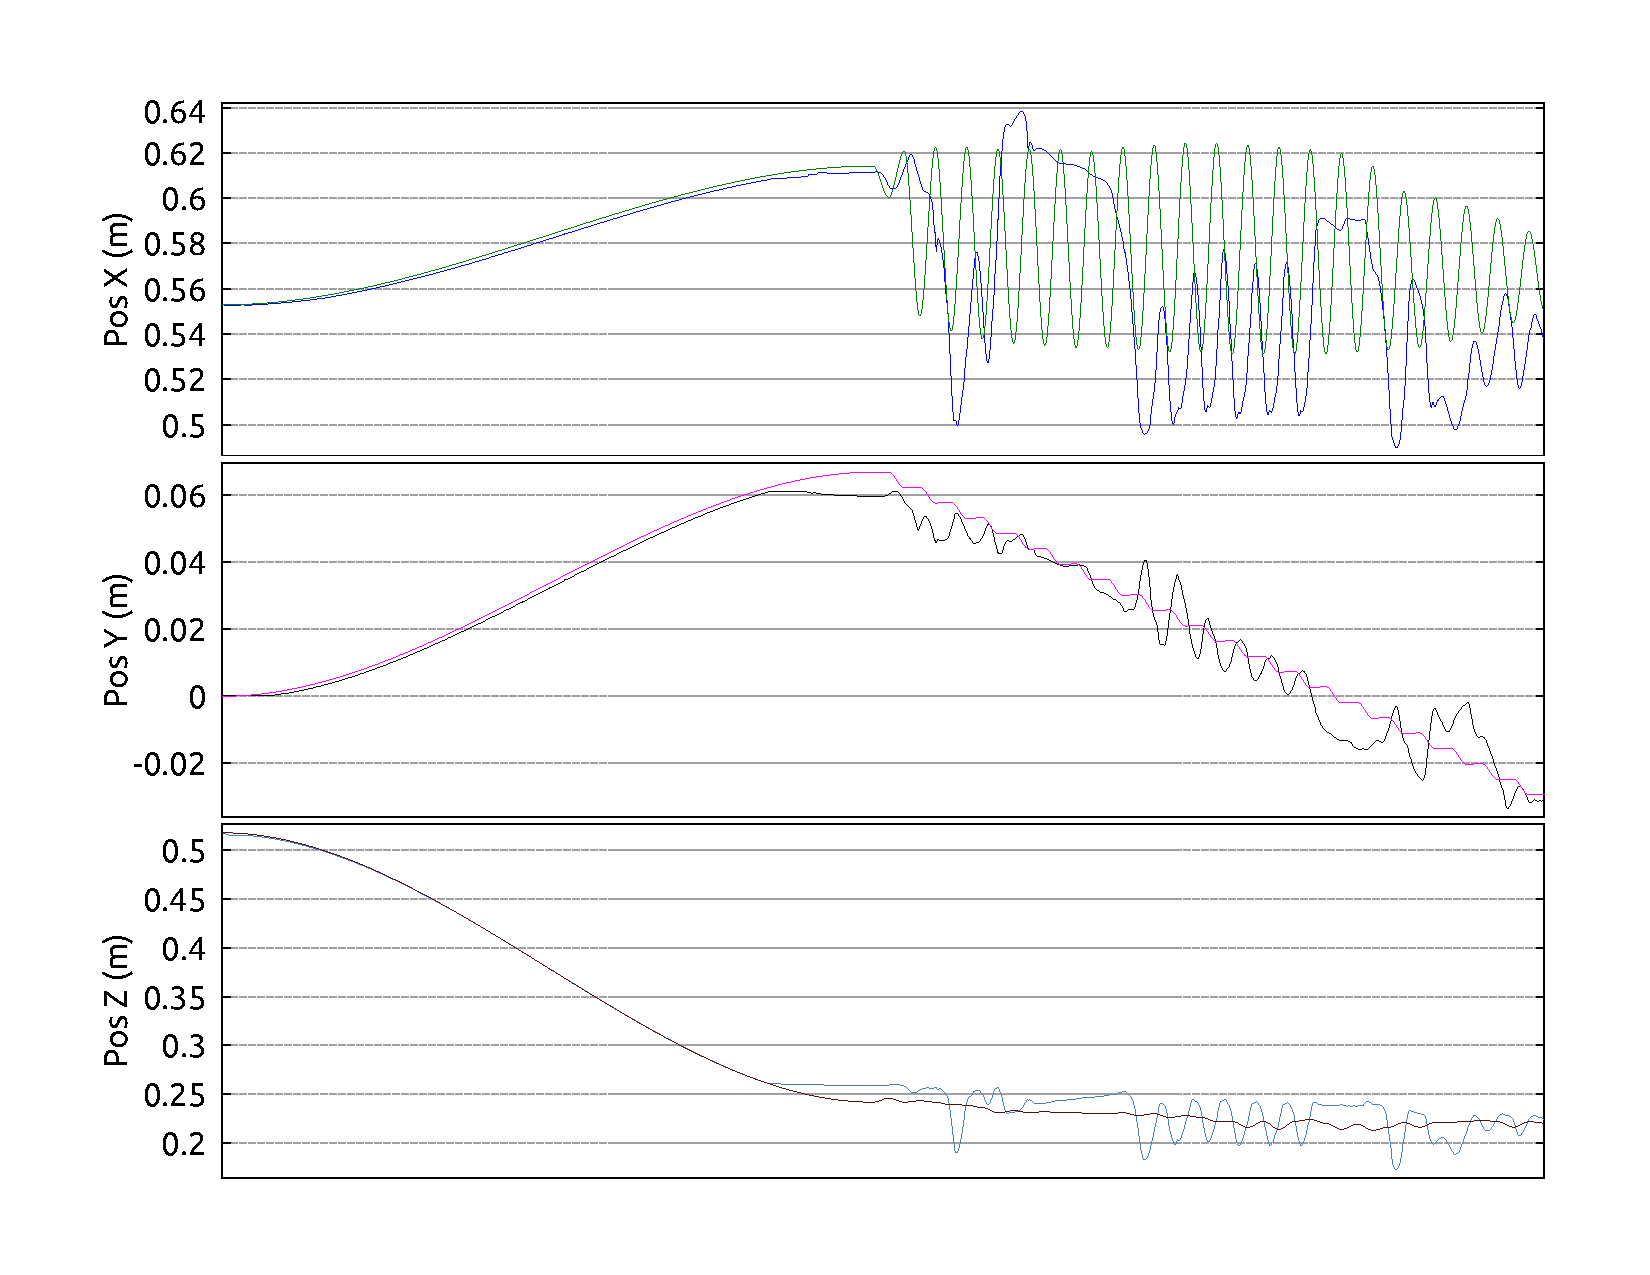
\includegraphics[width=\textwidth]{wound_1_zigzag_y_L5_20sec_position_track}
	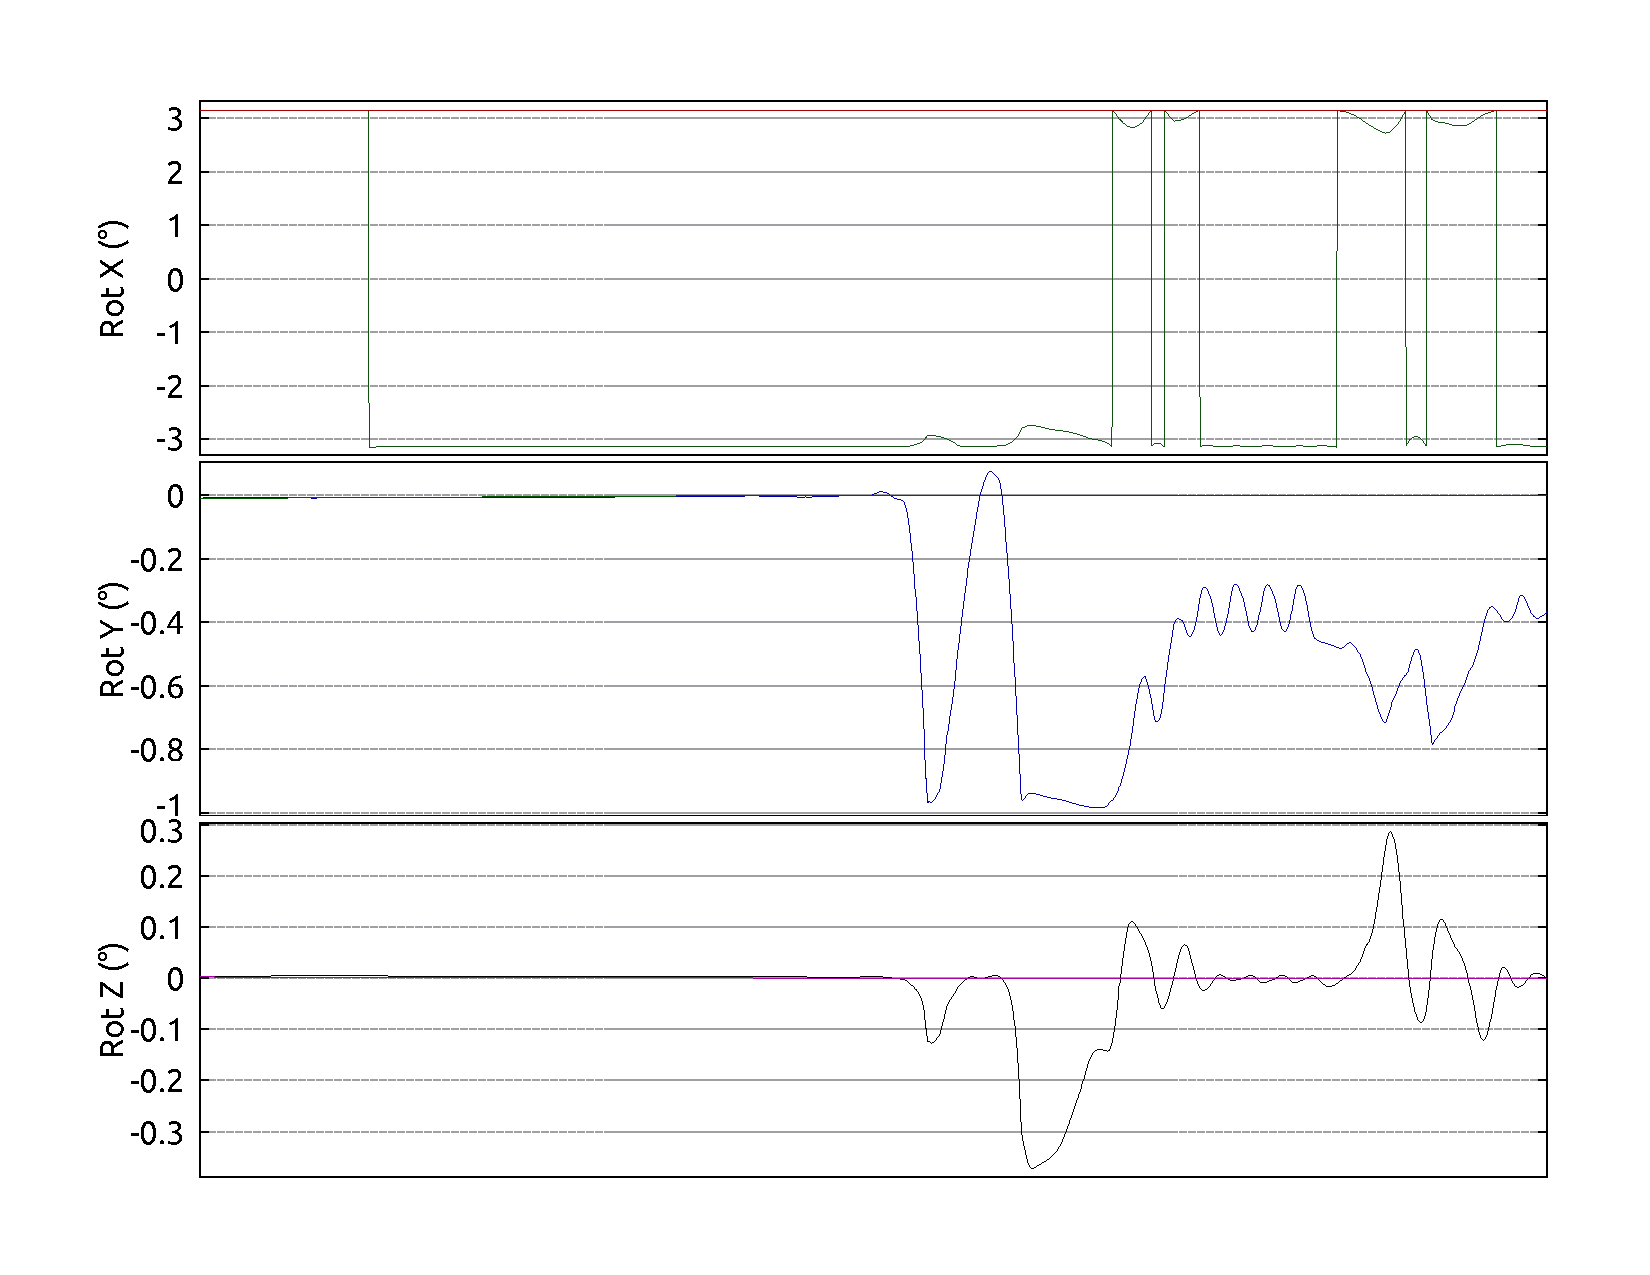
\includegraphics[width=\textwidth]{wound_1_zigzag_y_L5_20sec_orientation_track}
\caption[Wound 2 printing trajectory tracking for ZigZag Y path.]{Wound 2 printing trajectory tracking for ZigZag Y path. (top) Position tracking. (bottom) Orientation tracking.}
	\label{fig:simulation_test_results_appendix_trajectory_tracking_wound_2_zizzag_y_tracking}
\end{figure}

\begin{figure}[htbp]
	\centering
	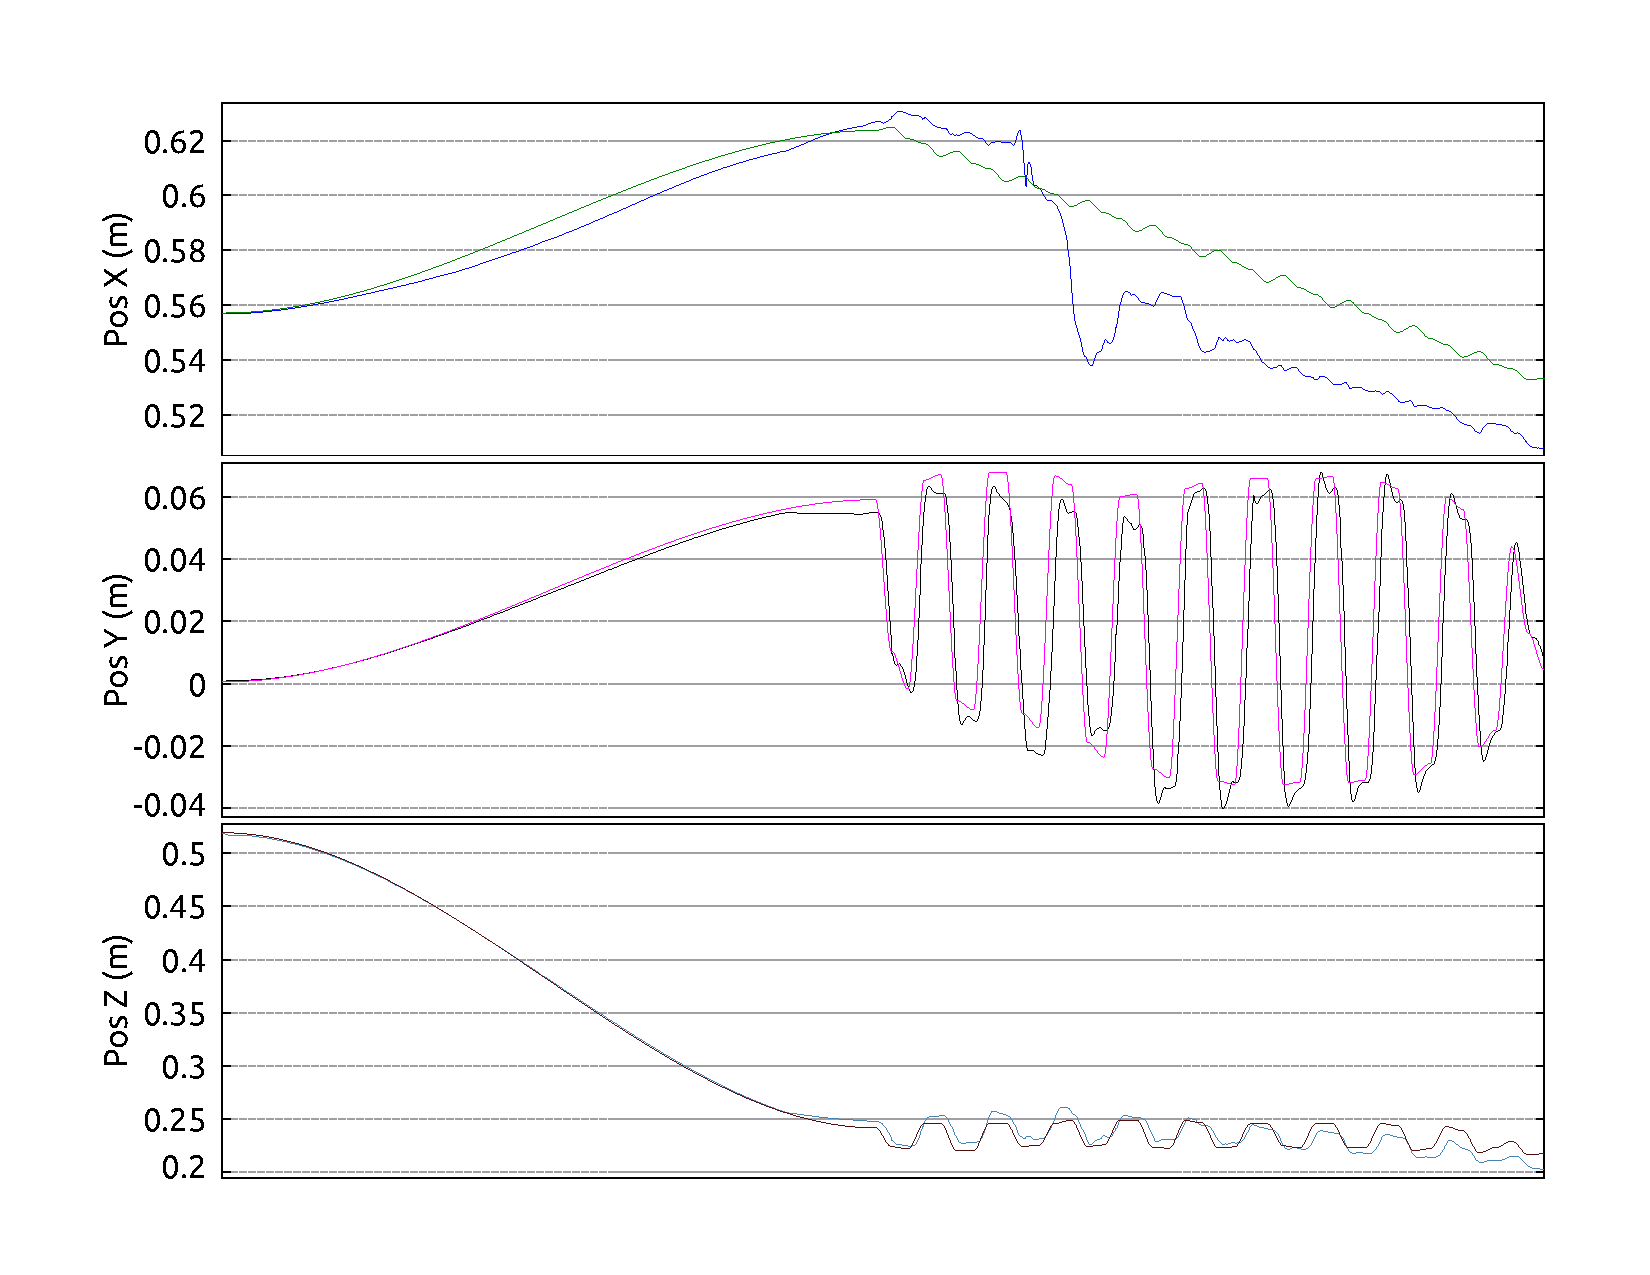
\includegraphics[width=\textwidth]{wound_1_parallel_x_L5_20sec_position_track}
	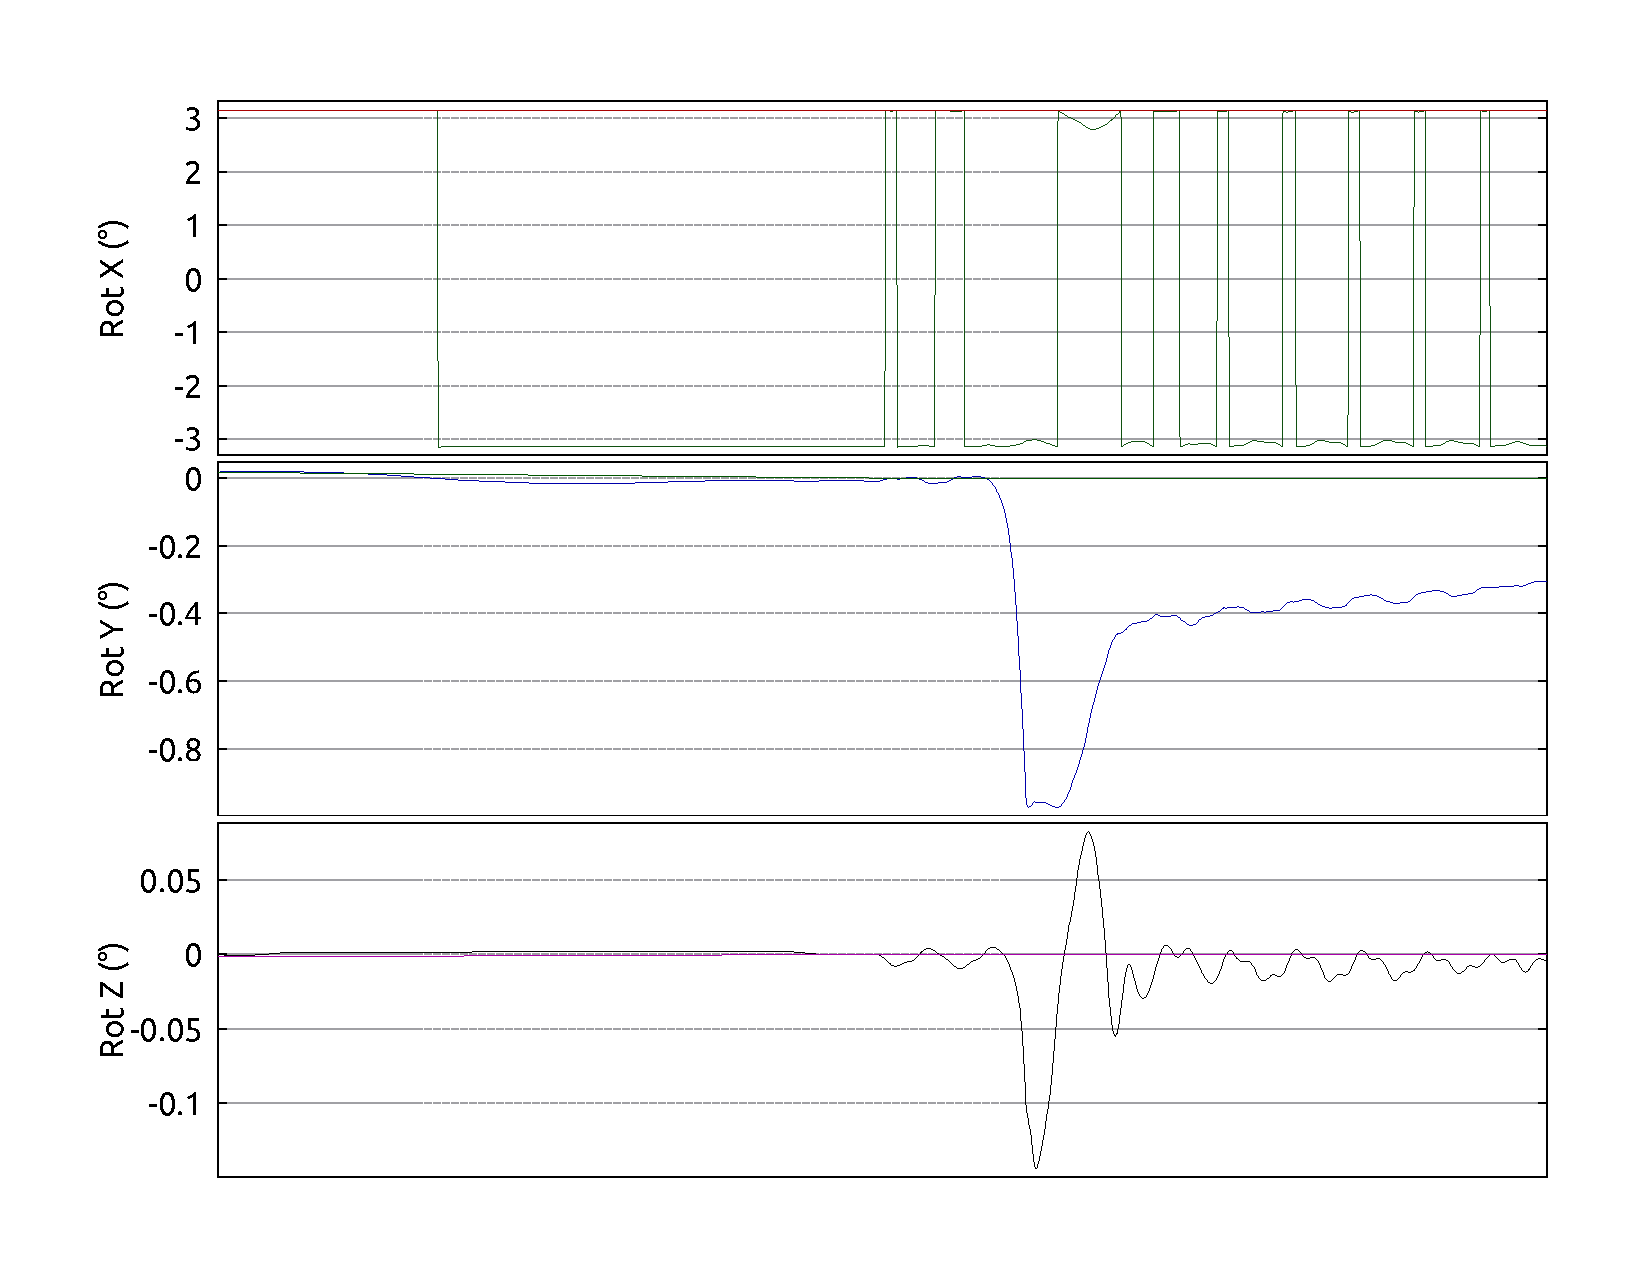
\includegraphics[width=\textwidth]{wound_1_parallel_x_L5_20sec_orientation_track}
	\caption[Wound 2 printing trajectory tracking for Parallel Lines X path.]{Wound 2 printing trajectory tracking for Parallel Lines X path. (top) Position tracking. (bottom) Orientation tracking.}
	\label{fig:simulation_test_results_appendix_trajectory_tracking_wound_2_parallel_x_tracking}
\end{figure}

\begin{figure}[htbp]
	\centering
	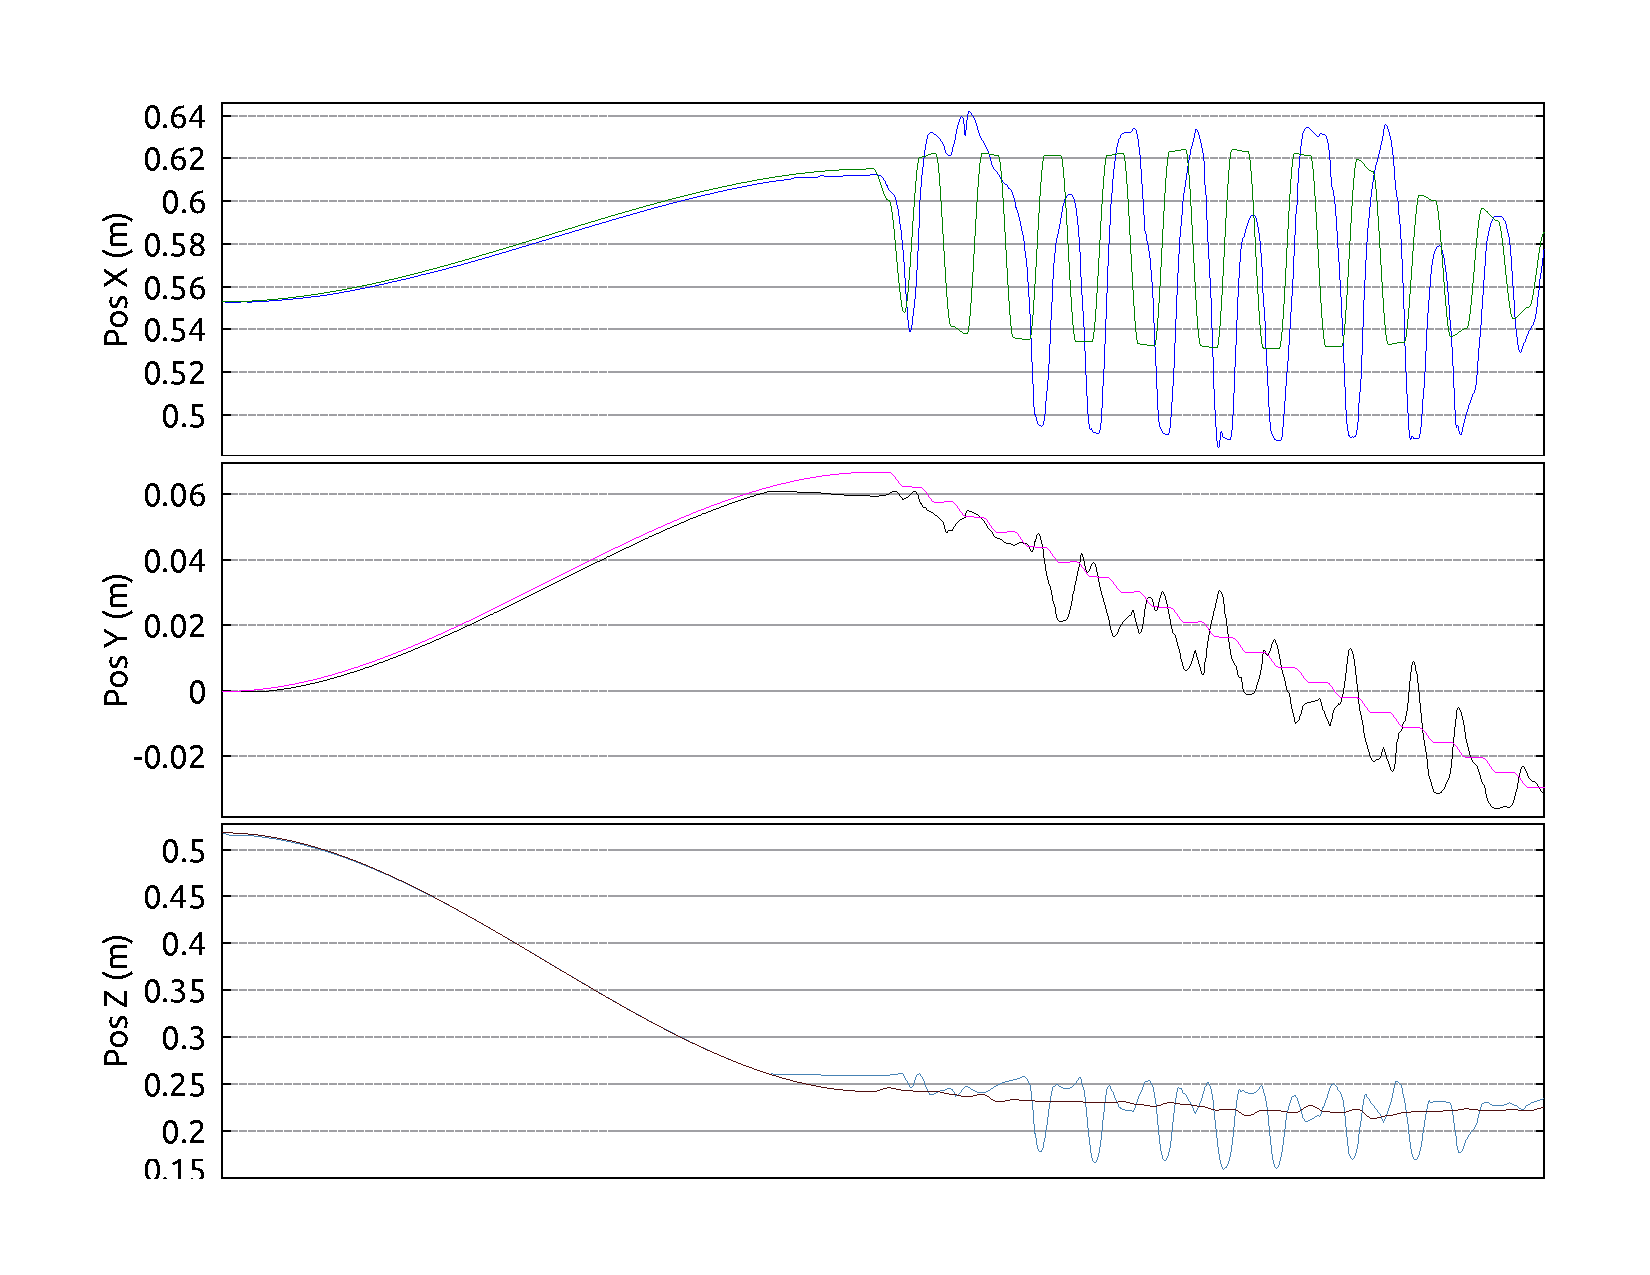
\includegraphics[width=\textwidth]{wound_1_parallel_y_L5_20sec_position_track}
	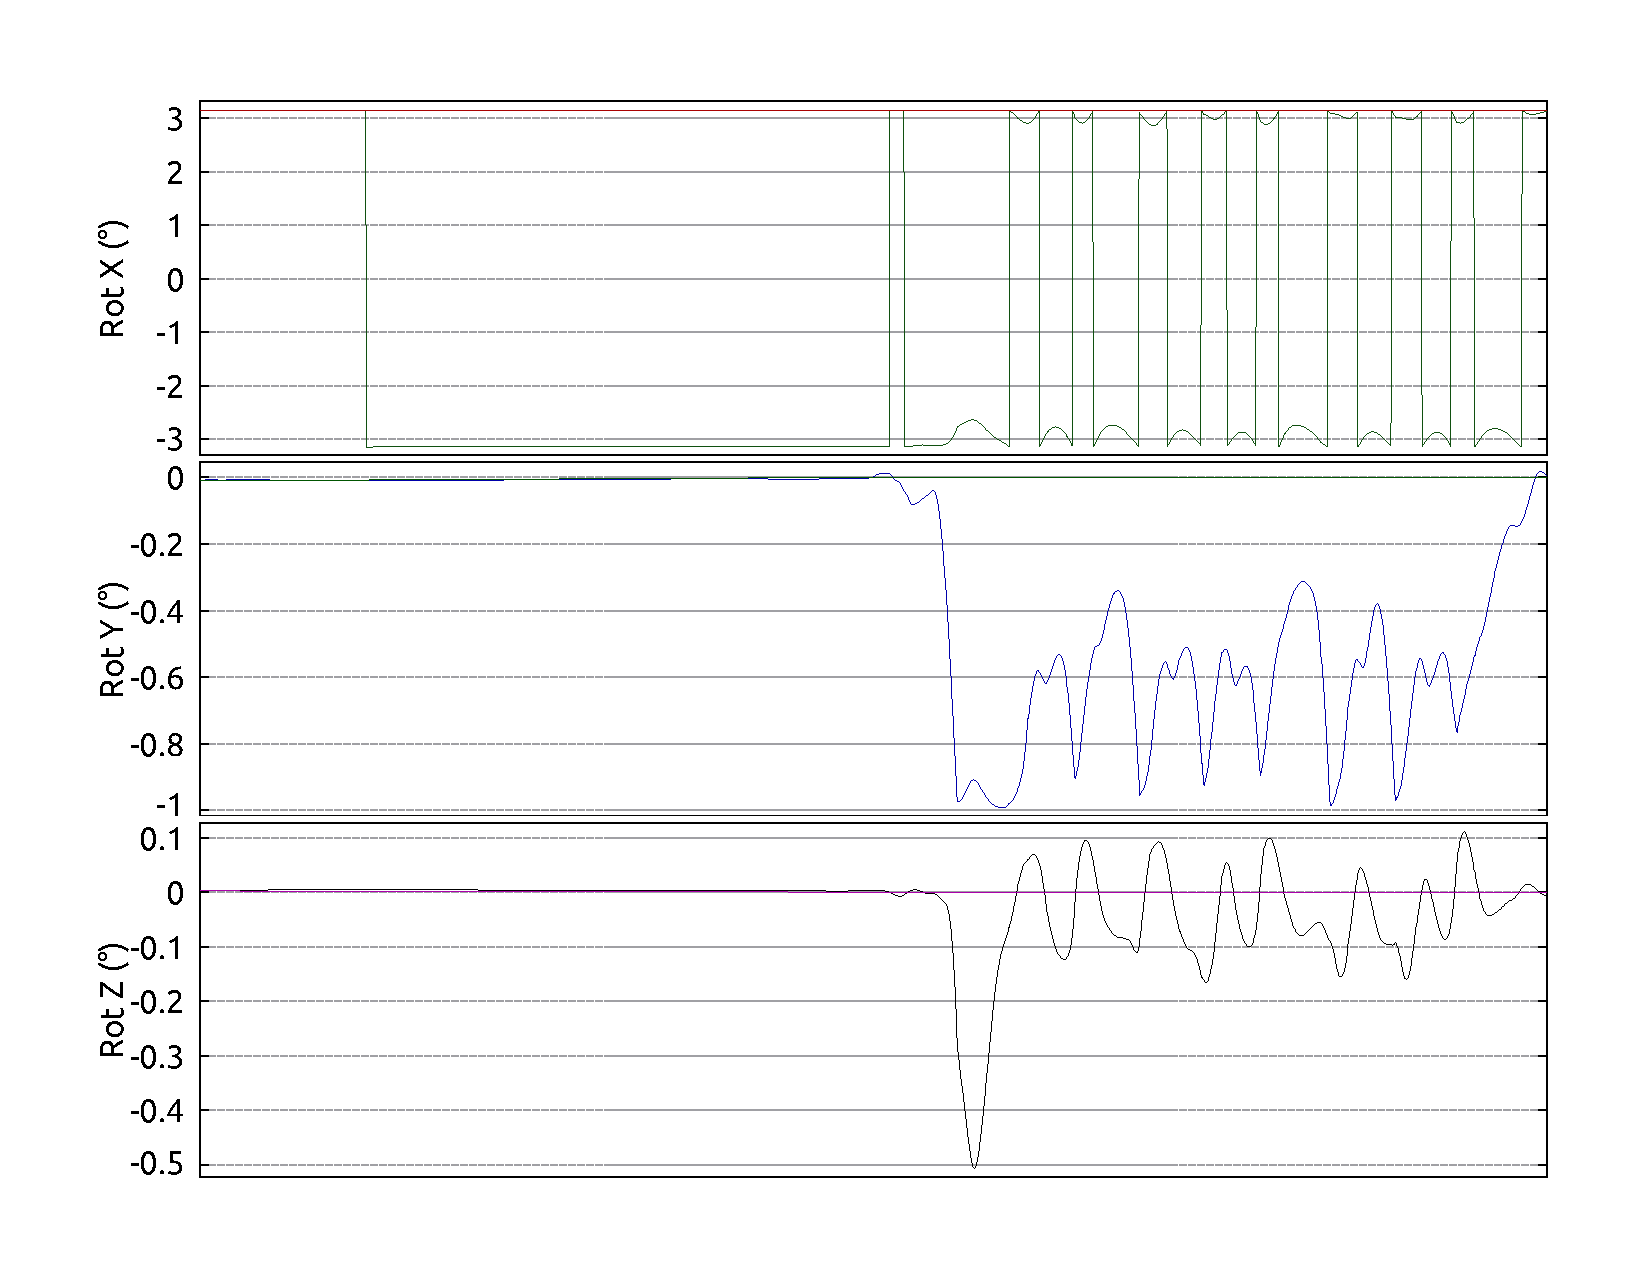
\includegraphics[width=\textwidth]{wound_1_parallel_y_L5_20sec_orientation_track}
    \caption[Wound 2 printing trajectory tracking for Parallel Lines Y path.]{Wound 2 printing trajectory tracking for Parallel Lines Y path. (top) Position tracking. (bottom) Orientation tracking.}
	\label{fig:simulation_test_results_appendix_trajectory_tracking_wound_2_parallel_y_tracking}
\end{figure}

\begin{figure}[htbp]
	\centering
	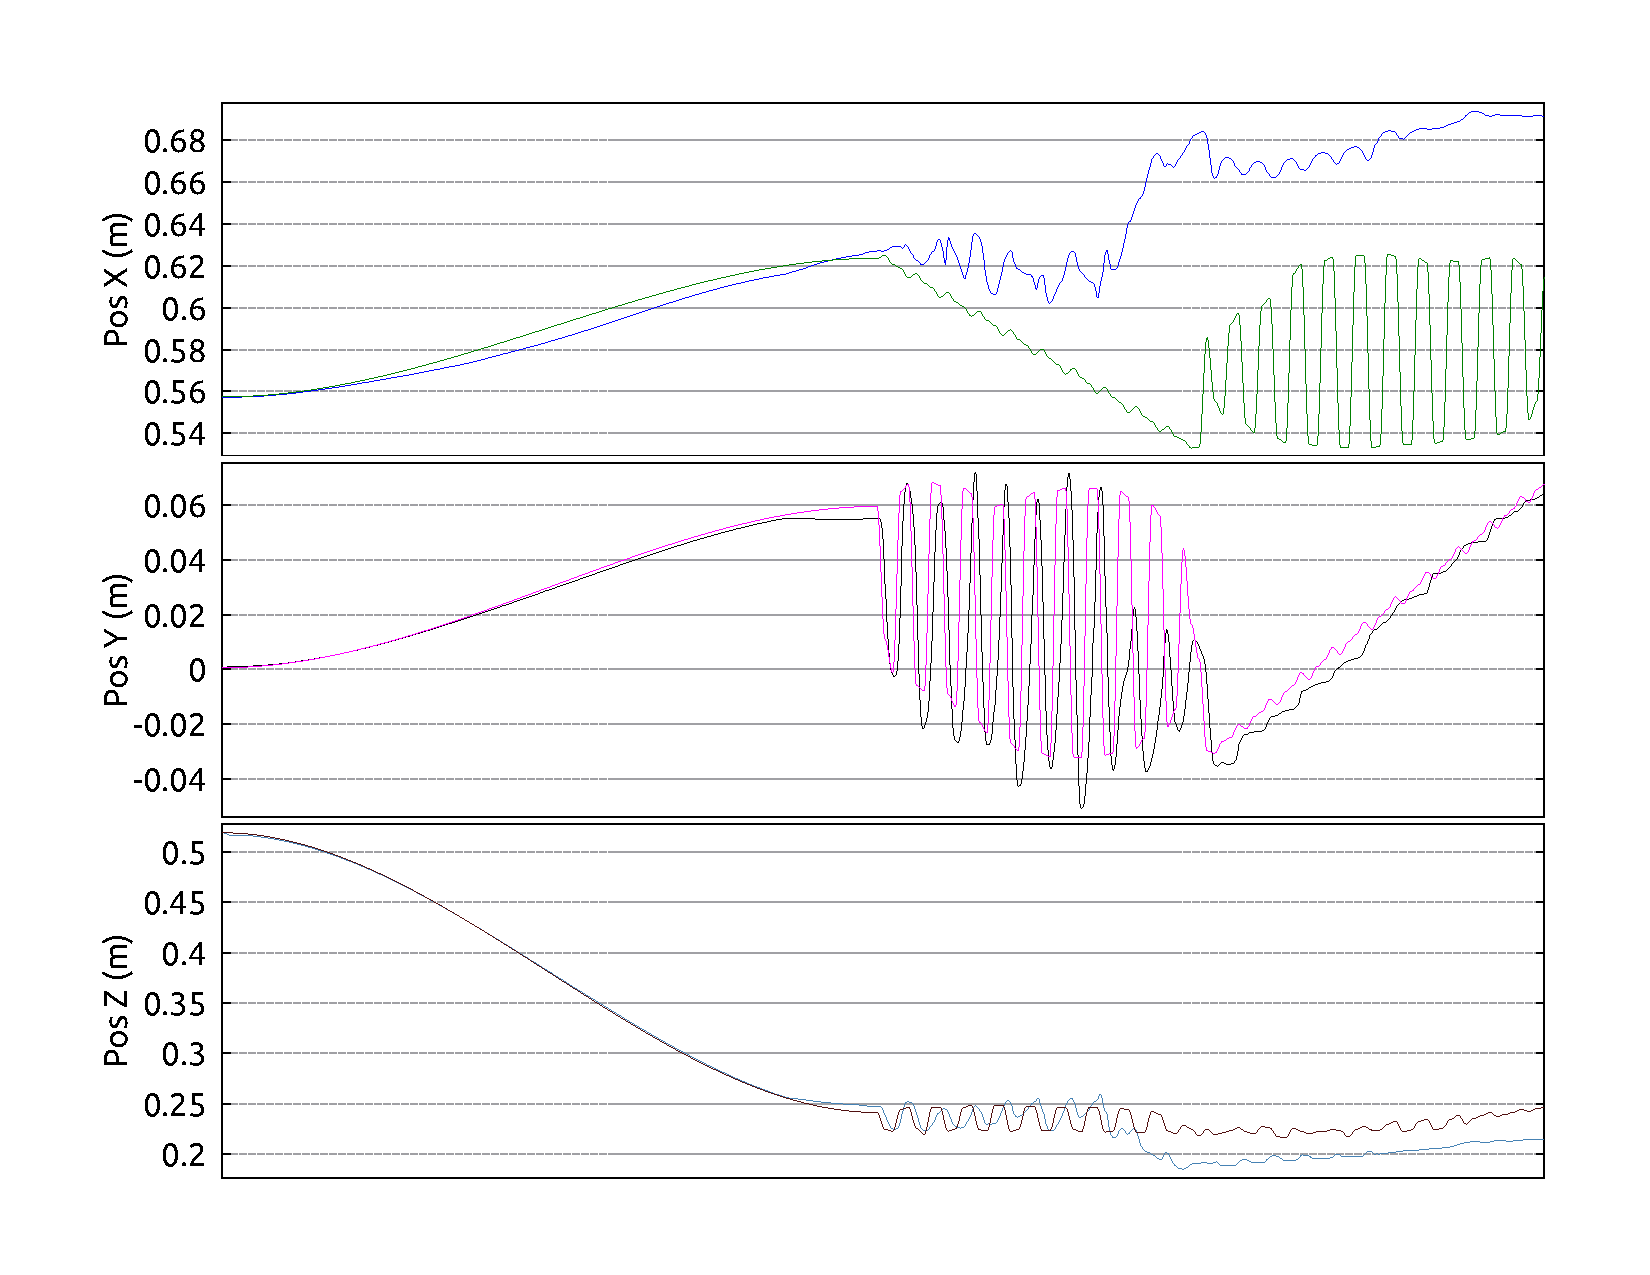
\includegraphics[width=\textwidth]{wound_1_grid_L5_20sec_position_track}
	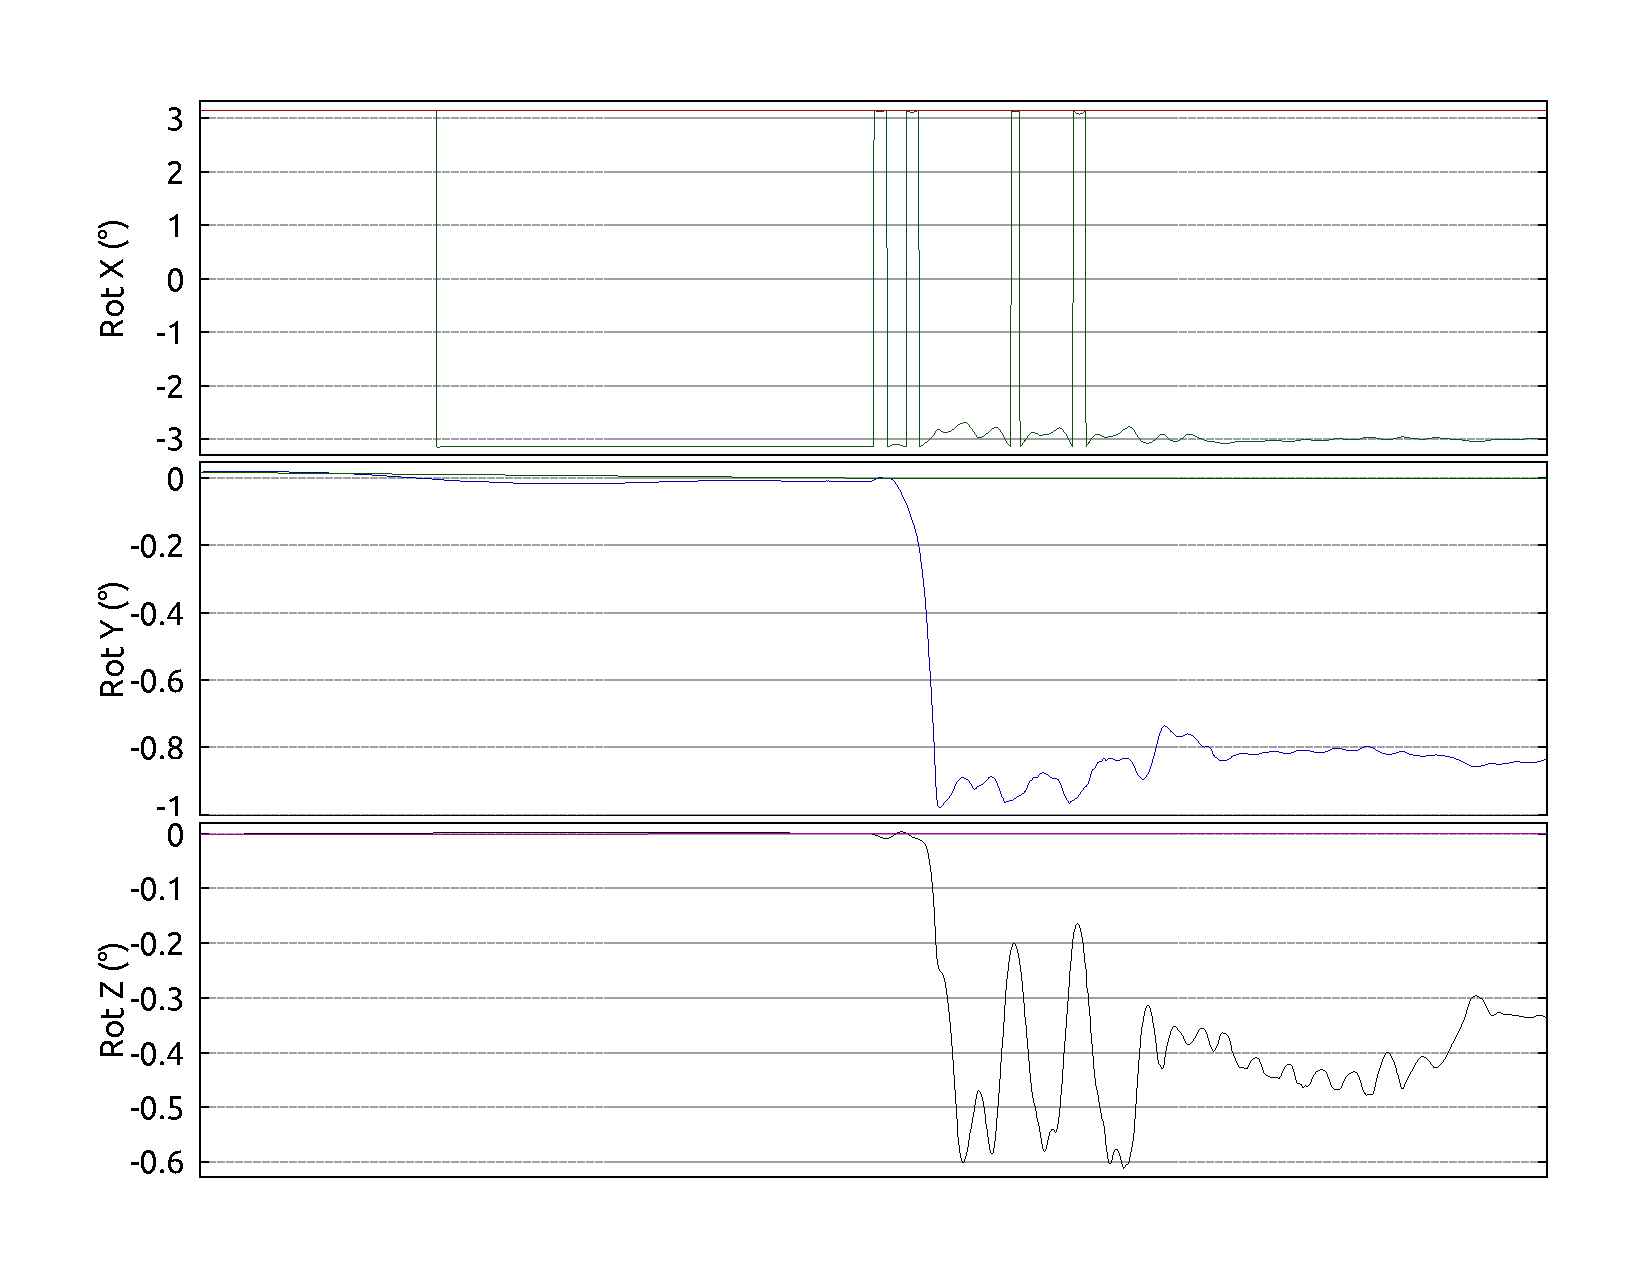
\includegraphics[width=\textwidth]{wound_1_grid_L5_20sec_orientation_track}
    \caption[Wound 2 printing trajectory tracking for Grid path.]{Wound 2 printing trajectory tracking for Grid path. (top) Position tracking. (bottom) Orientation tracking.}
	\label{fig:simulation_test_results_appendix_trajectory_tracking_wound_2_grid_tracking}
\end{figure}

% ------------------------
% Wound 3
% ------------------------

\begin{figure}[htbp]
	\centering
	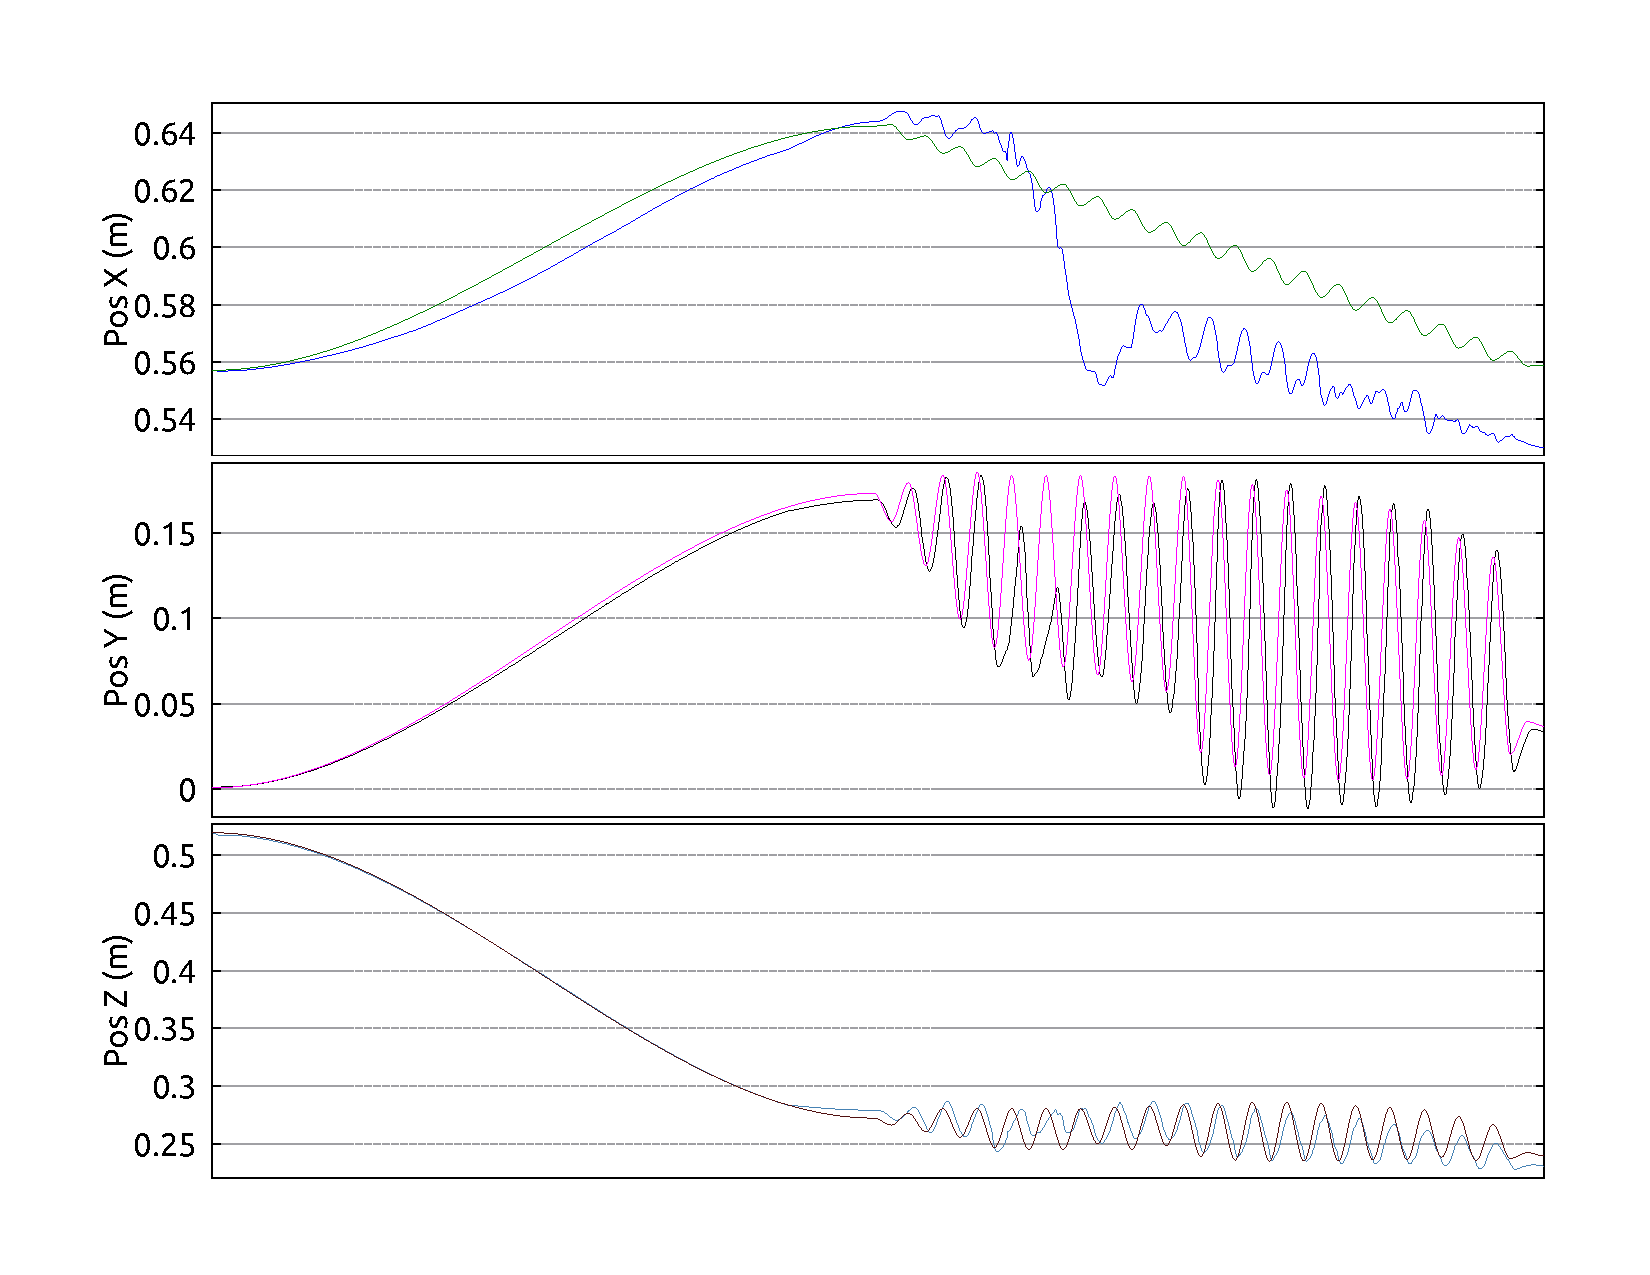
\includegraphics[width=\textwidth]{wound_2_zigzag_x_L5_20sec_position_track}
	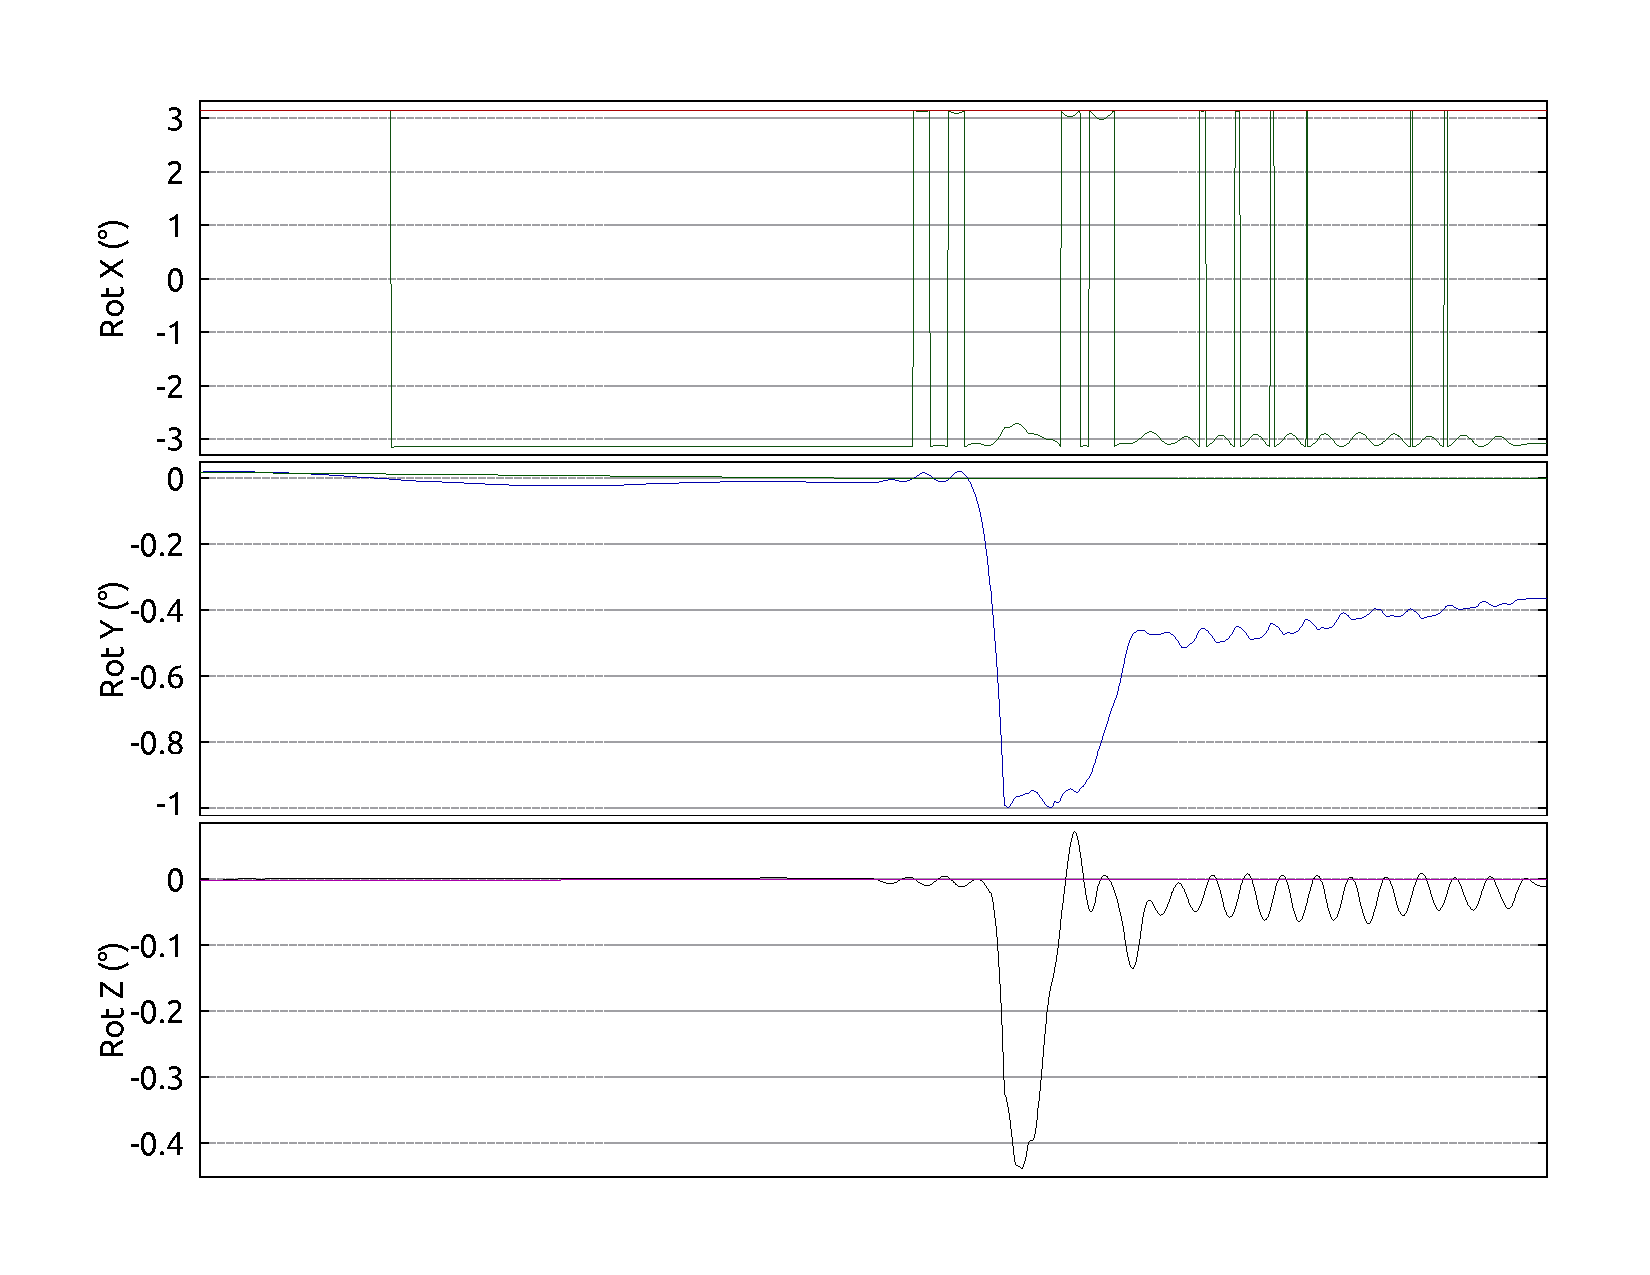
\includegraphics[width=\textwidth]{wound_2_zigzag_x_L5_20sec_orientation_track}
	\caption[Wound 3 printing trajectory tracking for ZigZag X path.]{Wound 3 printing trajectory tracking for ZigZag X path. (top) Position tracking. (bottom) Orientation tracking.}
    \label{fig:simulation_test_results_appendix_trajectory_tracking_wound_3_zizzag_x_tracking}
\end{figure}

\begin{figure}[htbp]
	\centering
	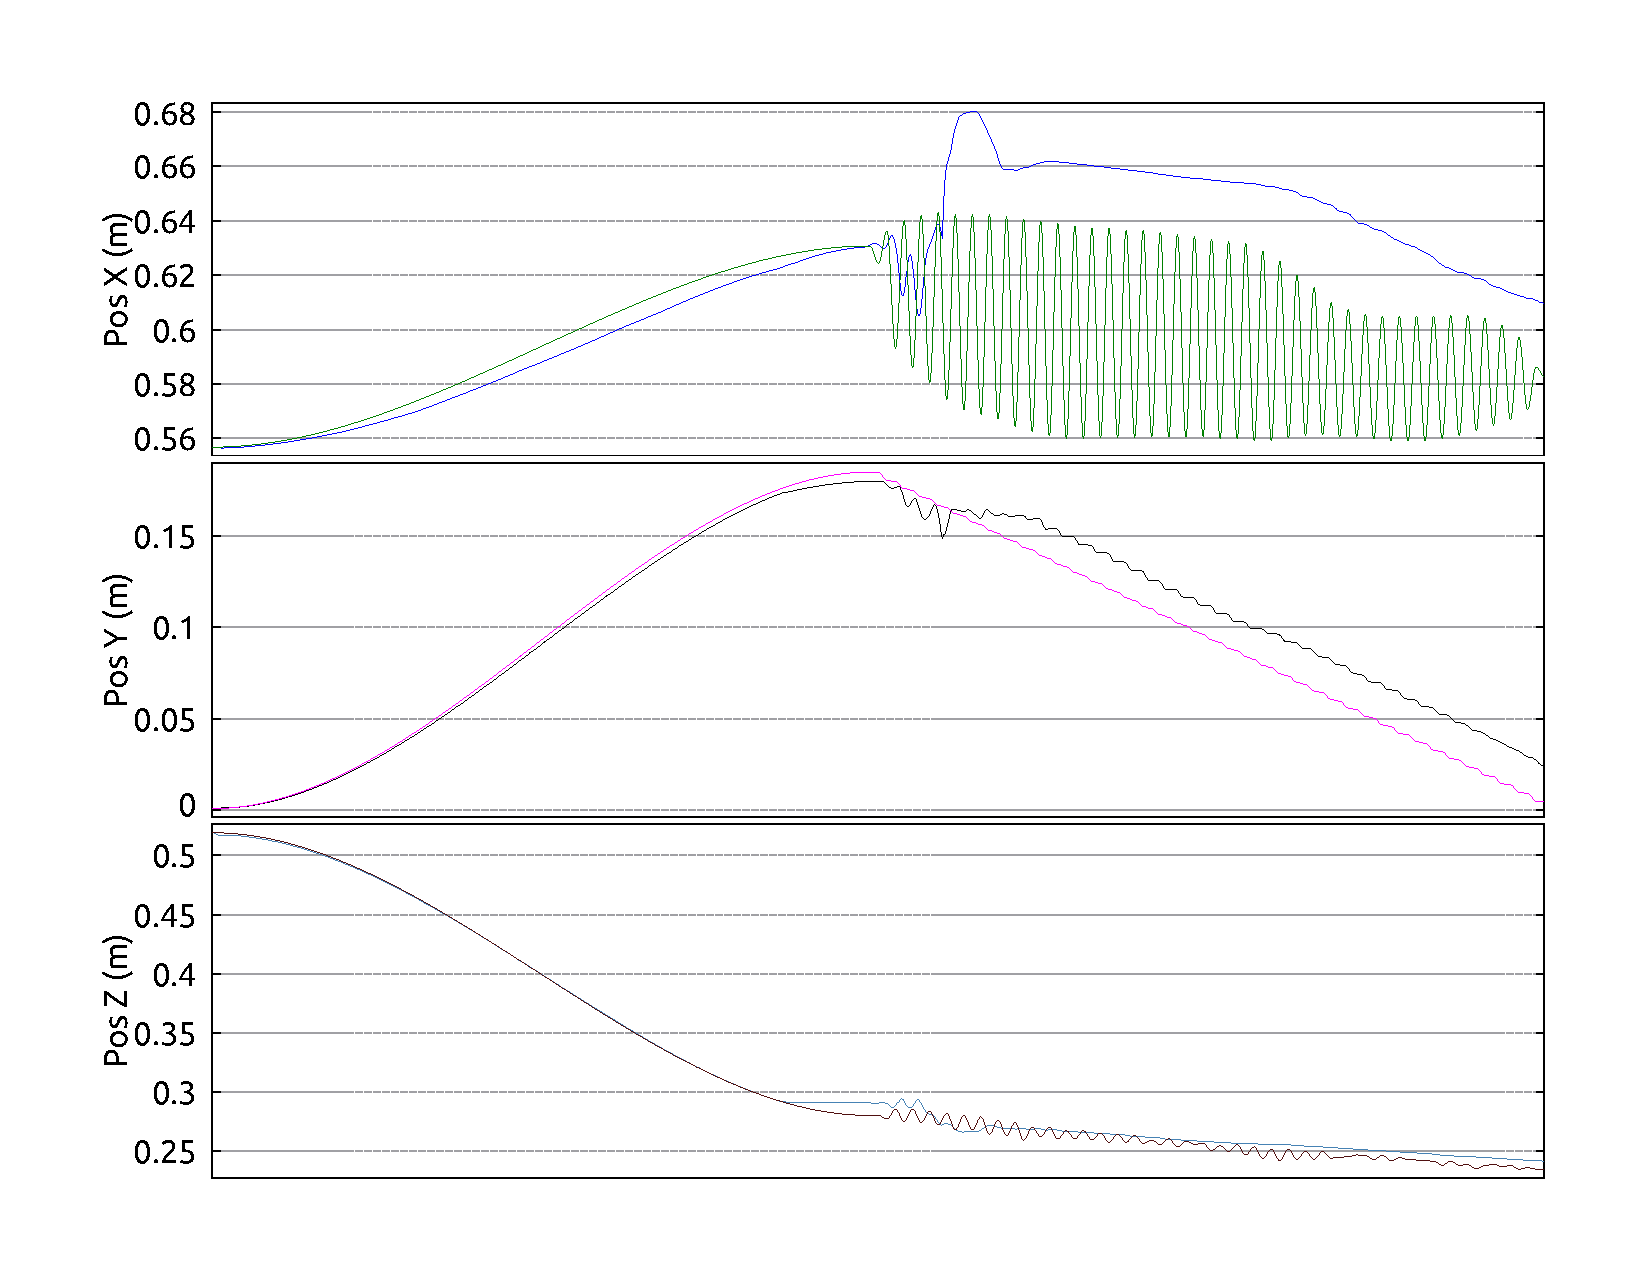
\includegraphics[width=\textwidth]{wound_2_zigzag_y_L5_20sec_position_track}
	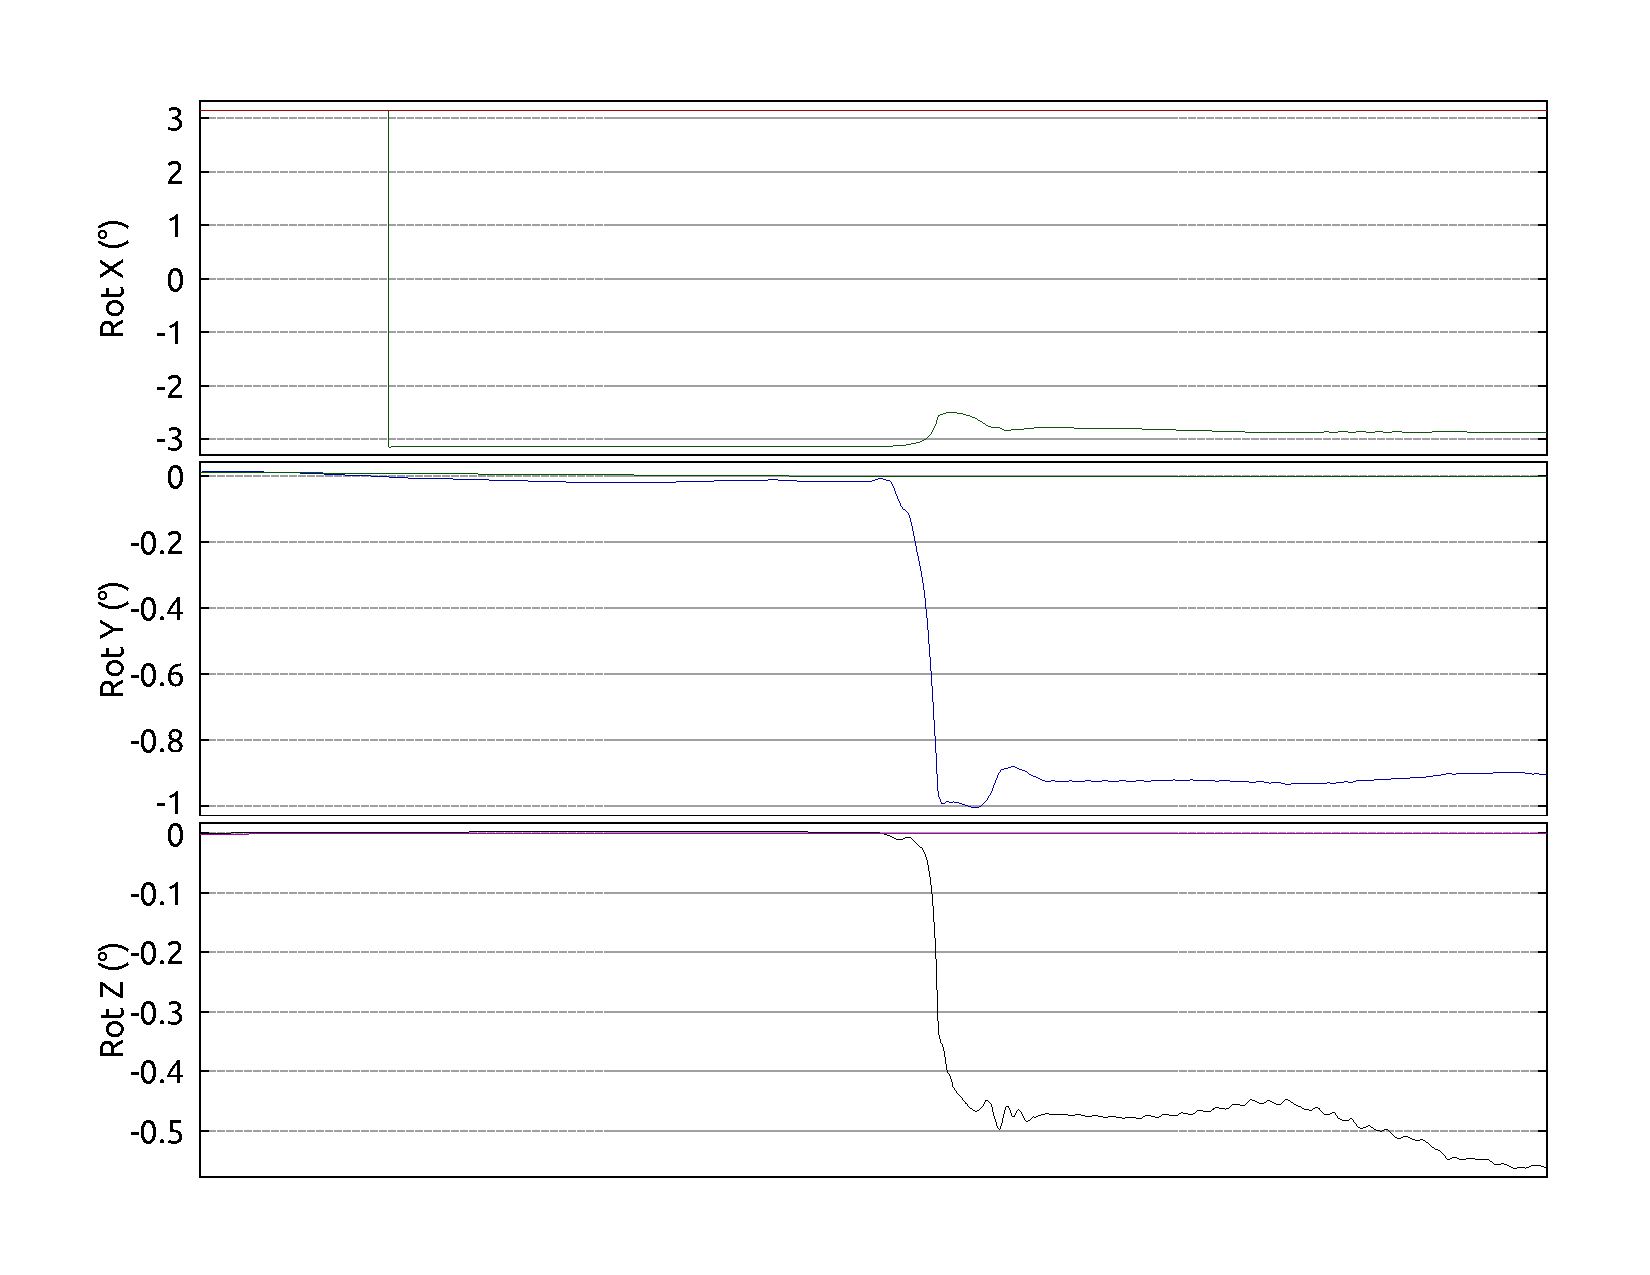
\includegraphics[width=\textwidth]{wound_2_zigzag_y_L5_20sec_orientation_track}
\caption[Wound 3 printing trajectory tracking for ZigZag Y path.]{Wound 3 printing trajectory tracking for ZigZag Y path. (top) Position tracking. (bottom) Orientation tracking.}
	\label{fig:simulation_test_results_appendix_trajectory_tracking_wound_3_zizzag_y_tracking}
\end{figure}

\begin{figure}[htbp]
	\centering
	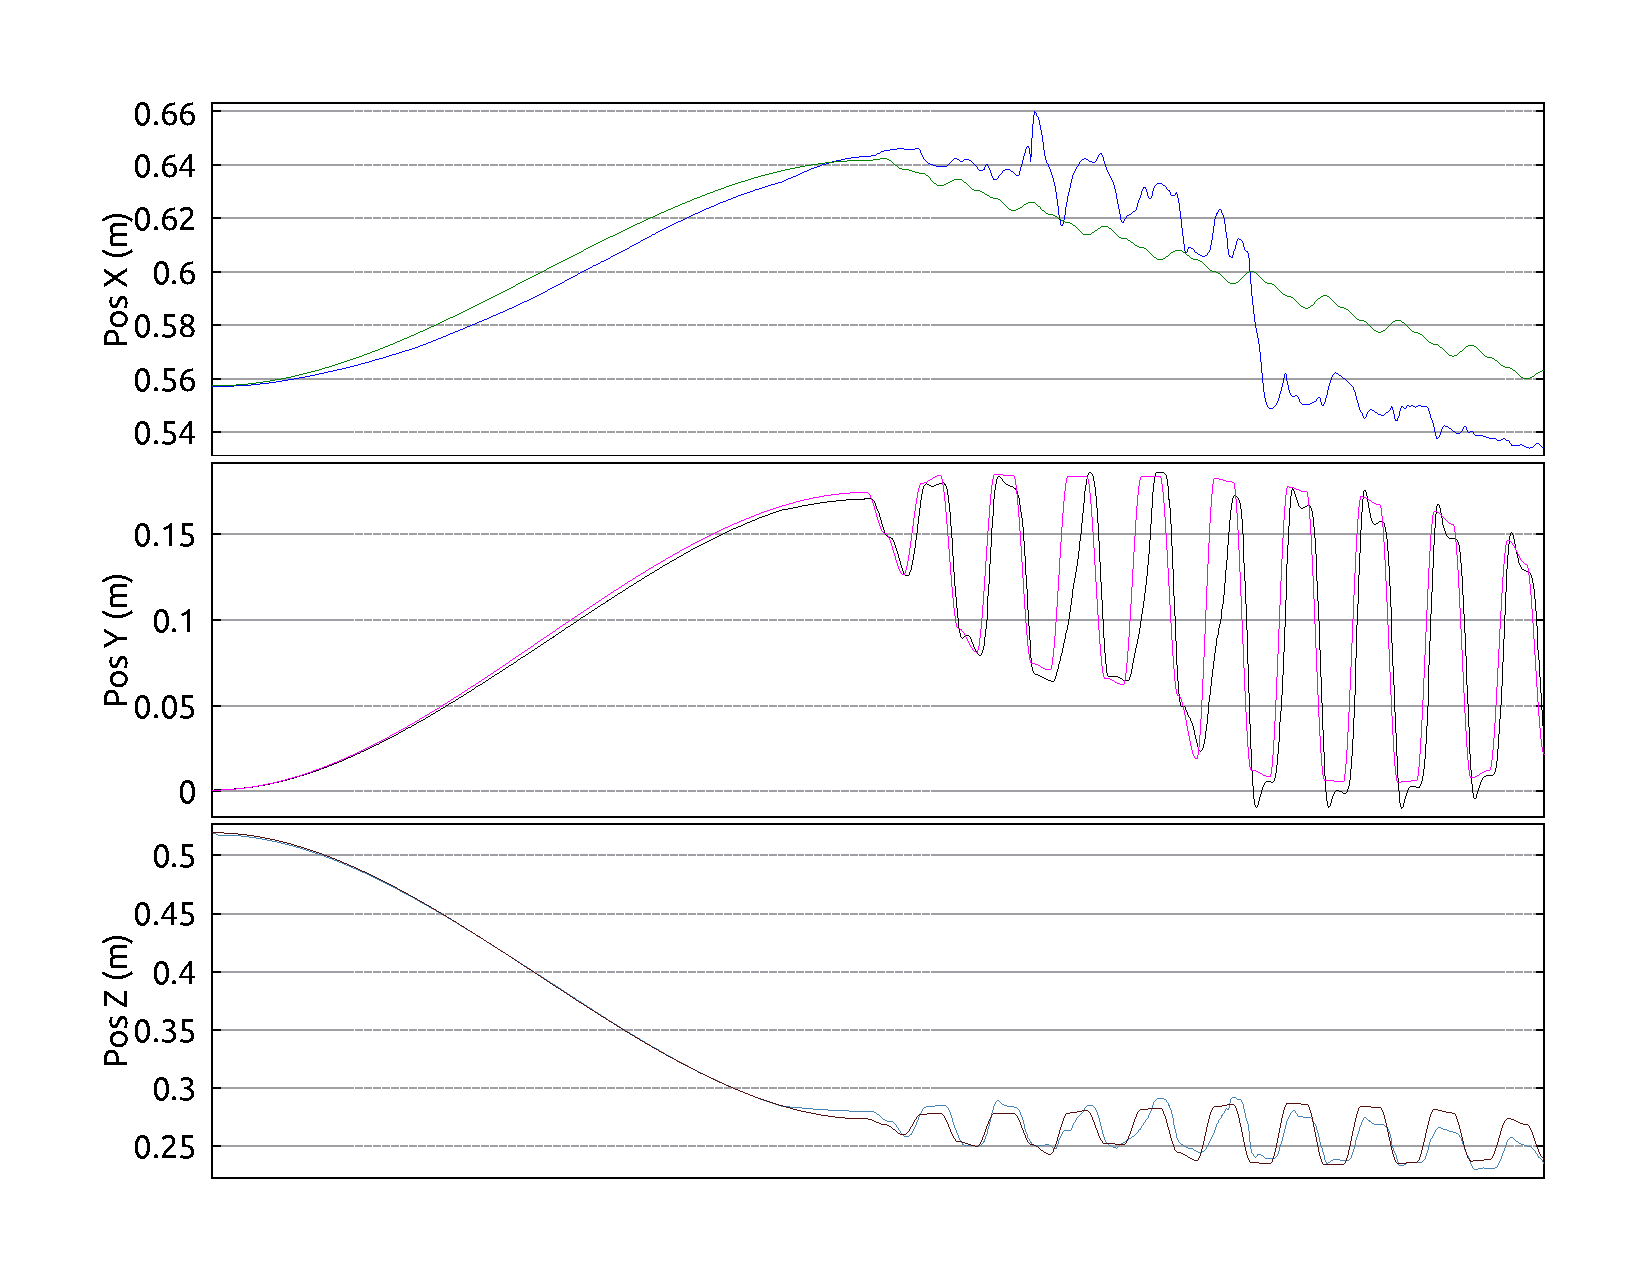
\includegraphics[width=\textwidth]{wound_2_parallel_x_L5_20sec_position_track}
	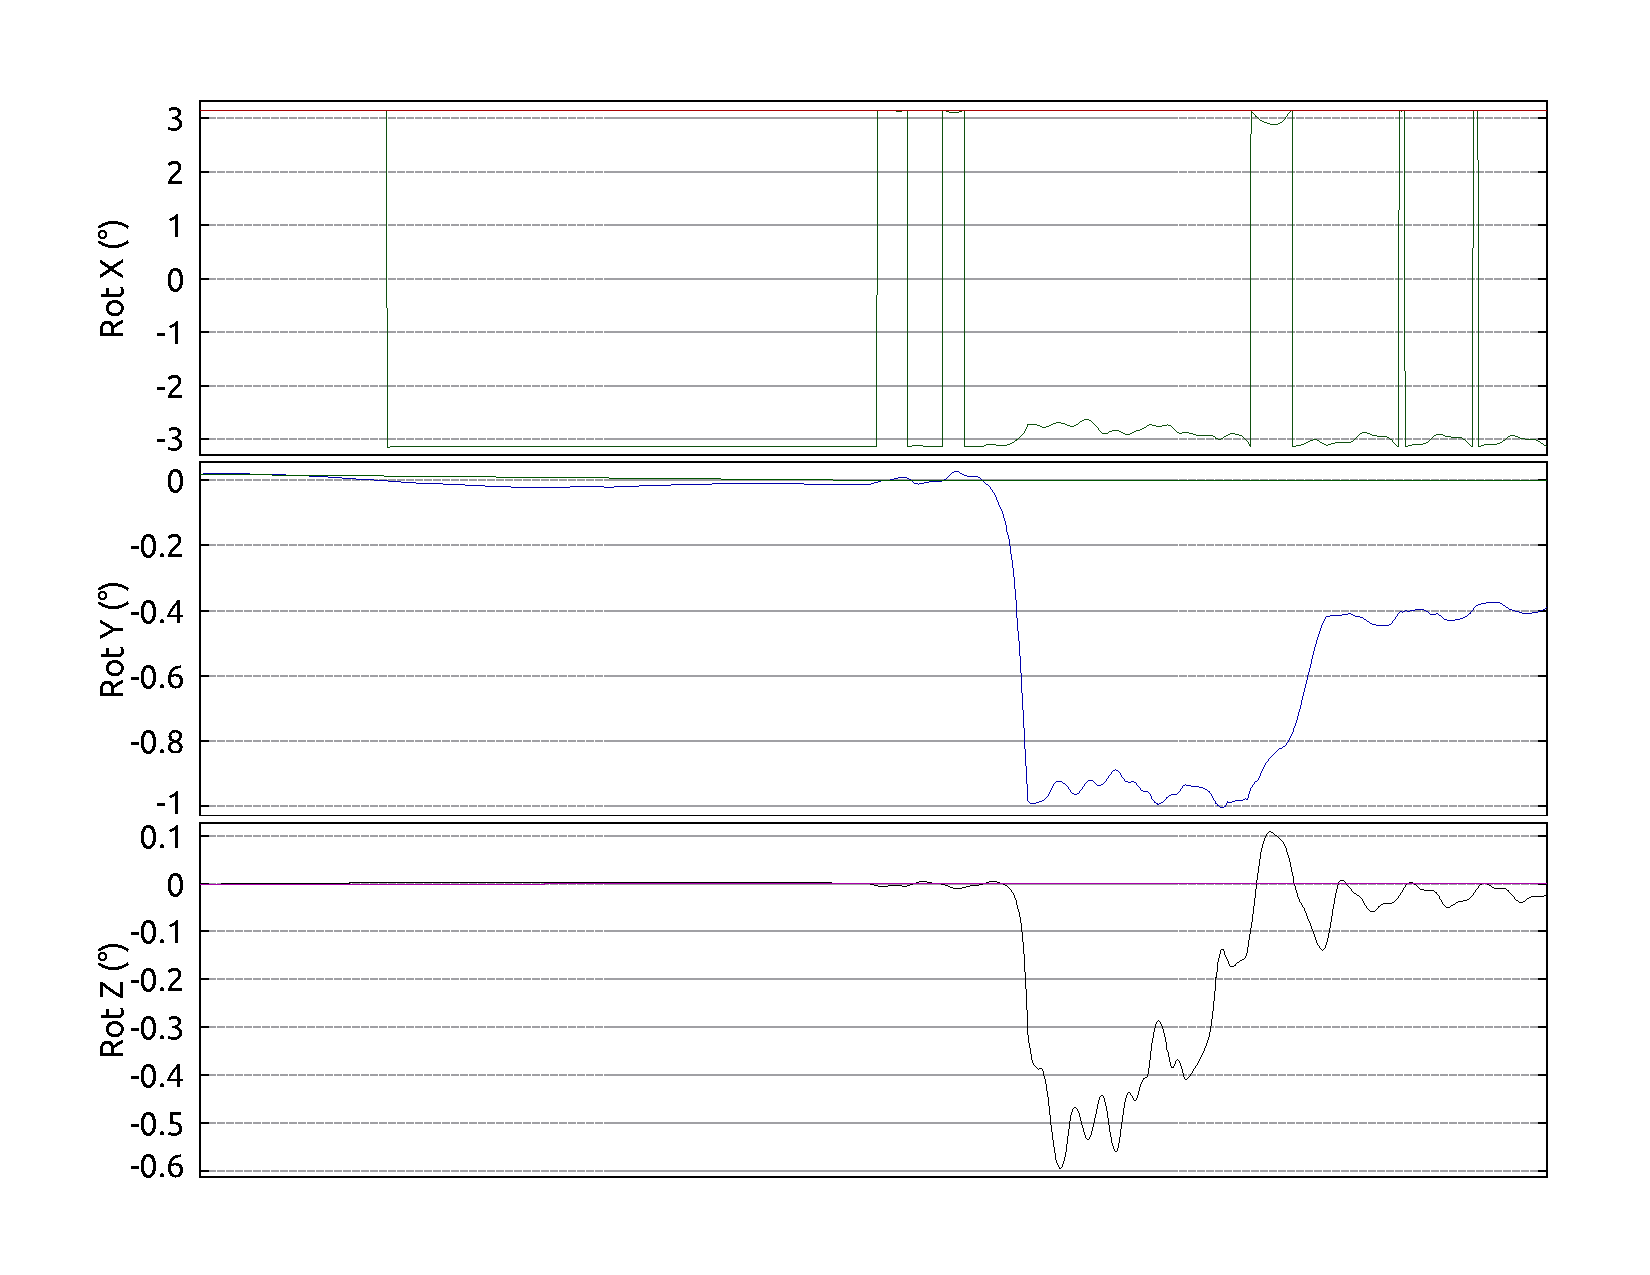
\includegraphics[width=\textwidth]{wound_2_parallel_x_L5_20sec_orientation_track}
	\caption[Wound 3 printing trajectory tracking for Parallel Lines X path.]{Wound 3 printing trajectory tracking for Parallel Lines X path. (top) Position tracking. (bottom) Orientation tracking.}
	\label{fig:simulation_test_results_appendix_trajectory_tracking_wound_3_parallel_x_tracking}
\end{figure}

\begin{figure}[htbp]
	\centering
	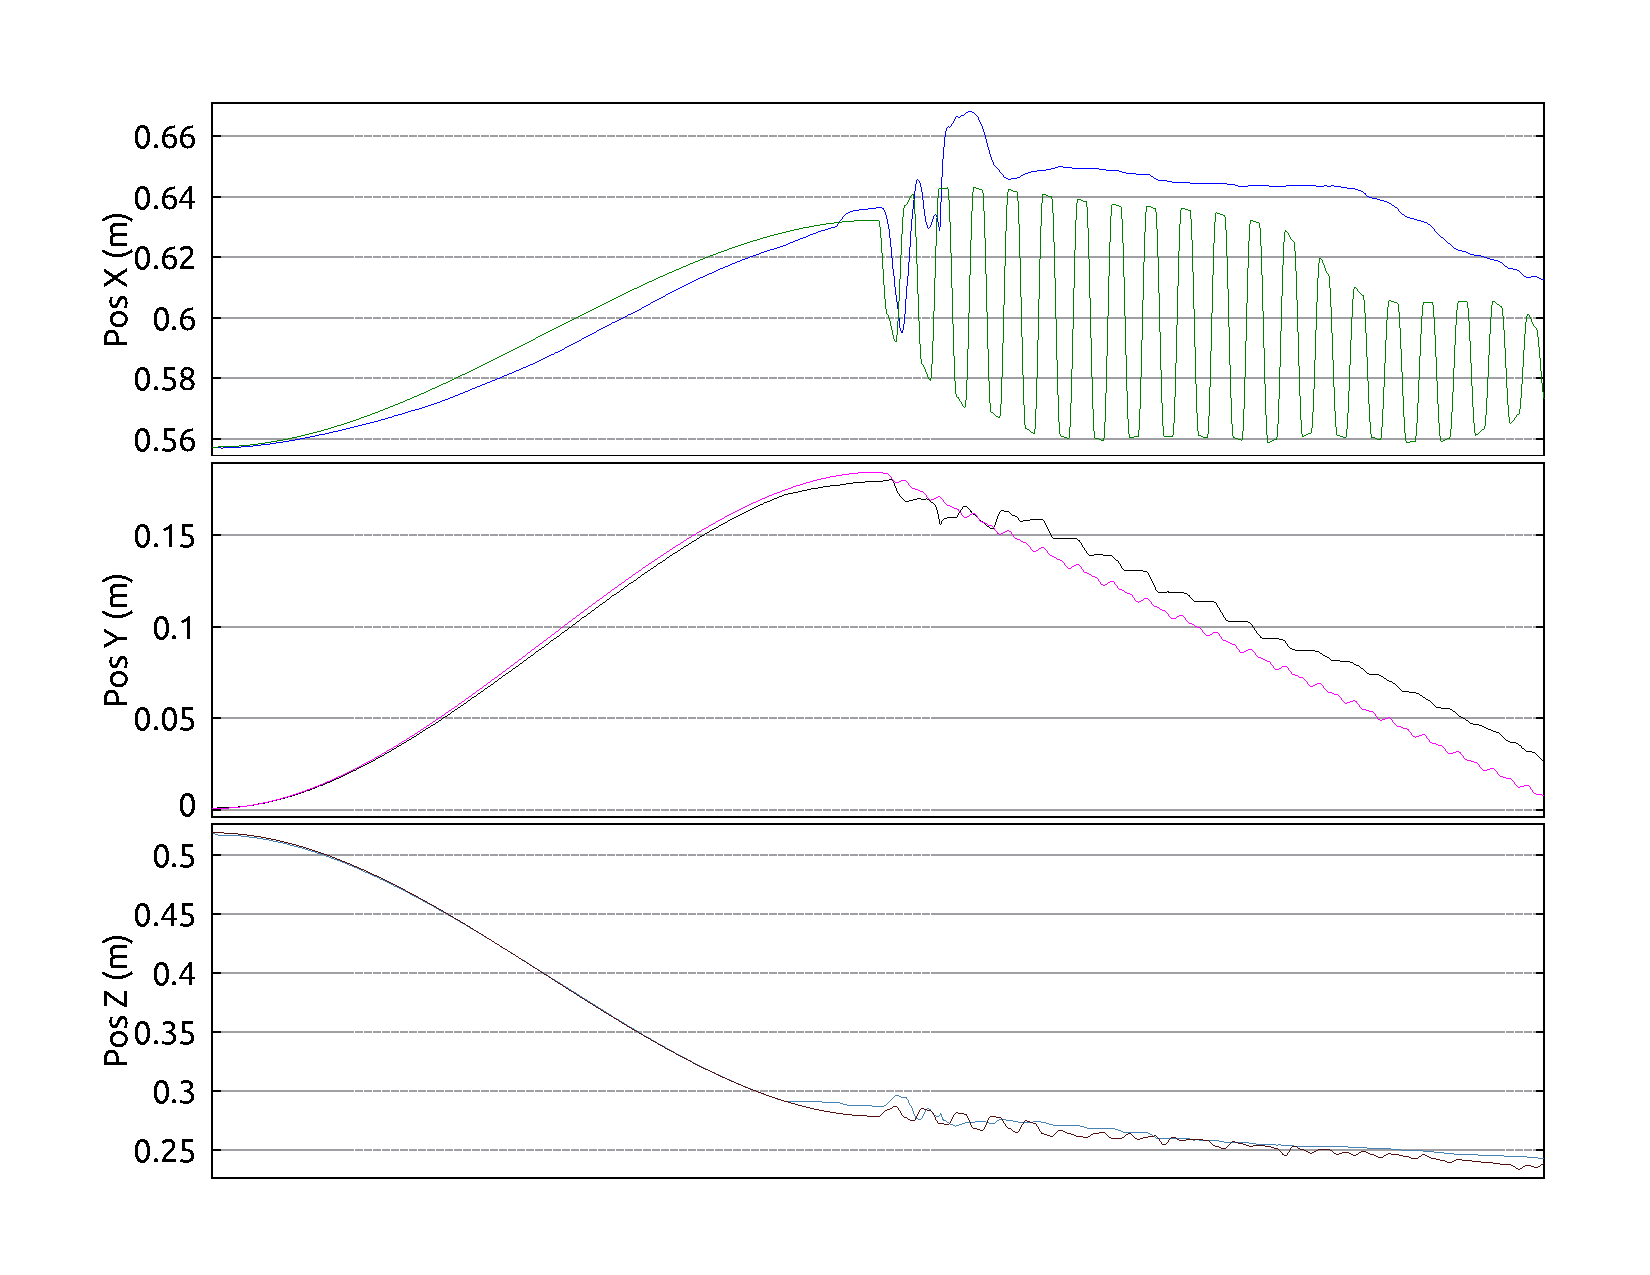
\includegraphics[width=\textwidth]{wound_2_parallel_y_L5_20sec_position_track}
	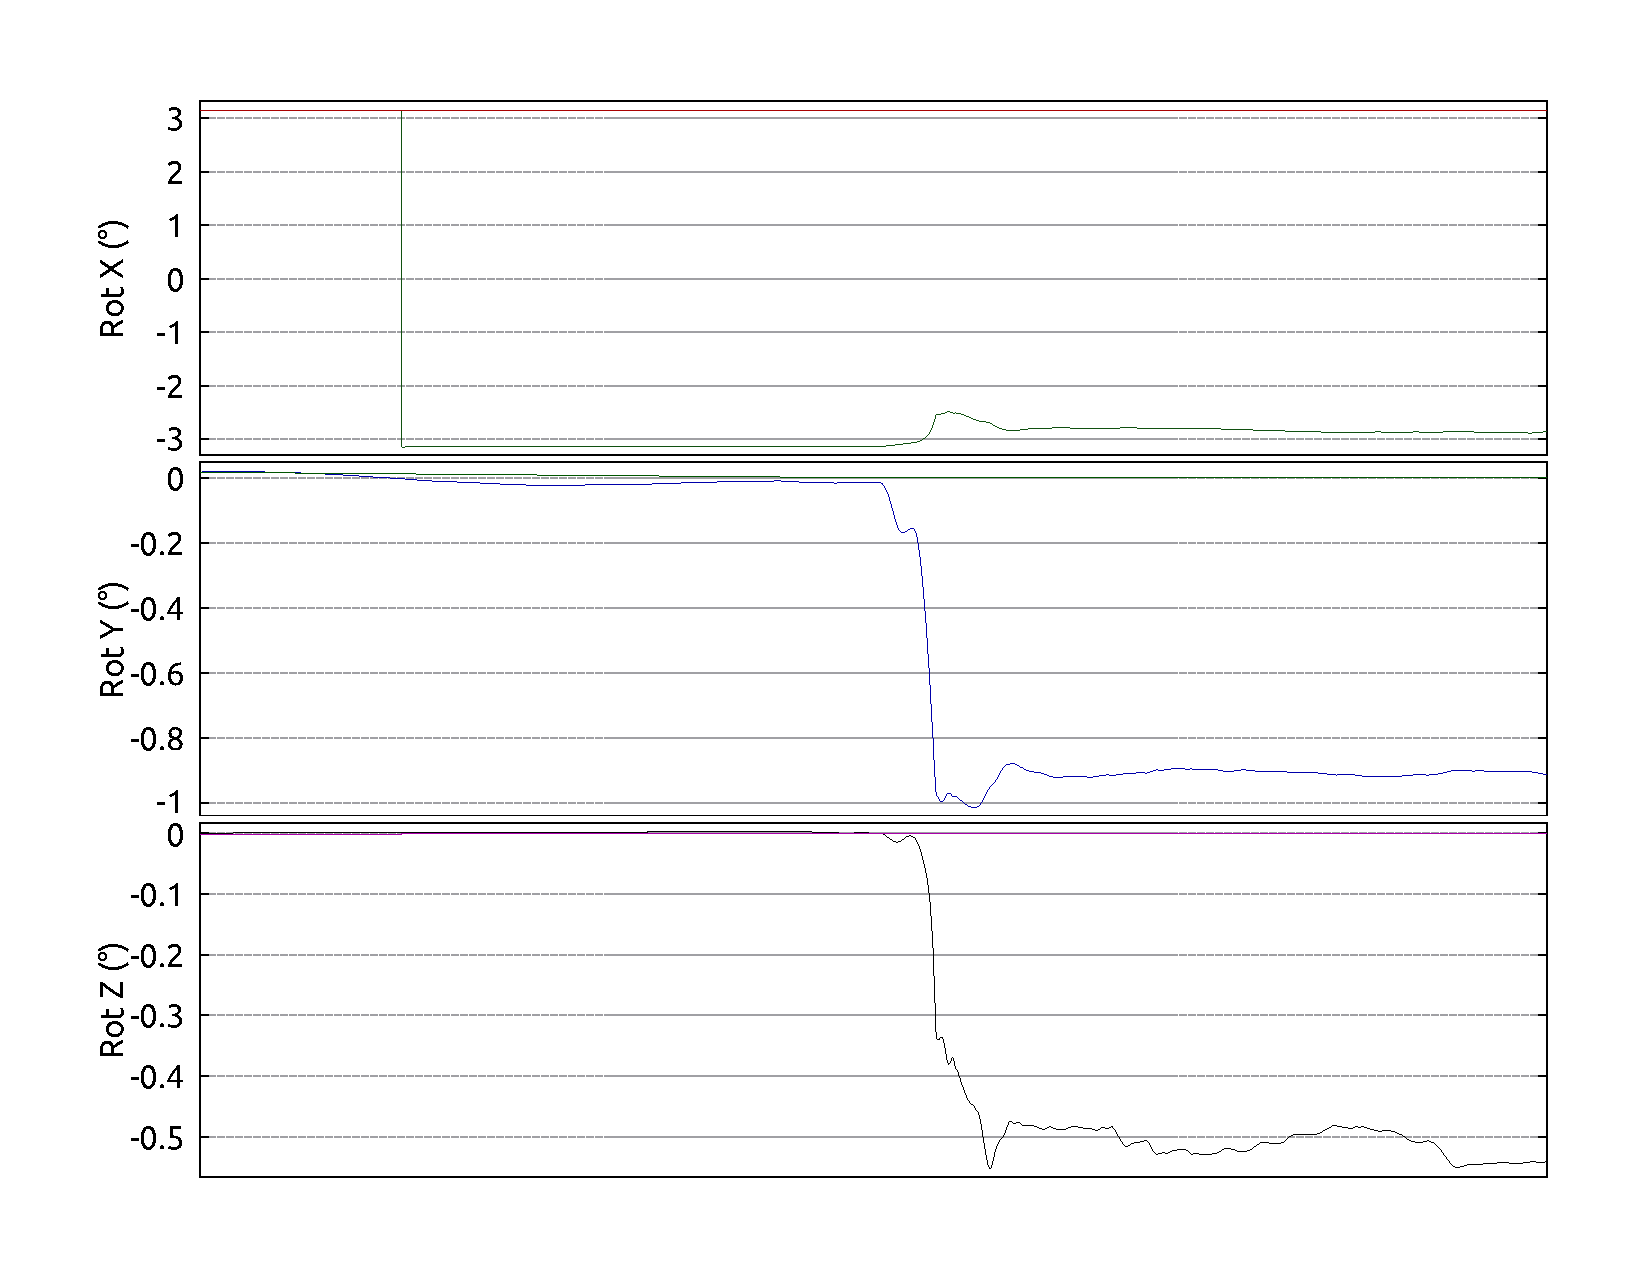
\includegraphics[width=\textwidth]{wound_2_parallel_y_L5_20sec_orientation_track}
    \caption[Wound 3 printing trajectory tracking for Parallel Lines Y path.]{Wound 3 printing trajectory tracking for Parallel Lines Y path. (top) Position tracking. (bottom) Orientation tracking.}
	\label{fig:simulation_test_results_appendix_trajectory_tracking_wound_3_parallel_y_tracking}
\end{figure}

\begin{figure}[htbp]
	\centering
	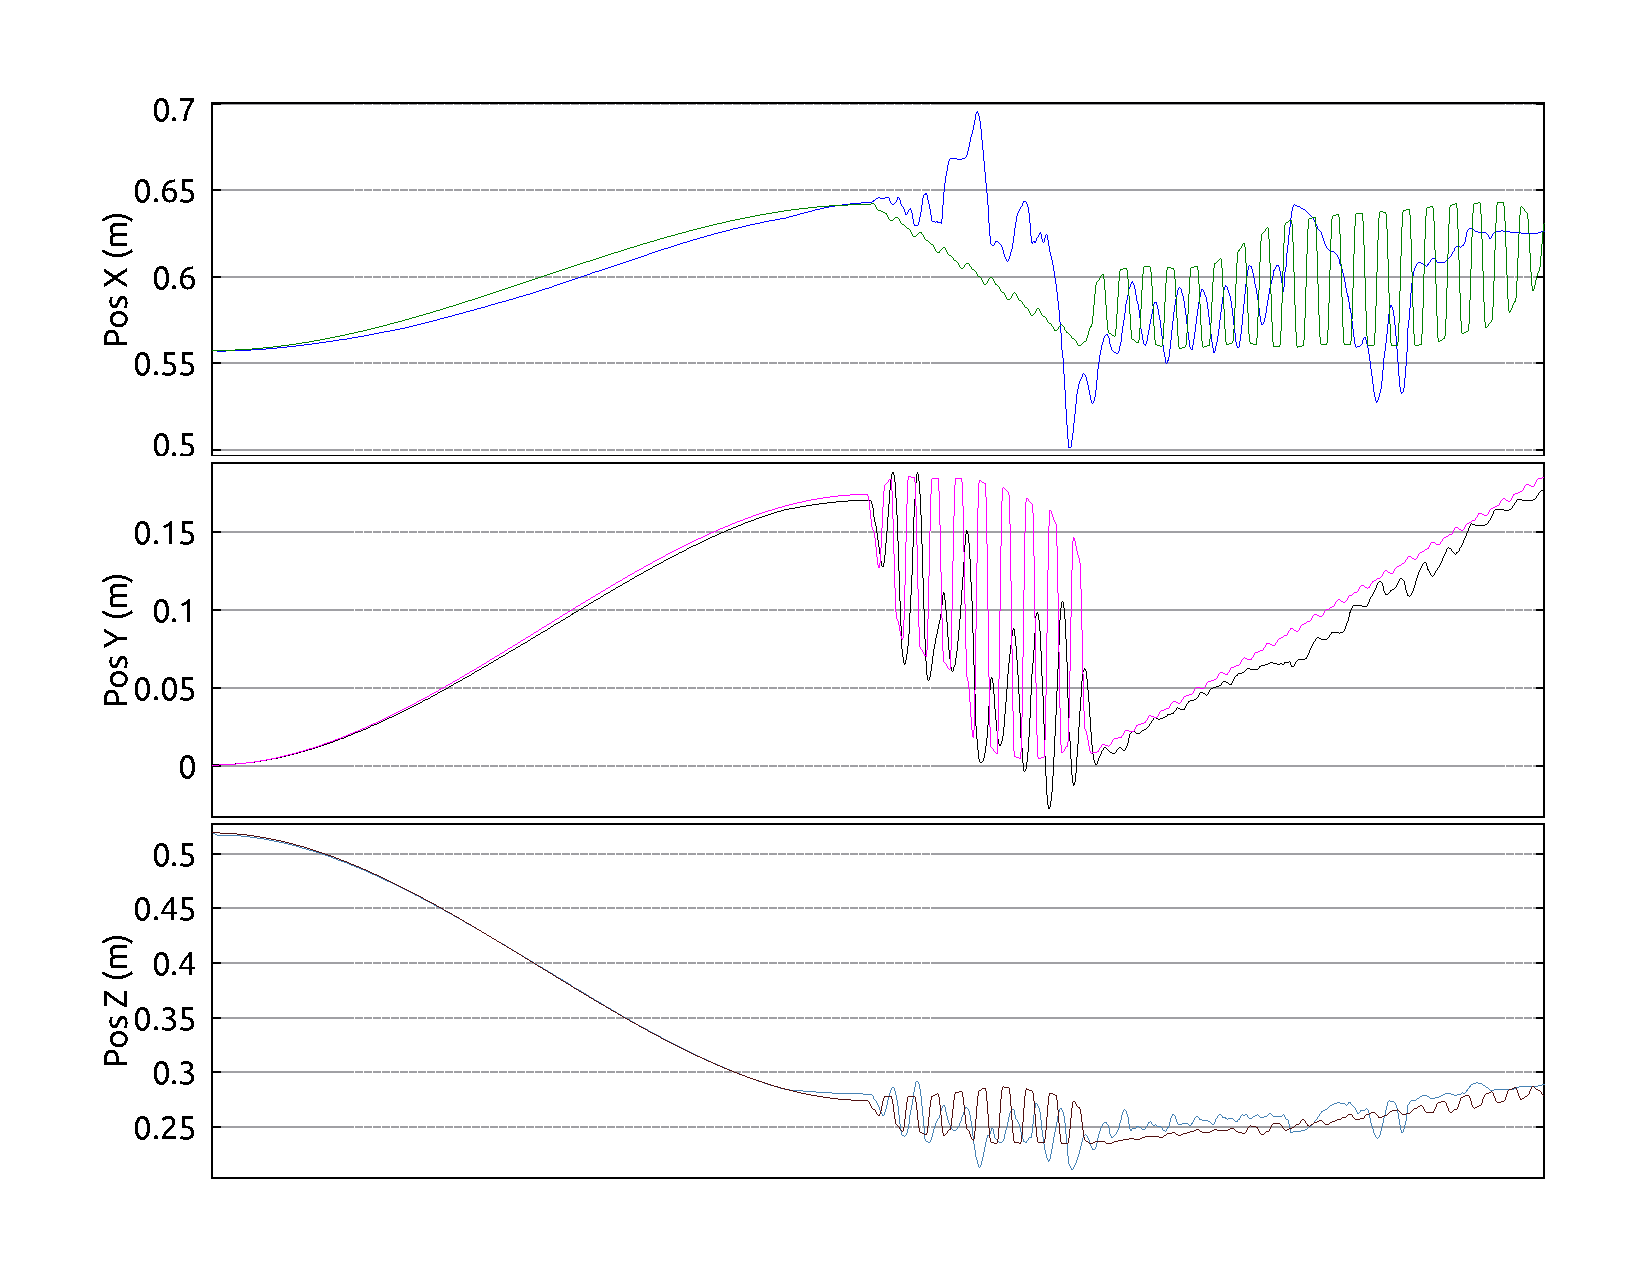
\includegraphics[width=\textwidth]{wound_2_grid_L5_20sec_position_track}
	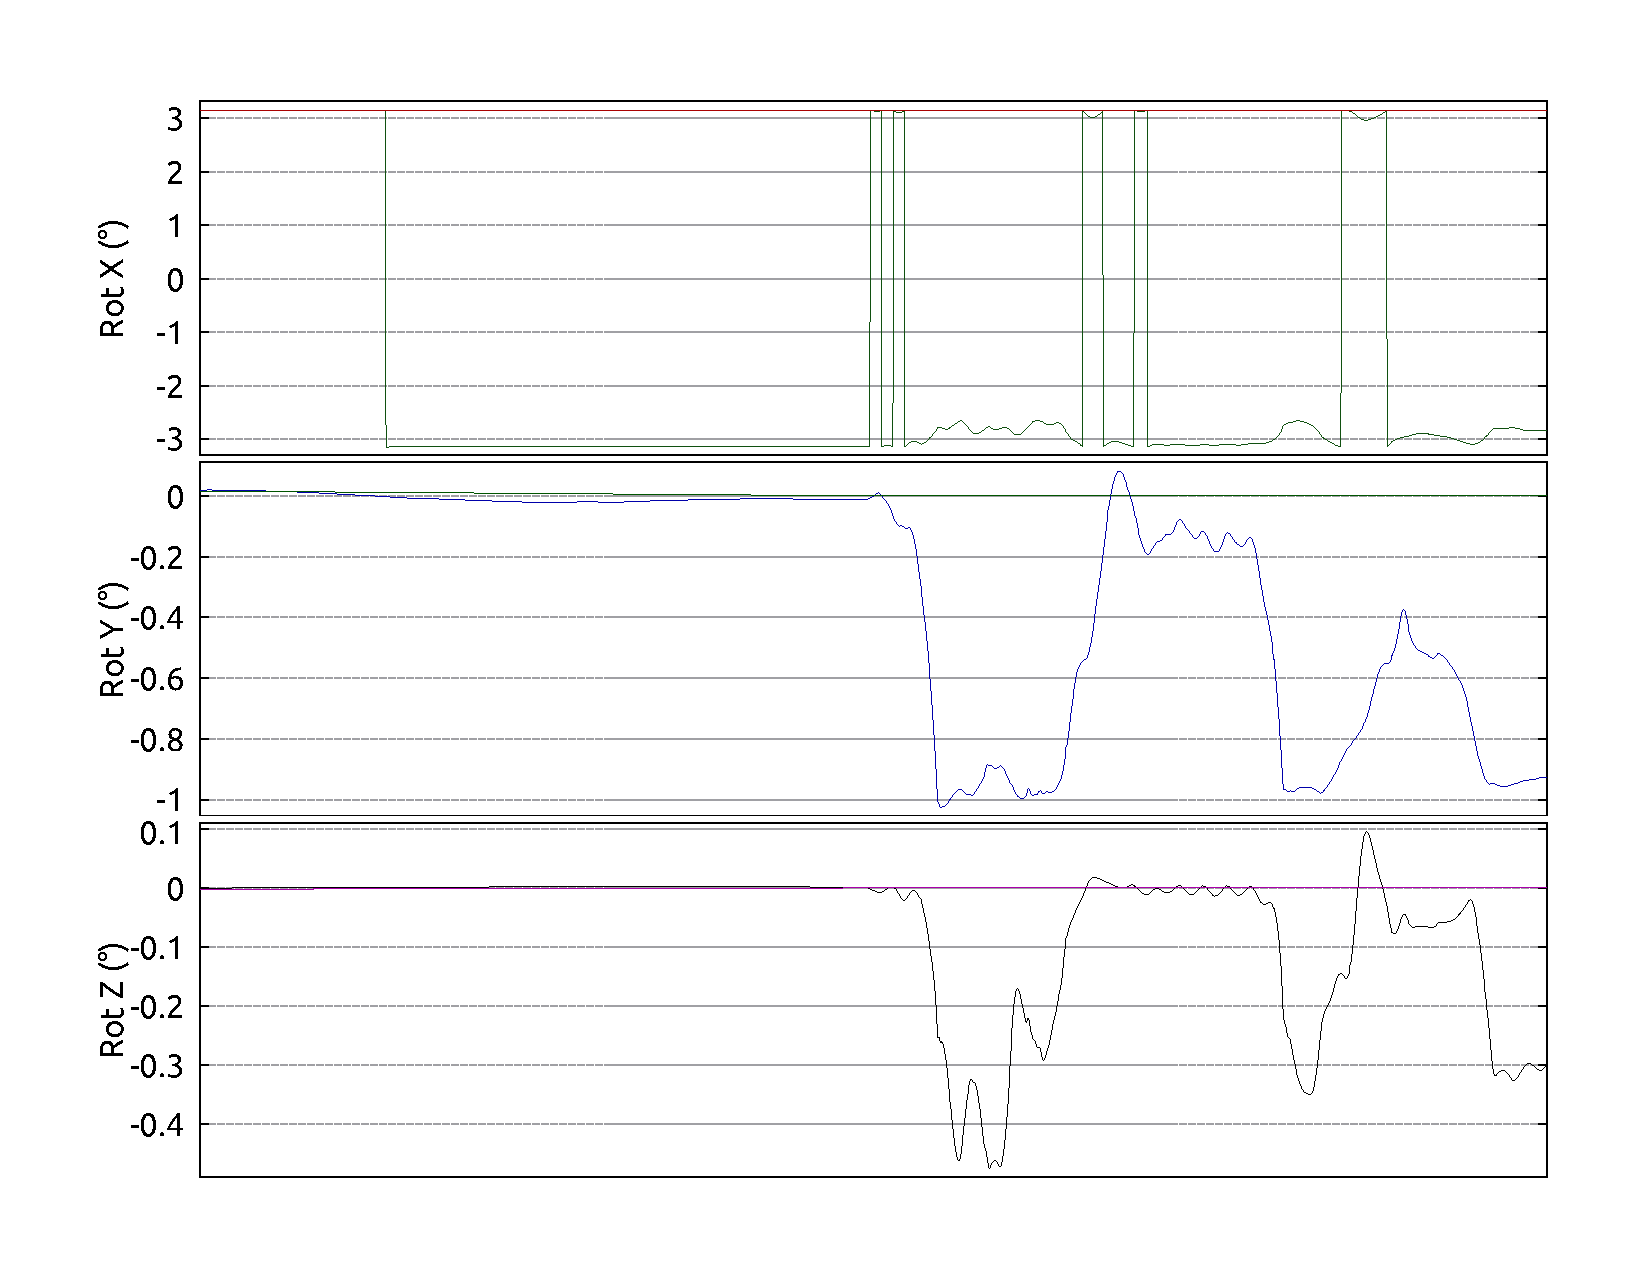
\includegraphics[width=\textwidth]{wound_2_grid_L5_20sec_orientation_track}
    \caption[Wound 3 printing trajectory tracking for Grid path.]{Wound 3 printing trajectory tracking for Grid path. (top) Position tracking. (bottom) Orientation tracking.}
	\label{fig:simulation_test_results_appendix_trajectory_tracking_wound_3_grid_tracking}
\end{figure}

% ------------------------
% Wound 4
% ------------------------

\begin{figure}[htbp]
	\centering
	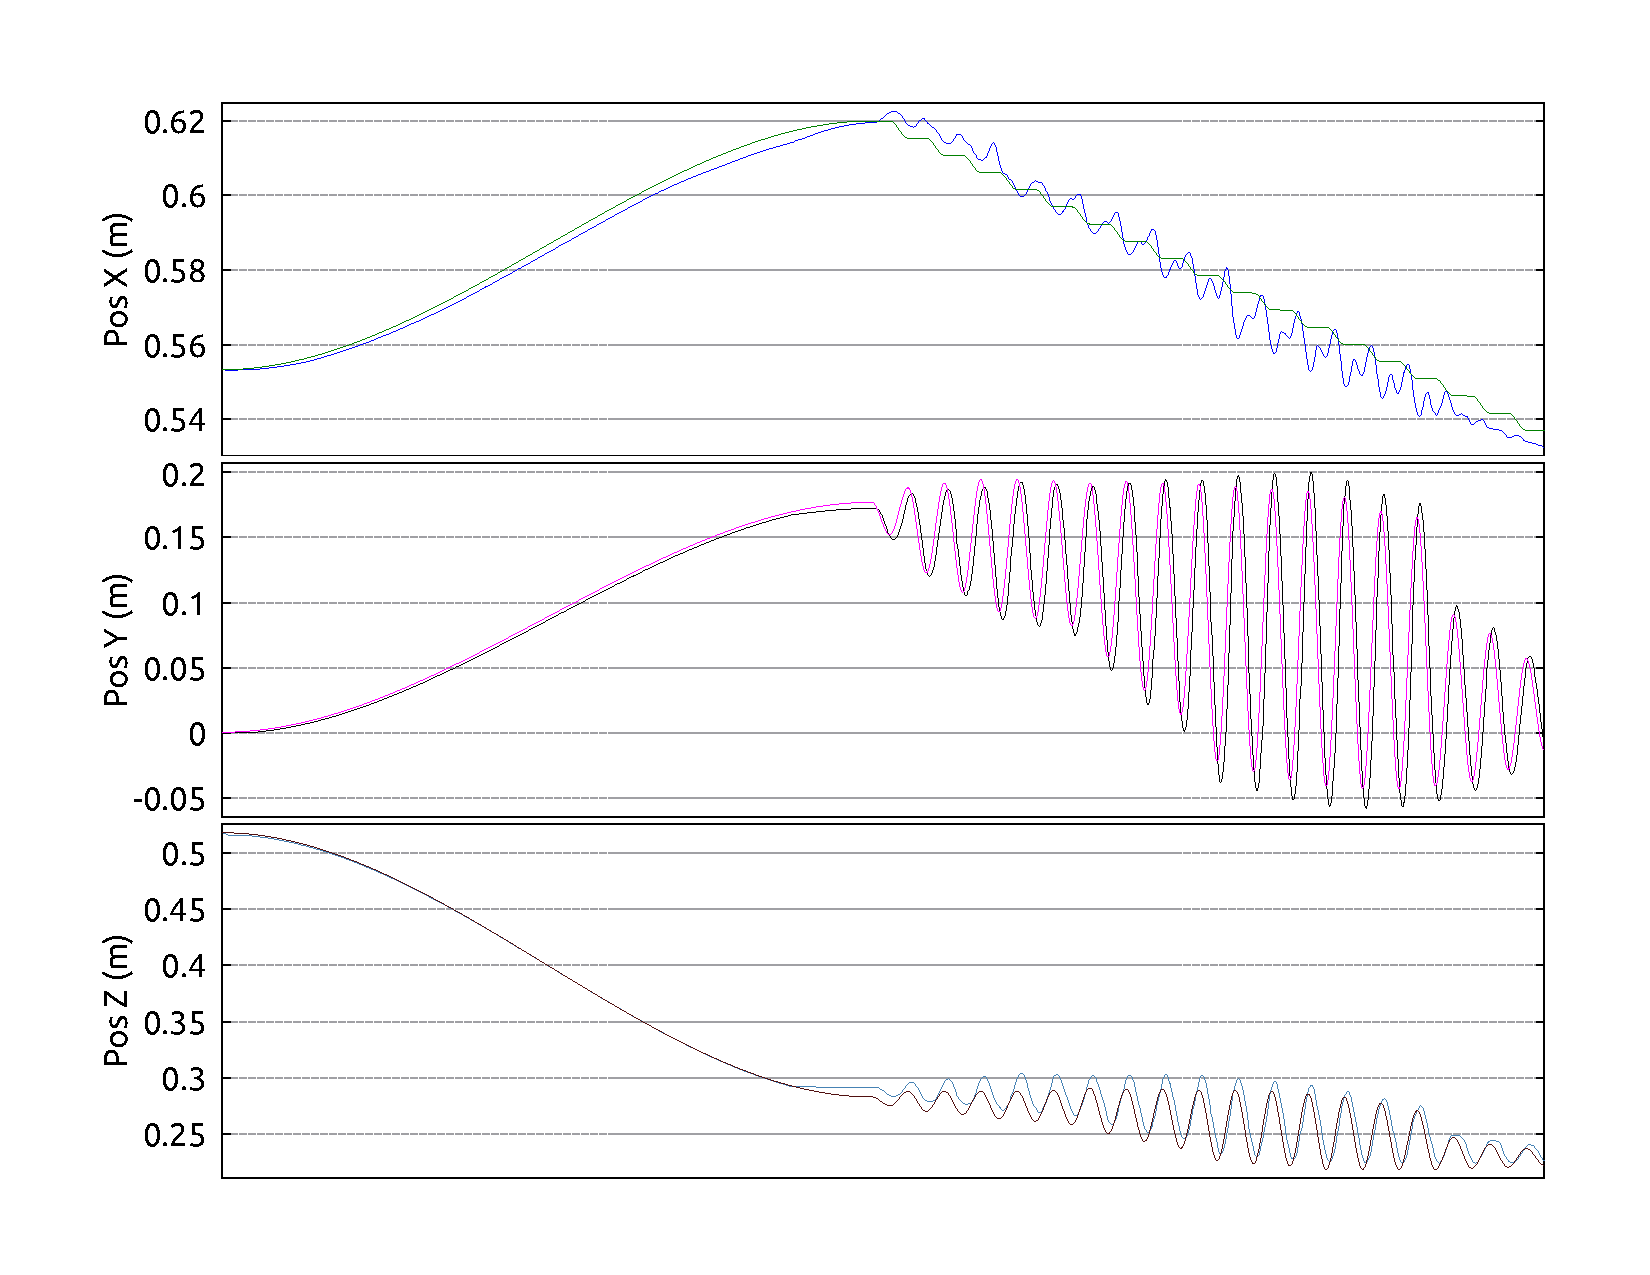
\includegraphics[width=\textwidth]{wound_3_zigzag_x_L5_20sec_position_track}
	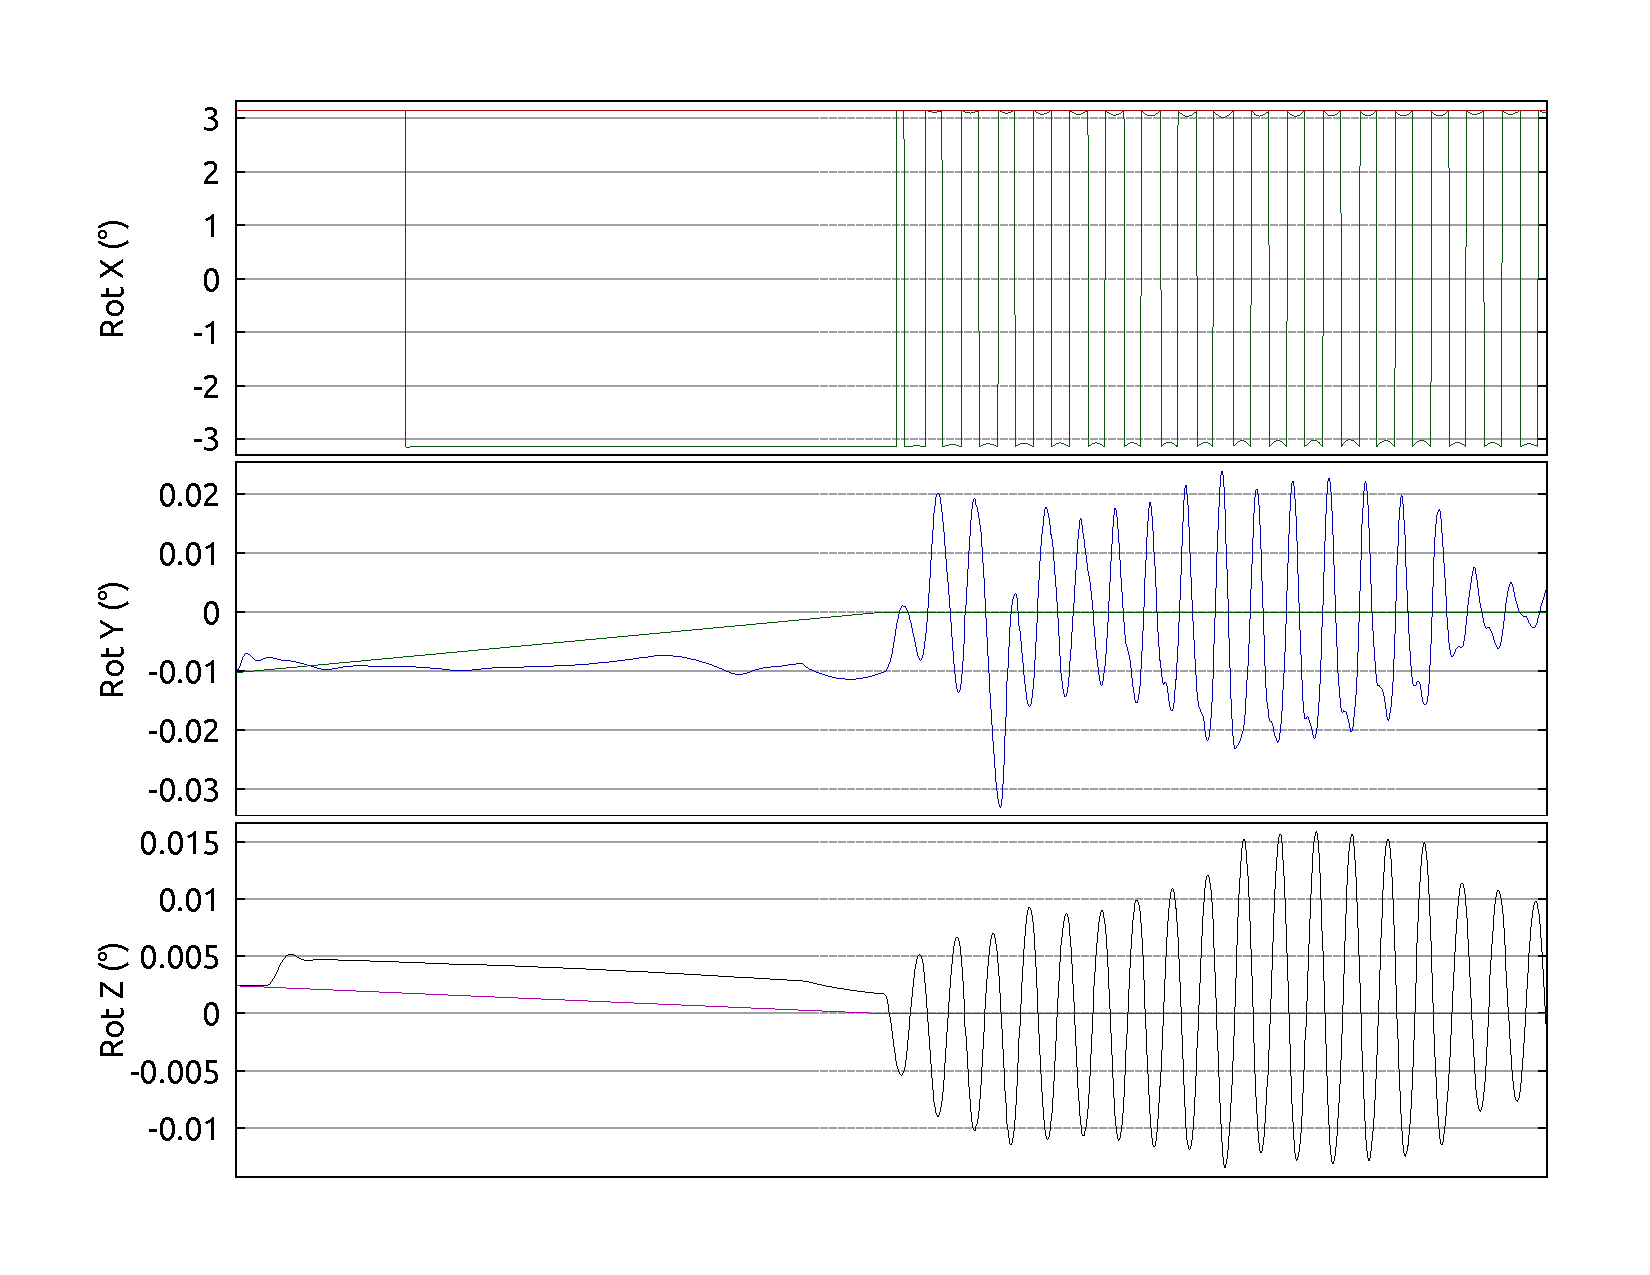
\includegraphics[width=\textwidth]{wound_3_zigzag_x_L5_20sec_orientation_track}
	\caption[Wound 4 printing trajectory tracking for ZigZag X path.]{Wound 4 printing trajectory tracking for ZigZag X path. (top) Position tracking. (bottom) Orientation tracking.}
    \label{fig:simulation_test_results_appendix_trajectory_tracking_wound_4_zizzag_x_tracking}
\end{figure}

\begin{figure}[htbp]
	\centering
	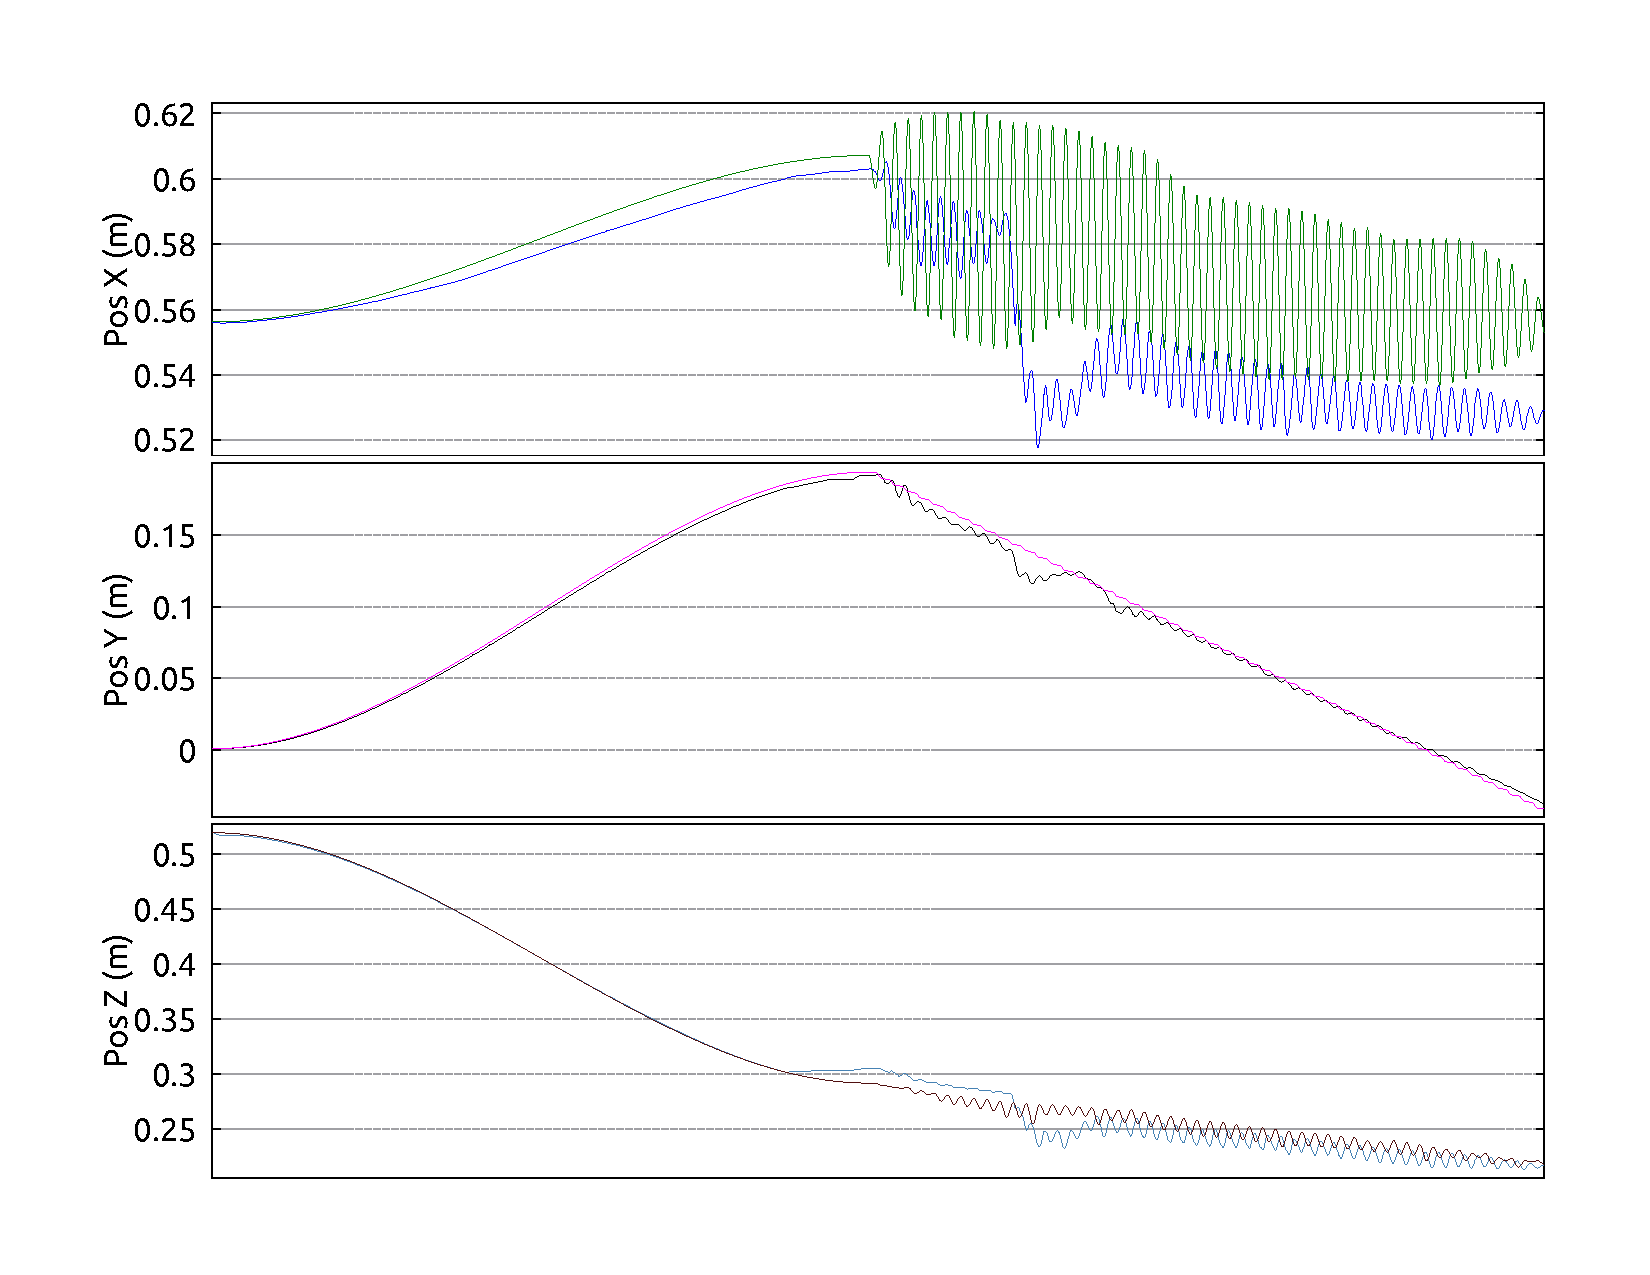
\includegraphics[width=\textwidth]{wound_3_zigzag_y_L5_20sec_position_track}
	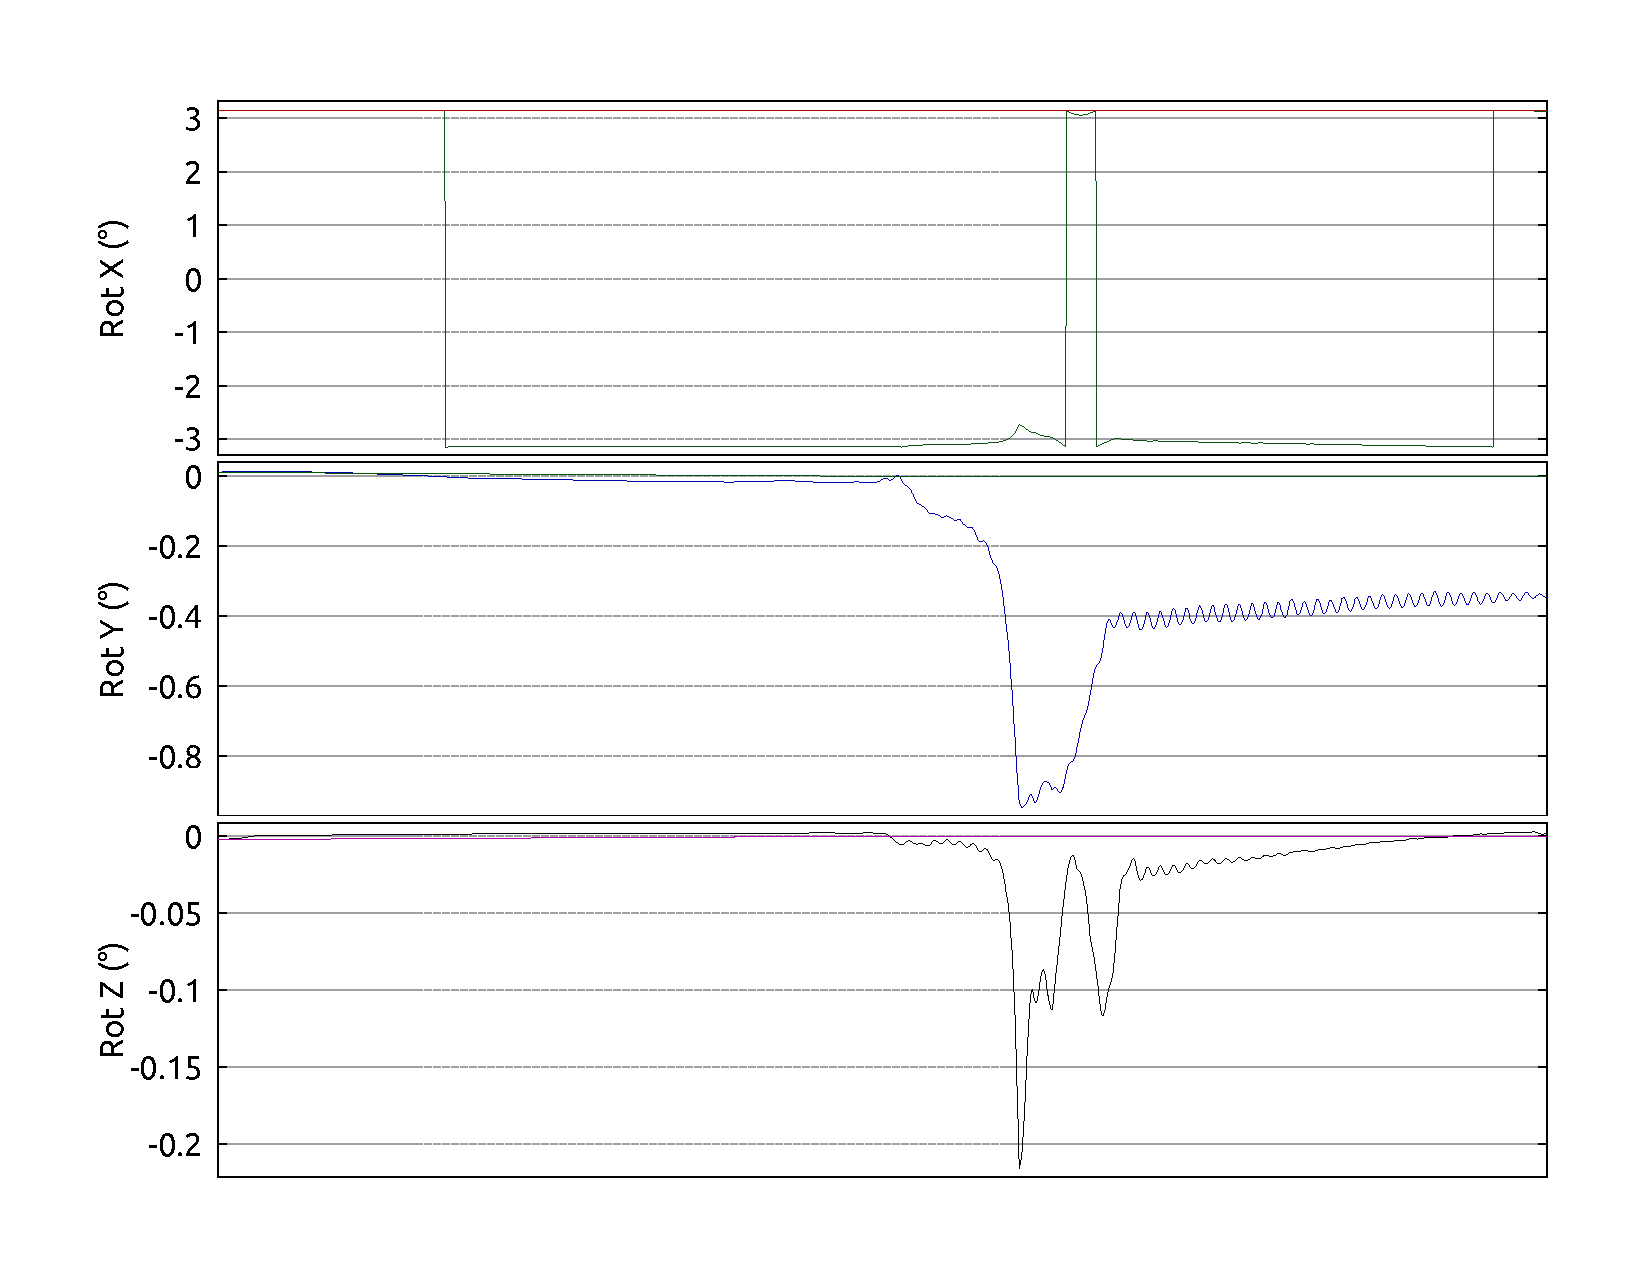
\includegraphics[width=\textwidth]{wound_3_zigzag_y_L5_20sec_orientation_track}
\caption[Wound 4 printing trajectory tracking for ZigZag Y path.]{Wound 4 printing trajectory tracking for ZigZag Y path. (top) Position tracking. (bottom) Orientation tracking.}
	\label{fig:simulation_test_results_appendix_trajectory_tracking_wound_4_zizzag_y_tracking}
\end{figure}

\begin{figure}[htbp]
	\centering
	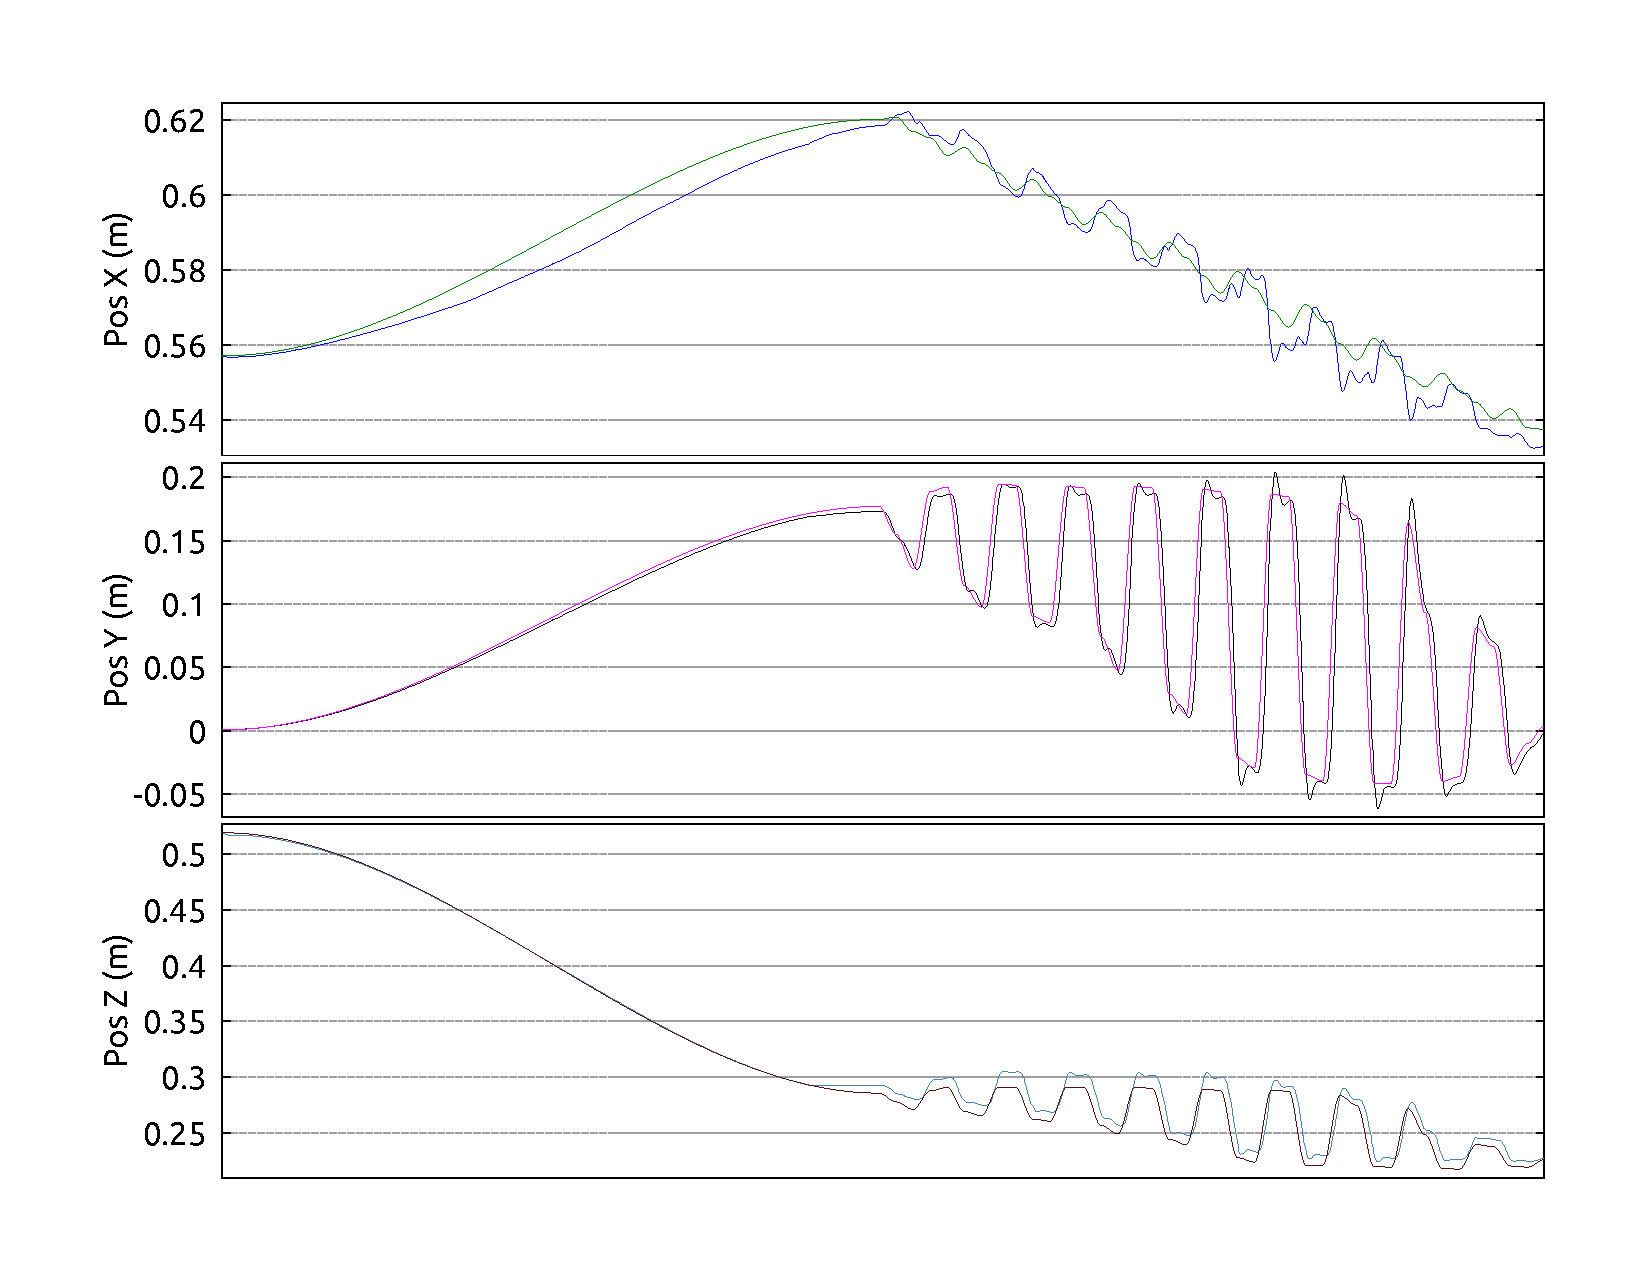
\includegraphics[width=\textwidth]{wound_3_parallel_x_L5_20sec_position_track}
	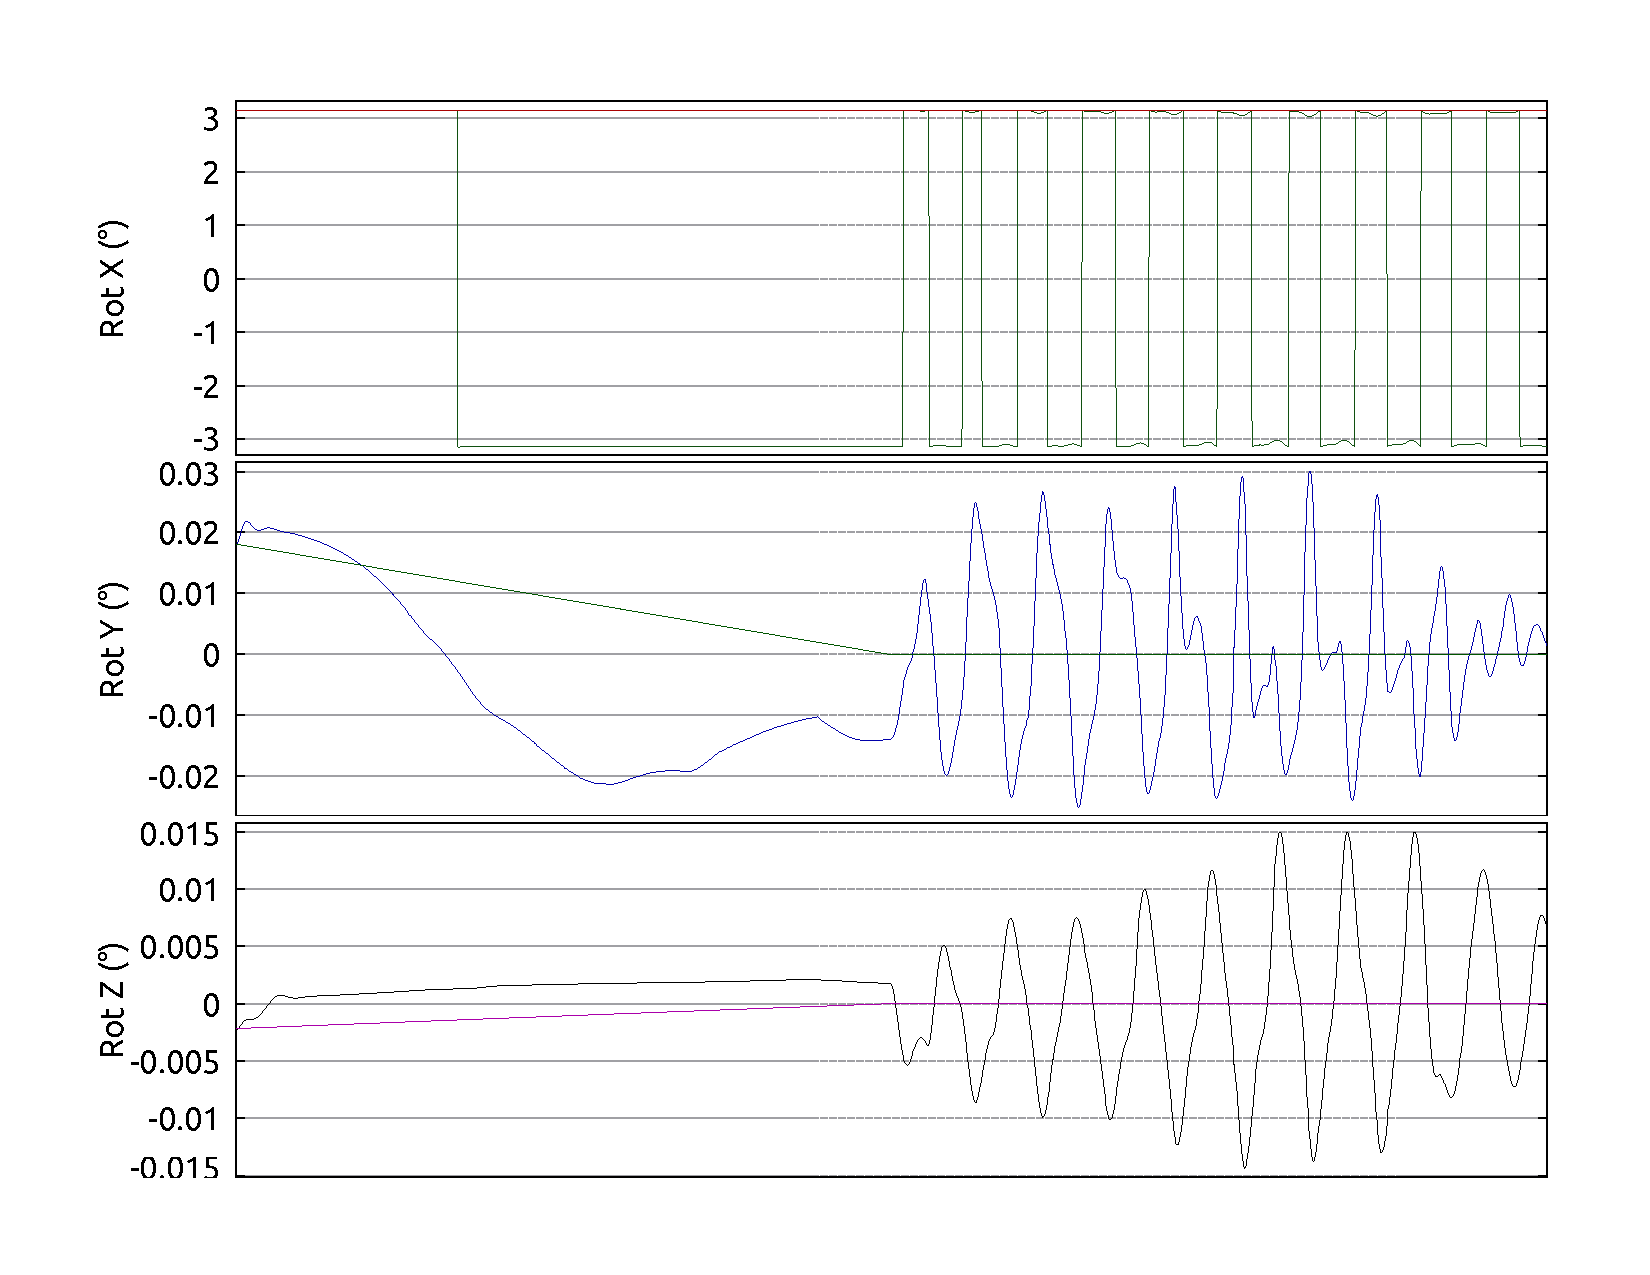
\includegraphics[width=\textwidth]{wound_3_parallel_x_L5_20sec_orientation_track}
	\caption[Wound 4 printing trajectory tracking for Parallel Lines X path.]{Wound 4 printing trajectory tracking for Parallel Lines X path. (top) Position tracking. (bottom) Orientation tracking.}
	\label{fig:simulation_test_results_appendix_trajectory_tracking_wound_4_parallel_x_tracking}
\end{figure}

\begin{figure}[htbp]
	\centering
	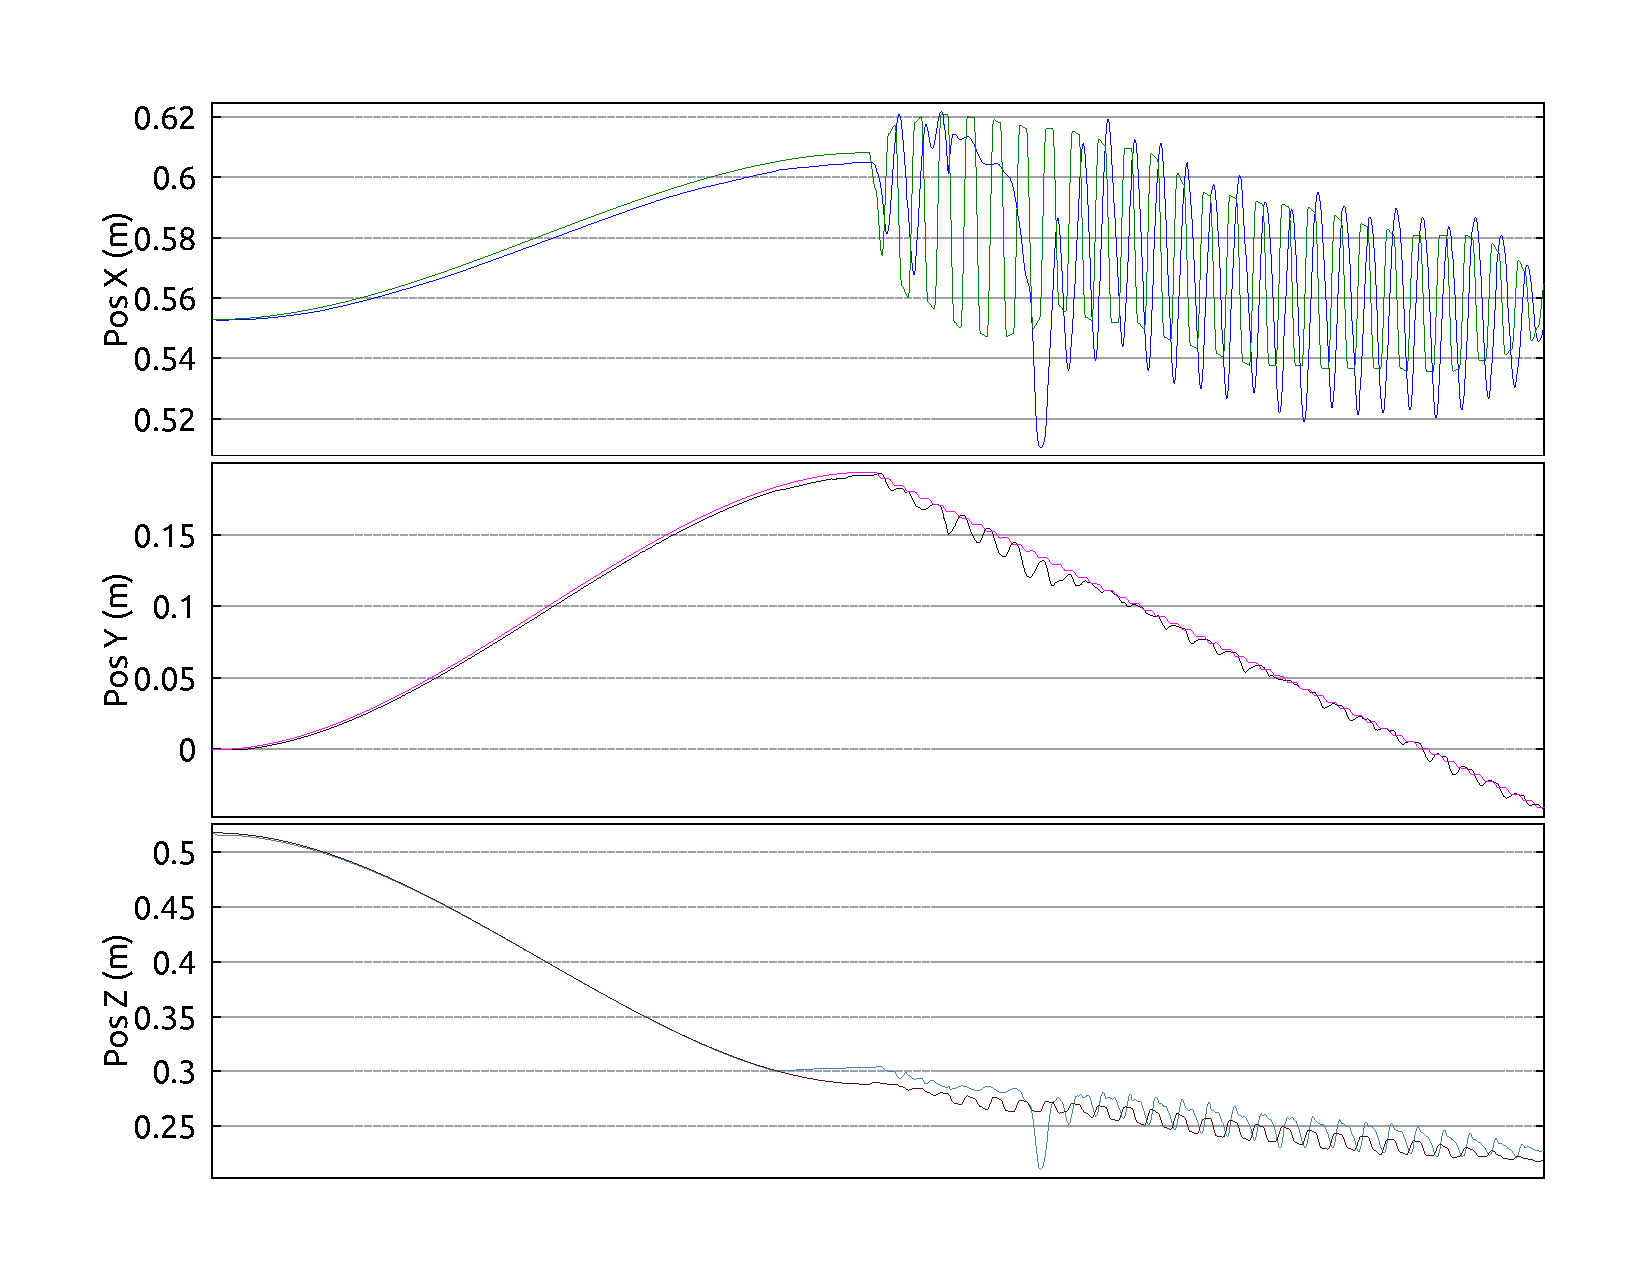
\includegraphics[width=\textwidth]{wound_3_parallel_y_L5_20sec_position_track}
	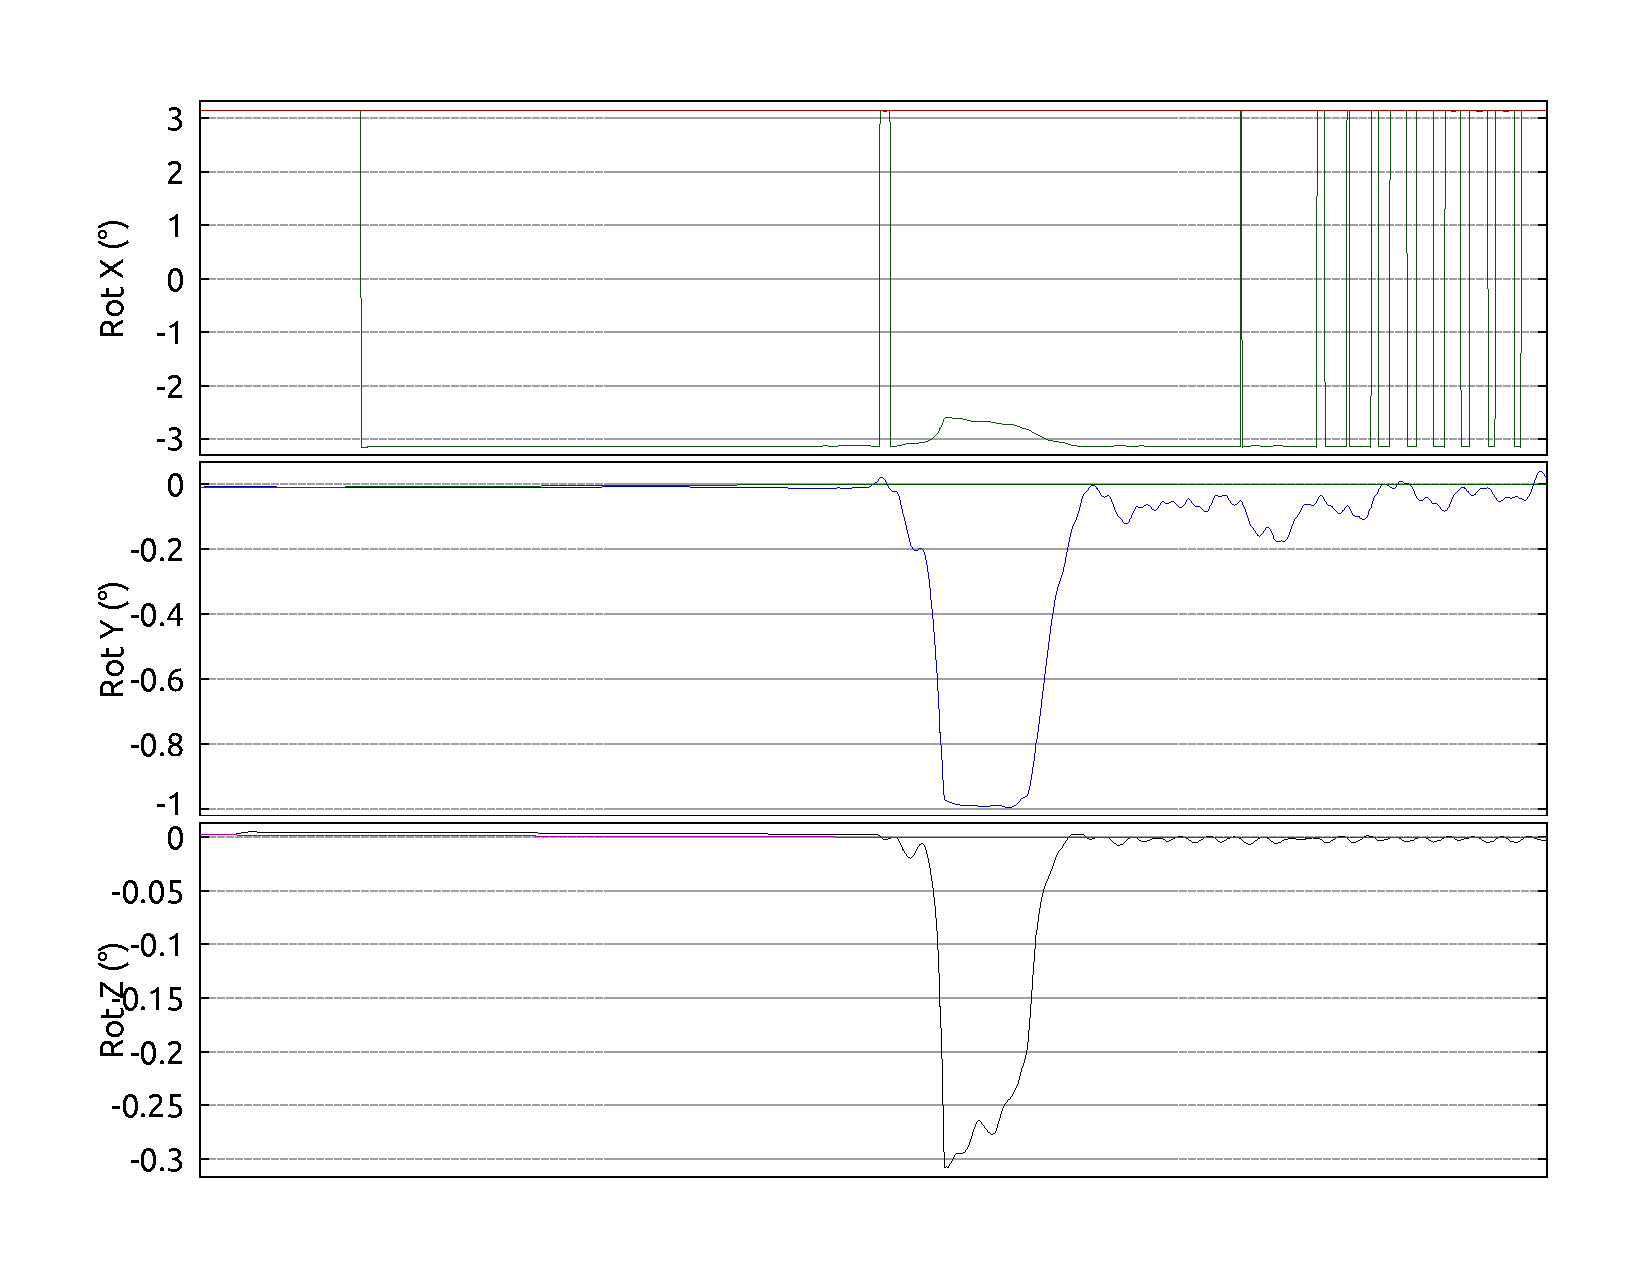
\includegraphics[width=\textwidth]{wound_3_parallel_y_L5_20sec_orientation_track}
    \caption[Wound 4 printing trajectory tracking for Parallel Lines Y path.]{Wound 4 printing trajectory tracking for Parallel Lines Y path. (top) Position tracking. (bottom) Orientation tracking.}
	\label{fig:simulation_test_results_appendix_trajectory_tracking_wound_4_parallel_y_tracking}
\end{figure}

\begin{figure}[htbp]
	\centering
	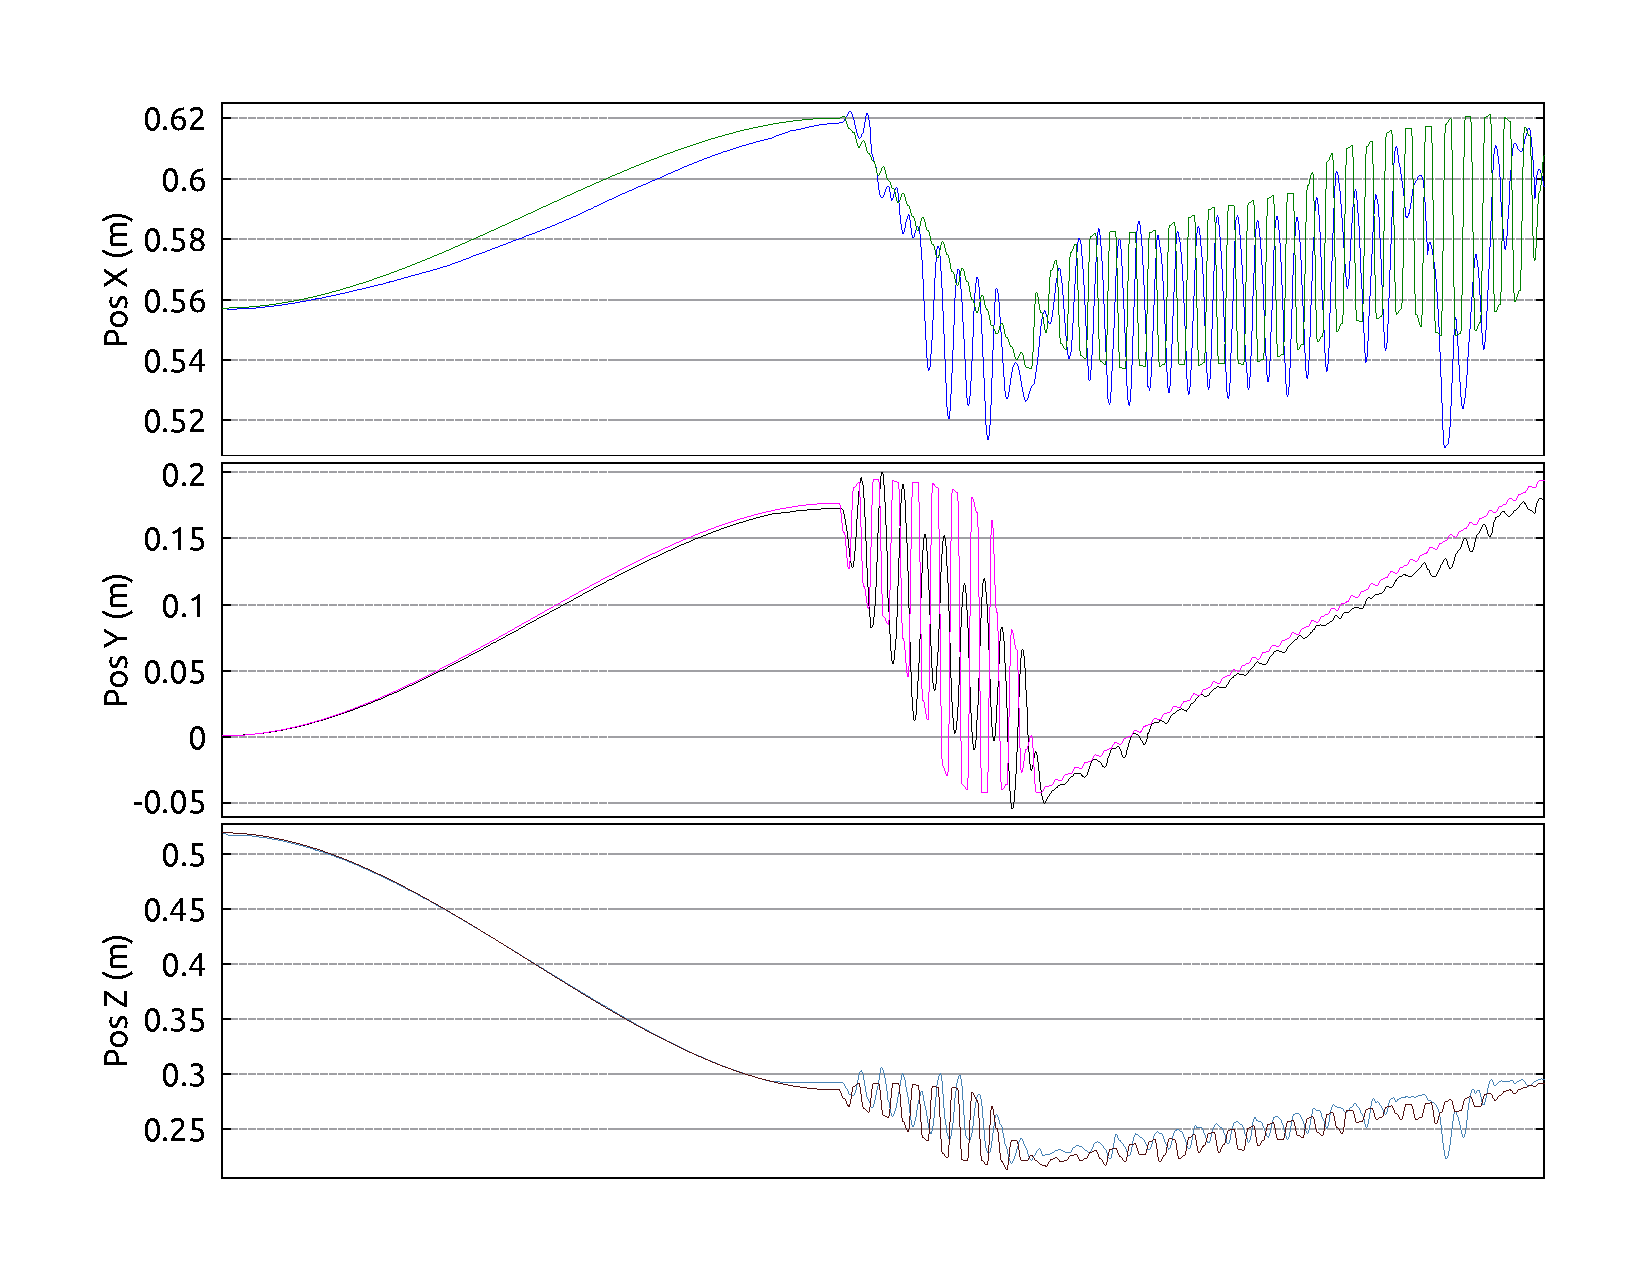
\includegraphics[width=\textwidth]{wound_3_grid_L5_20sec_position_track}
	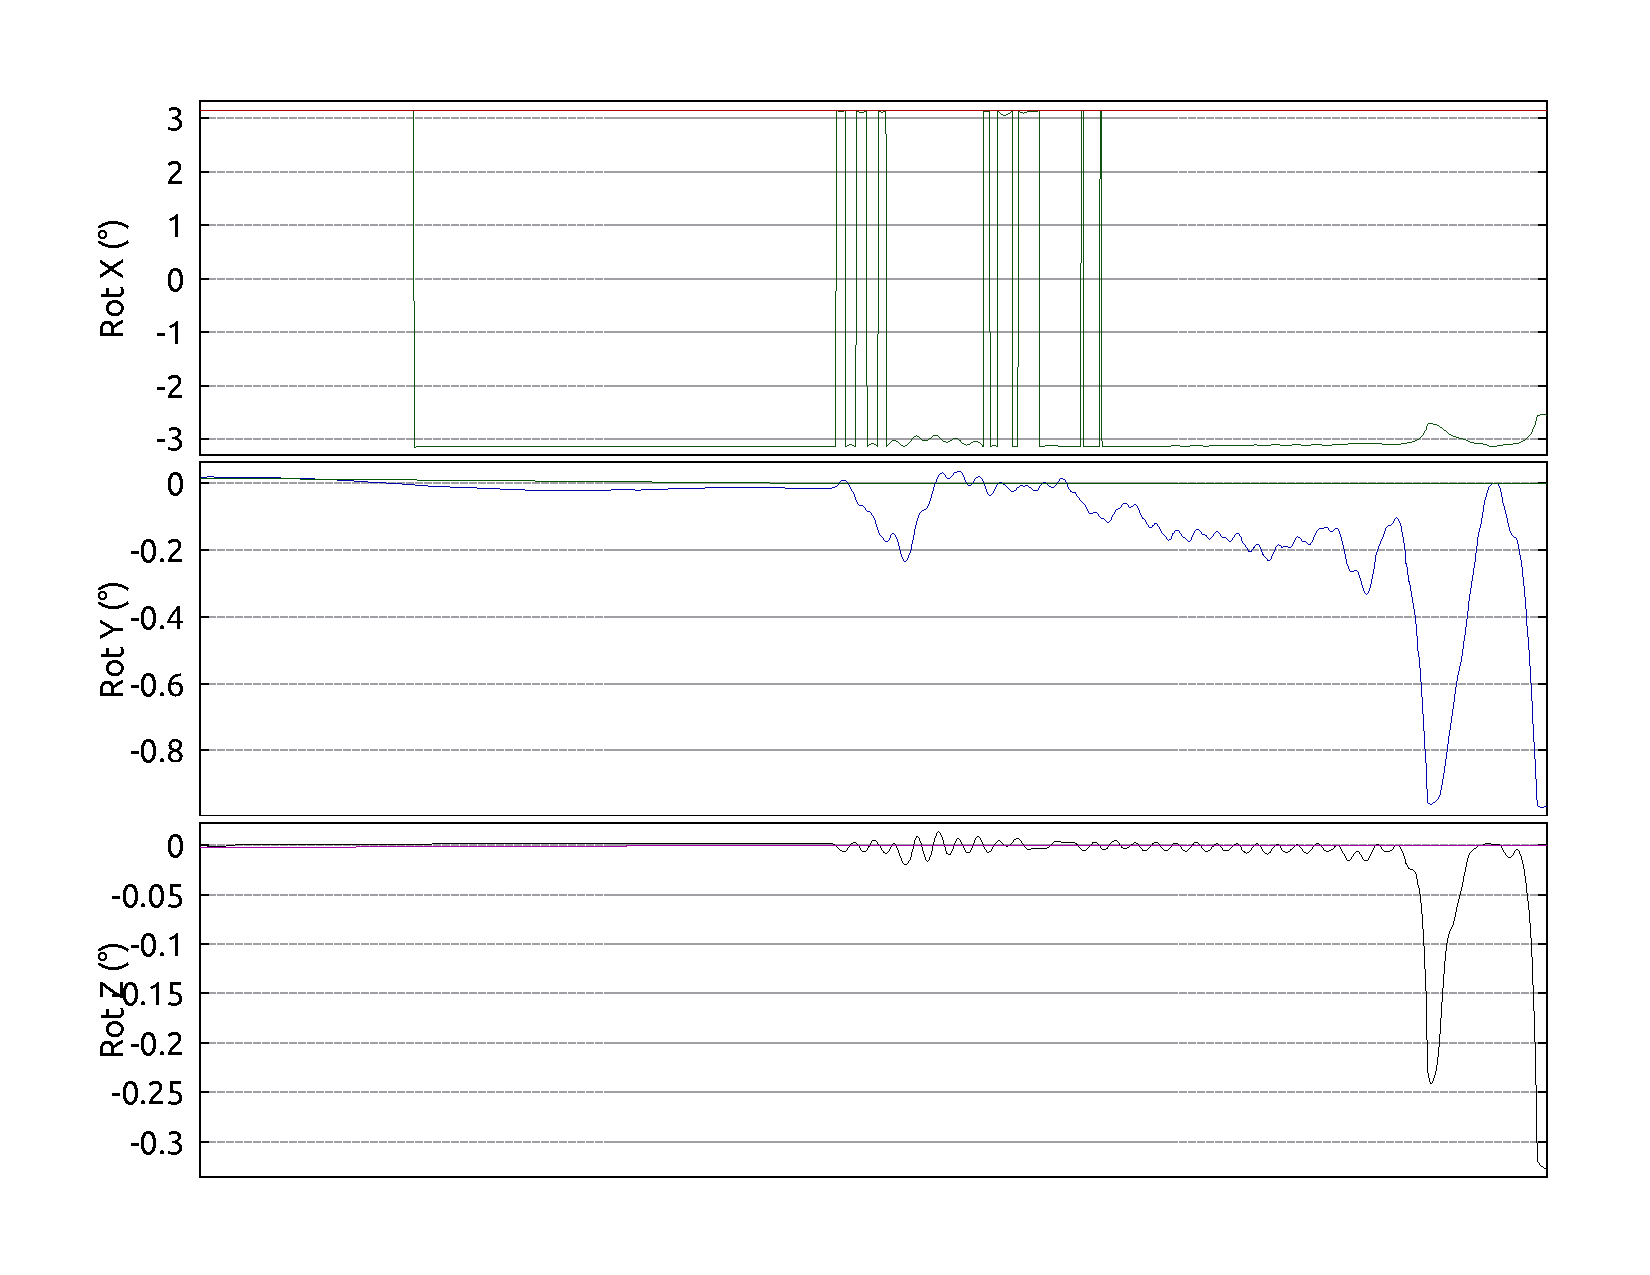
\includegraphics[width=\textwidth]{wound_3_grid_L5_20sec_orientation_track}
    \caption[Wound 4 printing trajectory tracking for Grid path.]{Wound 4 printing trajectory tracking for Grid path. (top) Position tracking. (bottom) Orientation tracking.}
	\label{fig:simulation_test_results_appendix_trajectory_tracking_wound_4_grid_tracking}
\end{figure}

% ------------------------
% Wound 5
% ------------------------

\begin{figure}[htbp]
	\centering
	\includegraphics[width=\textwidth]{wound_4_zigzag_x_L5_20sec_position_track}
	\includegraphics[width=\textwidth]{wound_4_zigzag_x_L5_20sec_orientation_track}
	\caption[Wound 5 printing trajectory tracking for ZigZag X path.]{Wound 5 printing trajectory tracking for ZigZag X path. (top) Position tracking. (bottom) Orientation tracking.}
    \label{fig:simulation_test_results_appendix_trajectory_tracking_wound_5_zizzag_x_tracking}
\end{figure}


\begin{figure}[htbp]
	\centering
	\includegraphics[width=\textwidth]{wound_4_zigzag_y_L5_20sec_position_track}
	\includegraphics[width=\textwidth]{wound_4_zigzag_y_L5_20sec_orientation_track}
\caption[Wound 5 printing trajectory tracking for ZigZag Y path.]{Wound 5 printing trajectory tracking for ZigZag Y path. (top) Position tracking. (bottom) Orientation tracking.}
	\label{fig:simulation_test_results_appendix_trajectory_tracking_wound_5_zizzag_y_tracking}
\end{figure}


\begin{figure}[htbp]
	\centering
	\includegraphics[width=\textwidth]{wound_4_parallel_x_L5_20sec_position_track}
	\includegraphics[width=\textwidth]{wound_4_parallel_x_L5_20sec_orientation_track}
	\caption[Wound 5 printing trajectory tracking for Parallel Lines X path.]{Wound 5 printing trajectory tracking for Parallel Lines X path. (top) Position tracking. (bottom) Orientation tracking.}
	\label{fig:simulation_test_results_appendix_trajectory_tracking_wound_5_parallel_x_tracking}
\end{figure}

\begin{figure}[htbp]
	\centering
	\includegraphics[width=\textwidth]{wound_4_parallel_y_L5_20sec_position_track}
	\includegraphics[width=\textwidth]{wound_4_parallel_y_L5_20sec_orientation_track}
    \caption[Wound 5 printing trajectory tracking for Parallel Lines Y path.]{Wound 5 printing trajectory tracking for Parallel Lines Y path. (top) Position tracking. (bottom) Orientation tracking.}
	\label{fig:simulation_test_results_appendix_trajectory_tracking_wound_5_parallel_y_tracking}
\end{figure}

\begin{figure}[htbp]
	\centering
	\includegraphics[width=\textwidth]{wound_4_grid_L5_20sec_position_track}
	\includegraphics[width=\textwidth]{wound_4_grid_L5_20sec_orientation_track}
    \caption[Wound 5 printing trajectory tracking for Grid path.]{Wound 5 printing trajectory tracking for Grid path. (top) Position tracking. (bottom) Orientation tracking.}
	\label{fig:simulation_test_results_appendix_trajectory_tracking_wound_5_grid_tracking}
\end{figure}

% section simulation_test_results_appendix_bioprinting_directly_wound